\par In this chapter, the new COSY routines are benchmarked against both ICOOL and G4Beamline for pencil beams. Recall that a pencil beam is a beam with an RMS of zero for all transverse coordinates. Pencil beams are used in order to simulate a plethora of possible paths and energy losses for a particular initial condition. Both validation against past experiments and predictions of current muon ionization cooling channel efforts are also shown. Since both ICOOL and G4Beamline have automatic variable stepping, their step sizes are left as default unless explicitly stated otherwise.

\Section{Benchmark Against Other Codes}\label{sec:benchmark}

This section briefly discusses the comparison of the new COSY routines with those of two other codes, ICOOL \cite{icool} and G4Beamline \cite{g4bl}. Refer to Figures \ref{fig:100.1}--\ref{fig:400.100} (12 figures, each with three subplots) mentioned here. The benchmarking was done over both the typical momentum range of cooling channels (100, 200, 300, and 400 MeV/$c$) and various absorber lengths (1, 10, and 100 mm). These simulations were performed using a pencil beam of $5\times 10^4$ muons with the aforementioned momenta through liquid hydrogen. Note that for the transverse position and transverse momentum histograms, the absolute value of the coordinate is plotted. Therefore, the mean is not zero. For COSY, the step size was the entire absorber length. For G4Beamline in the case of a 1 mm absorber, the maximum step size was limited to 0.1 mm. This was done because of the heavy dependence of the transverse position on step size for short absorbers in G4Beamline.
\newpage
\begin{figure}[H]
  \centering
    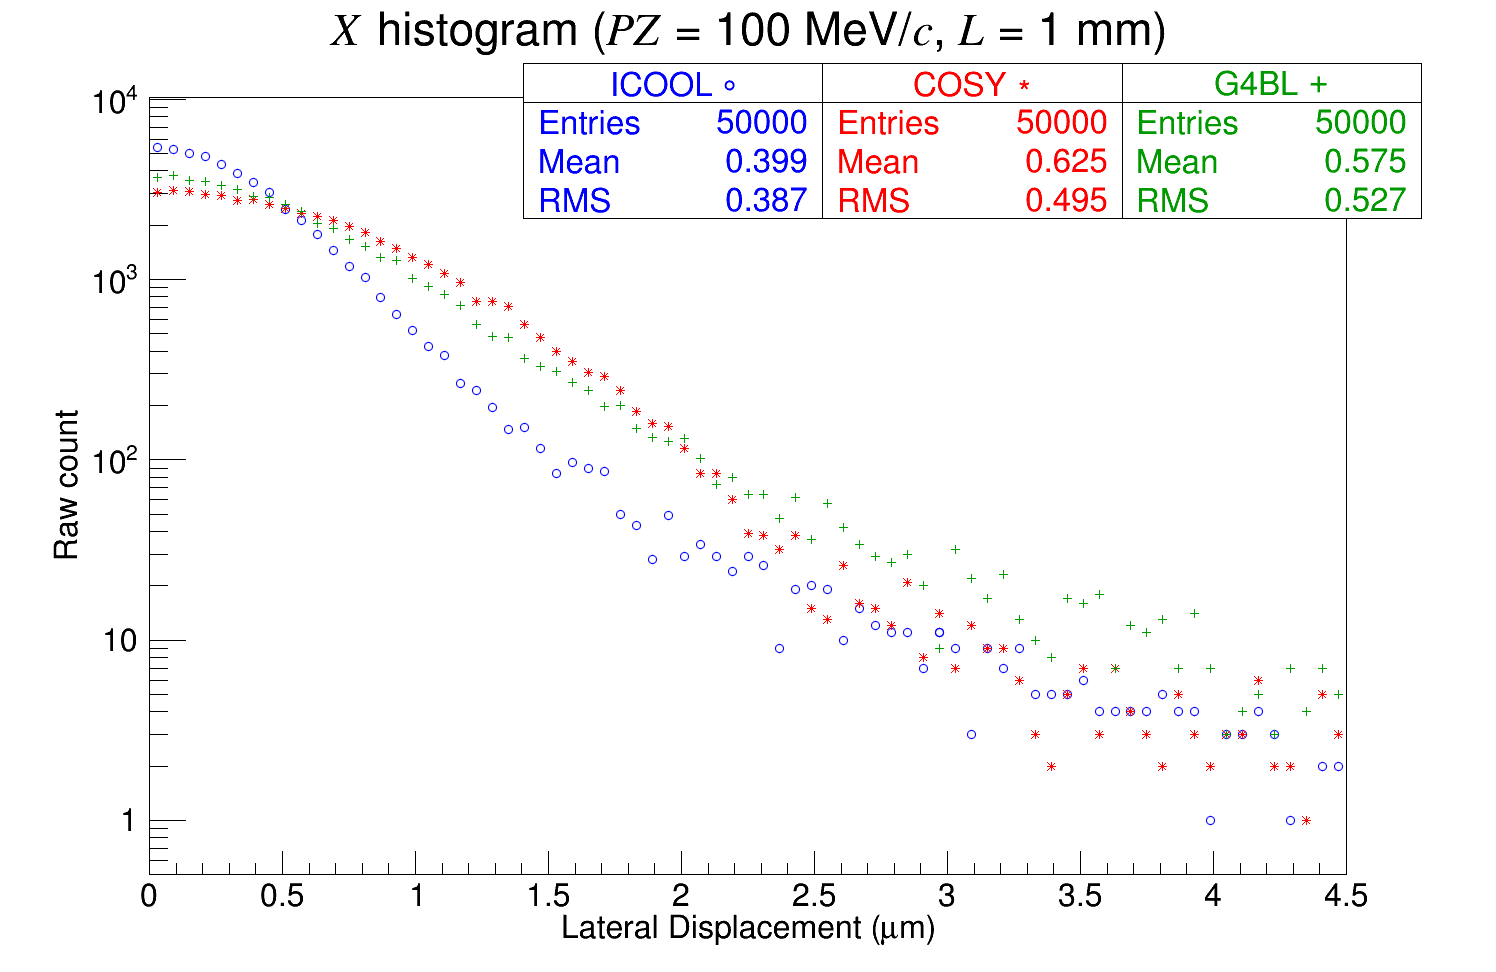
\includegraphics[width=0.7\textwidth]{Benchmarking/LH/X.100.1.png} 
    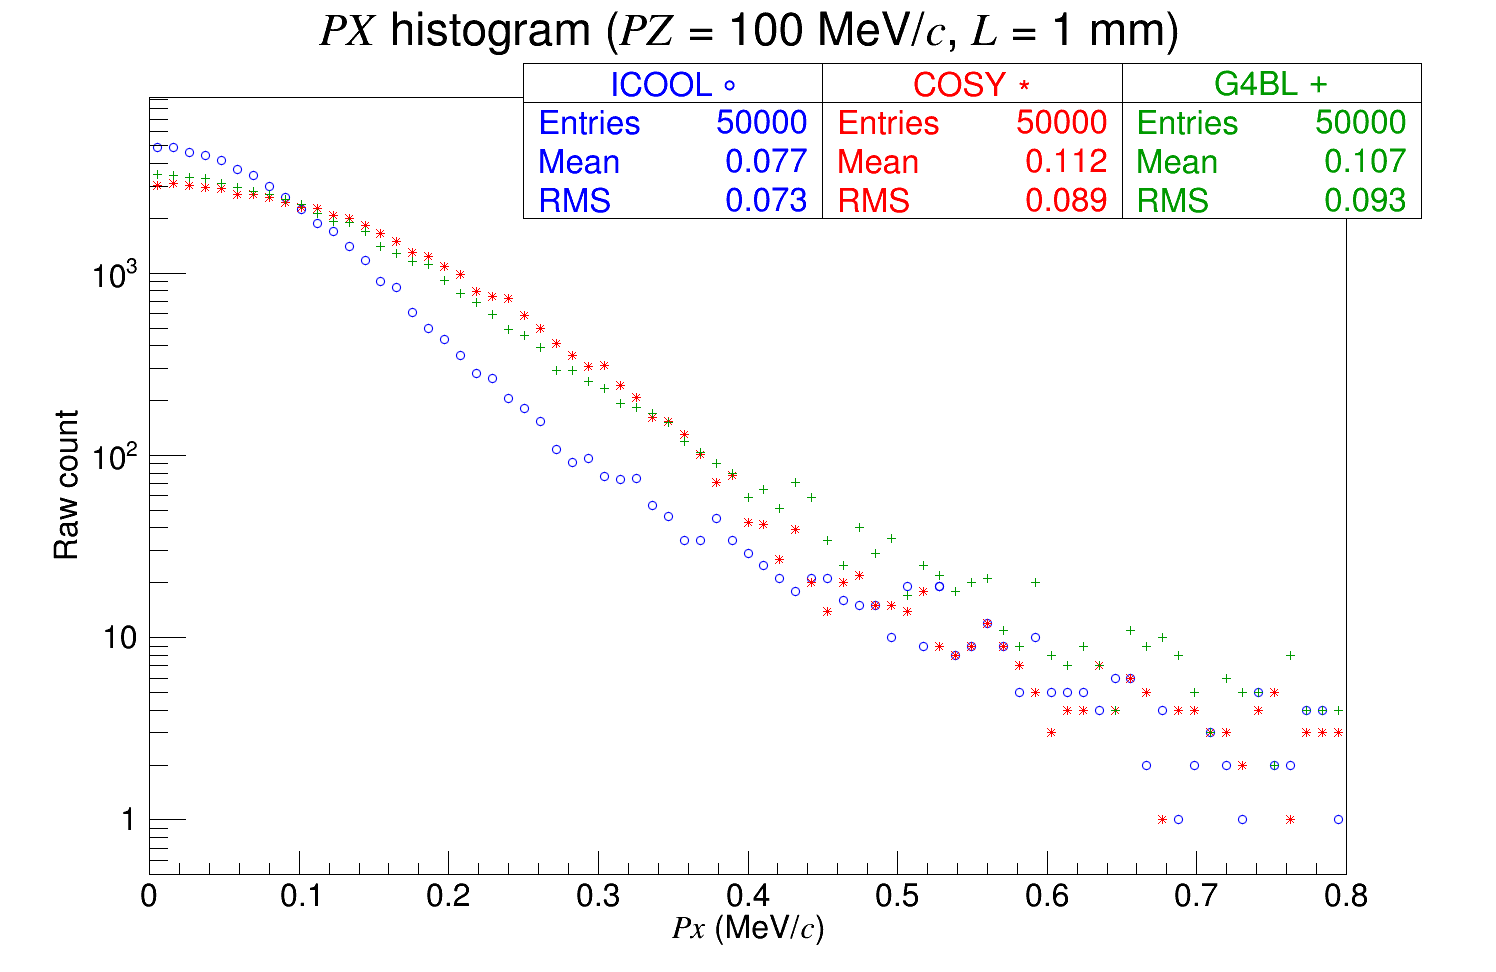
\includegraphics[width=0.7\textwidth]{Benchmarking/LH/PX.100.1.png} 
    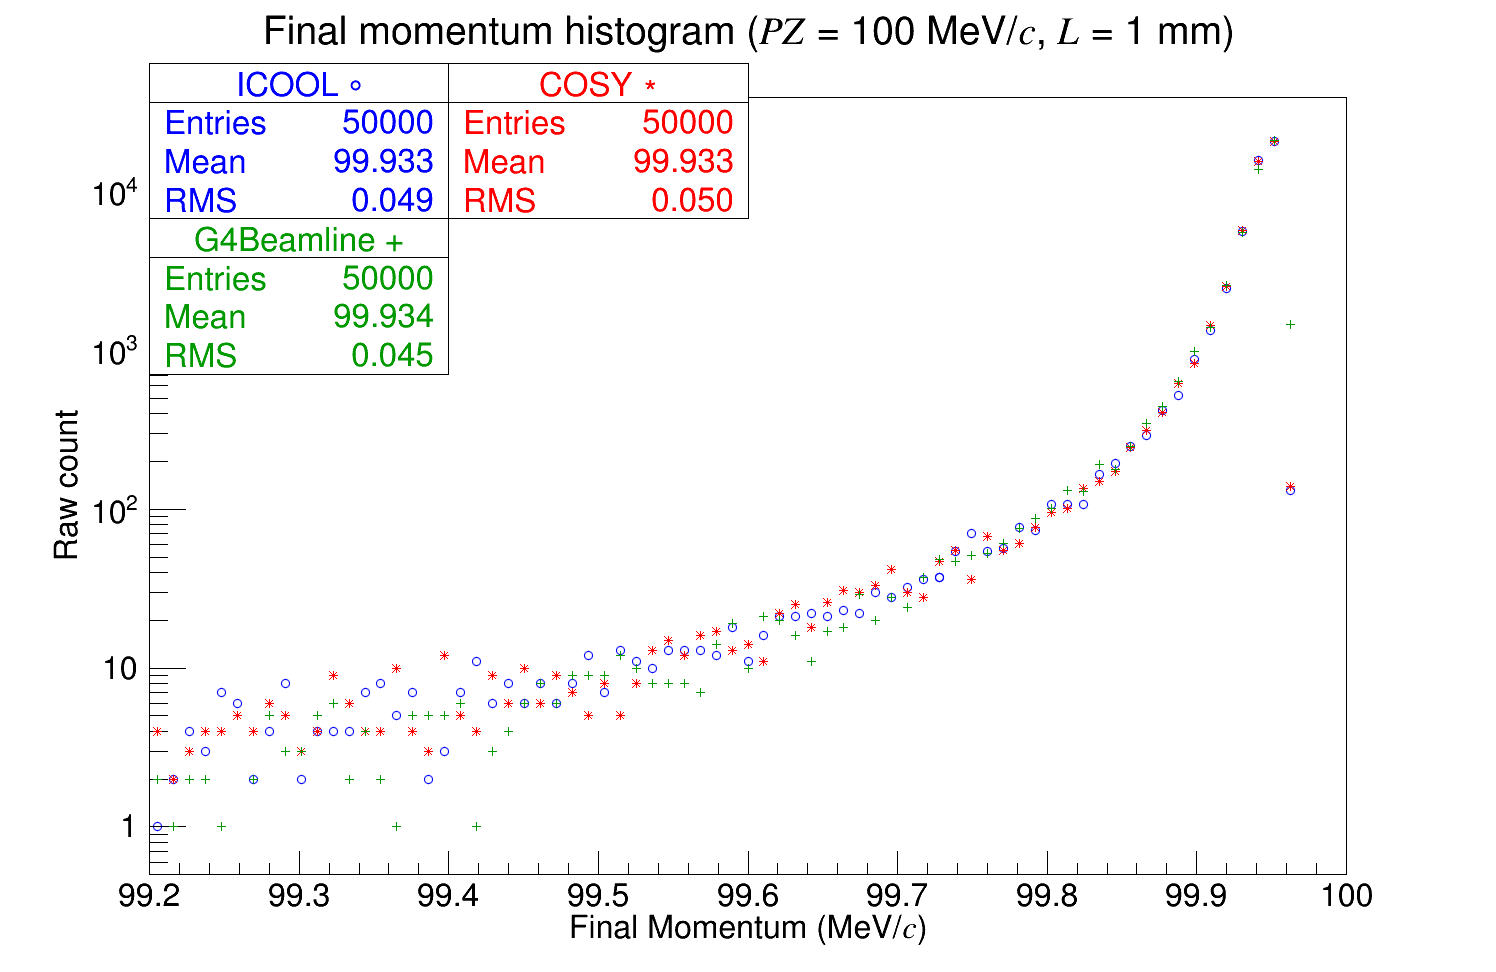
\includegraphics[width=0.7\textwidth]{Benchmarking/LH/strag.100.1.png} 
  \caption[Muons of momentum 100 MeV/$c$ through 1 mm liquid hydrogen.]{Muons of momentum 100 MeV/$c$ through 1 mm liquid hydrogen. Observe that for the $x$ and $p_x$ histograms, COSY and G4Beamline follow a Gaussian-like peak whereas ICOOL follows a Fano peak.}
  \label{fig:100.1}
\end{figure}

\begin{figure}[H]
  \centering
    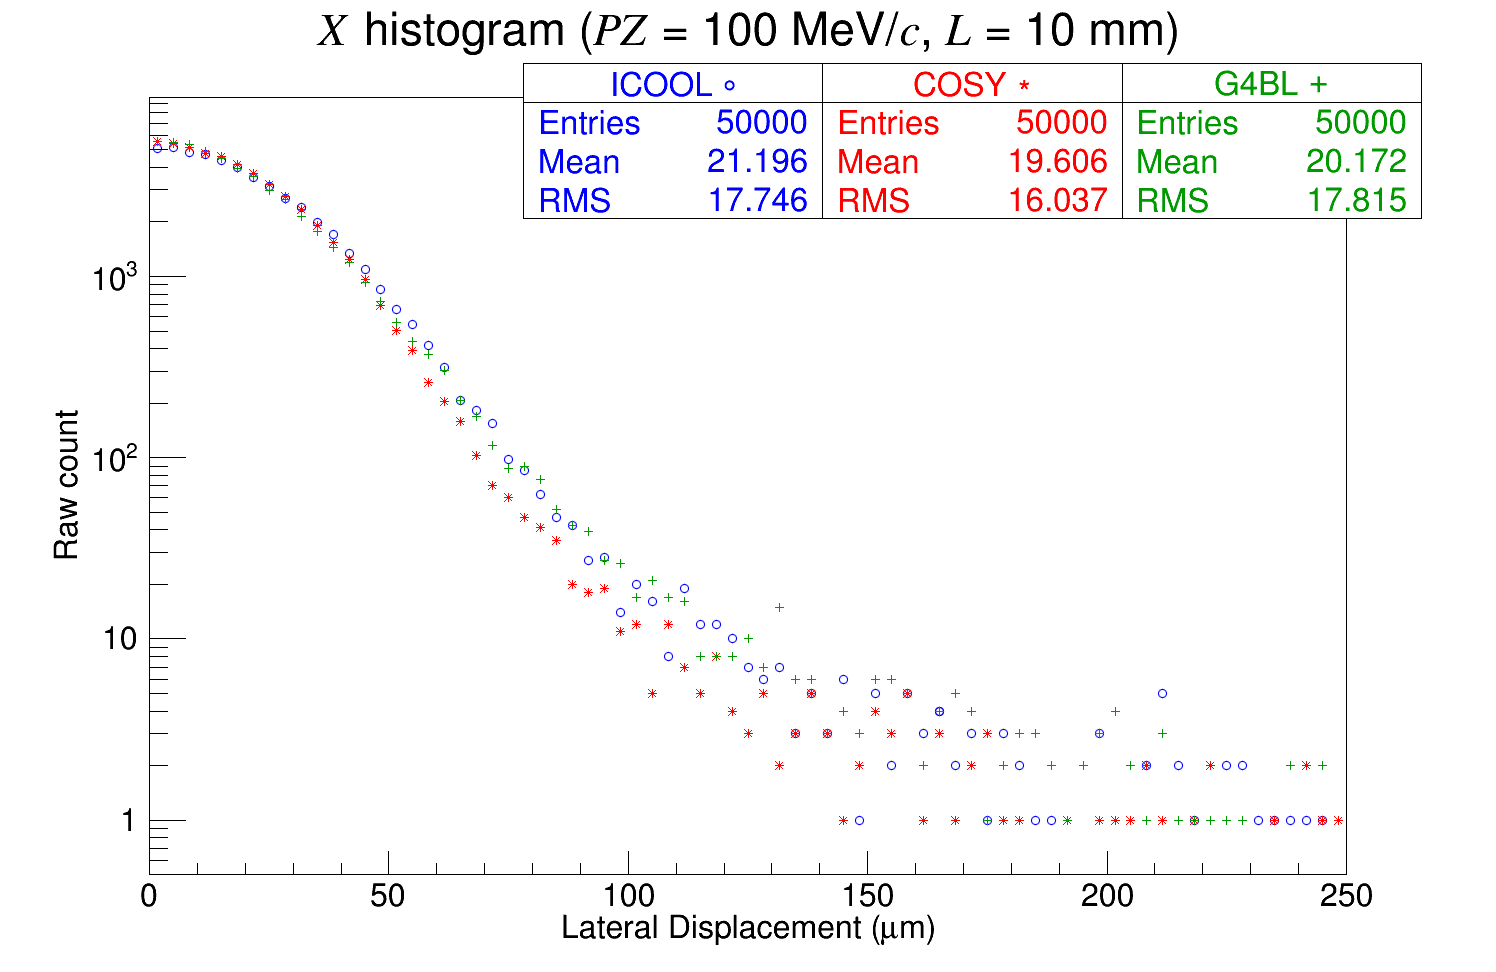
\includegraphics[width=0.7\textwidth]{Benchmarking/LH/X.100.10.png} 
    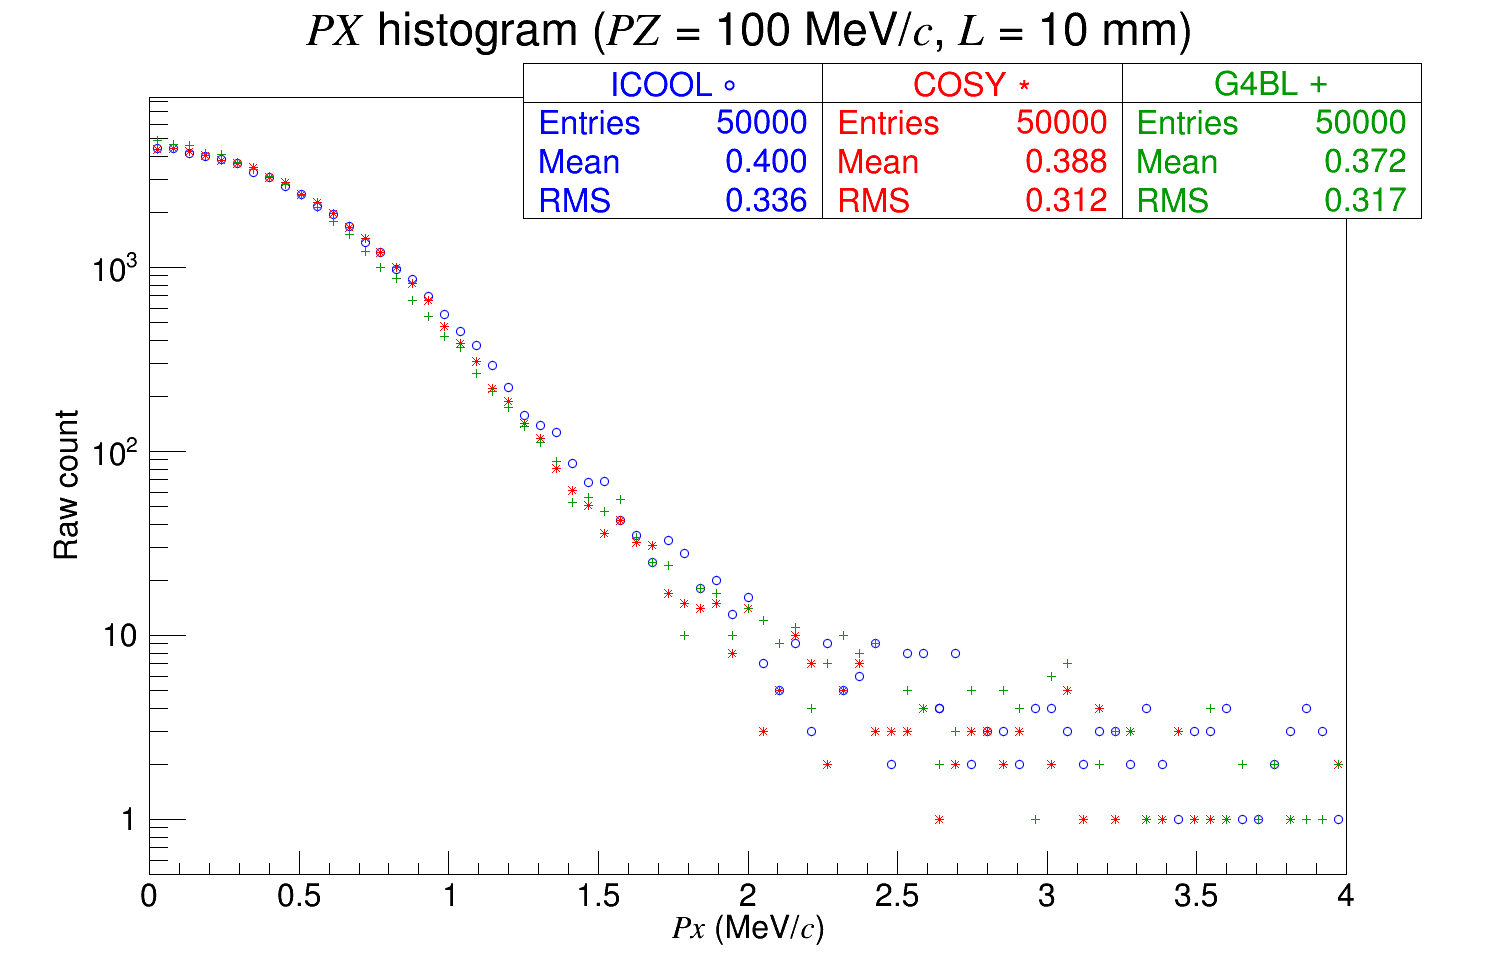
\includegraphics[width=0.7\textwidth]{Benchmarking/LH/PX.100.10.png} 
    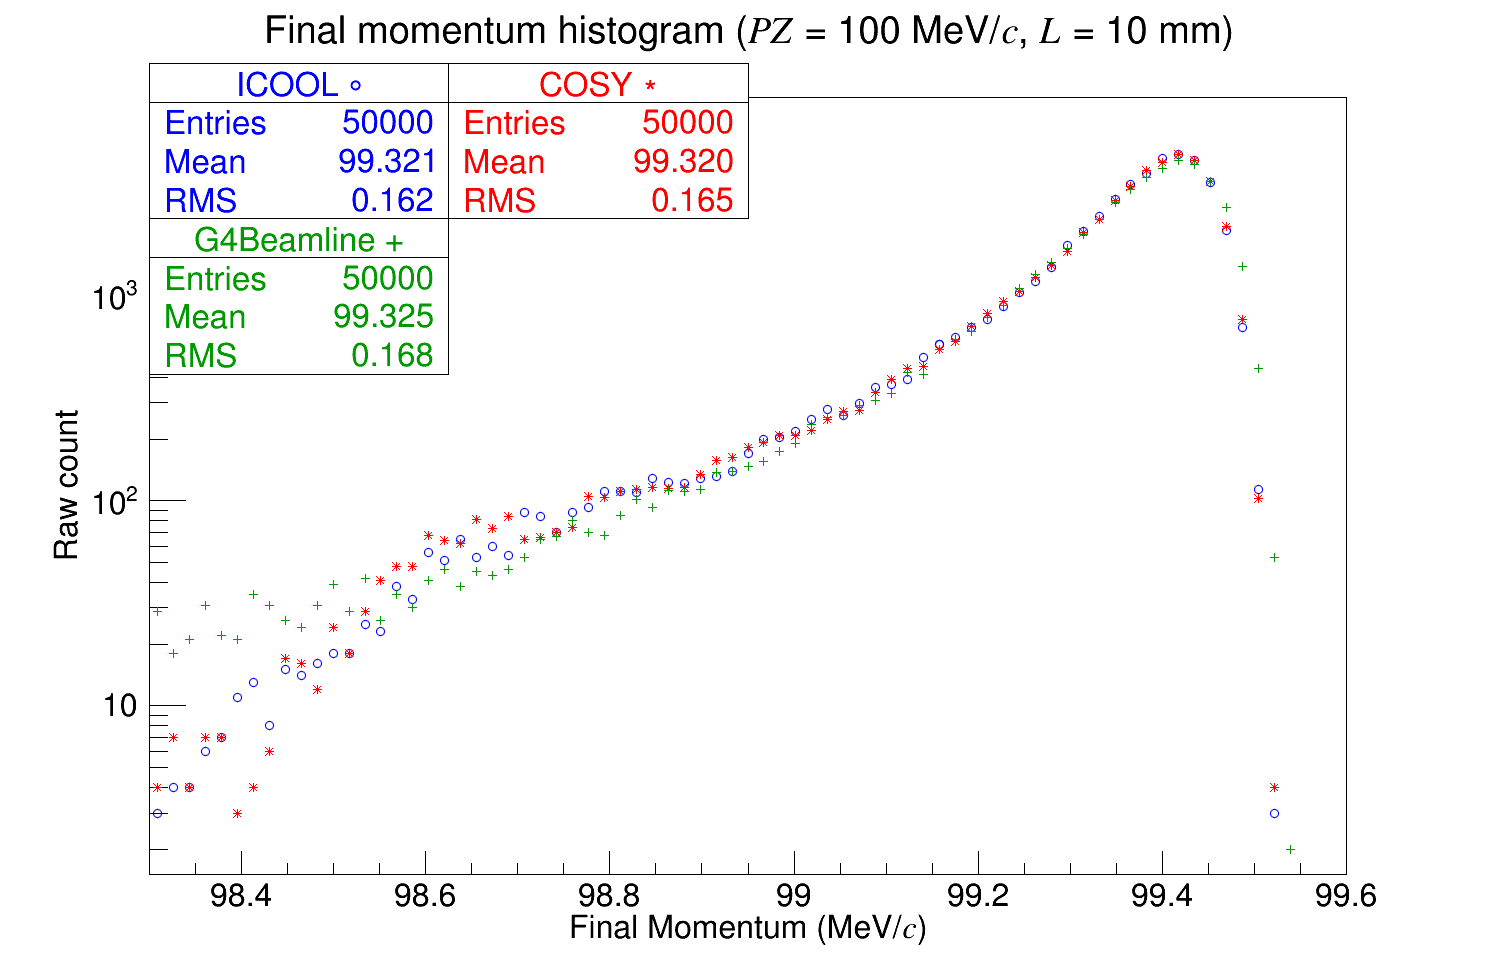
\includegraphics[width=0.7\textwidth]{Benchmarking/LH/strag.100.10.png} 
  \caption{Muons of momentum 100 MeV/$c$ through 10 mm liquid hydrogen.}
  \label{fig:100.10}
\end{figure}

\begin{figure}[H]
  \centering
    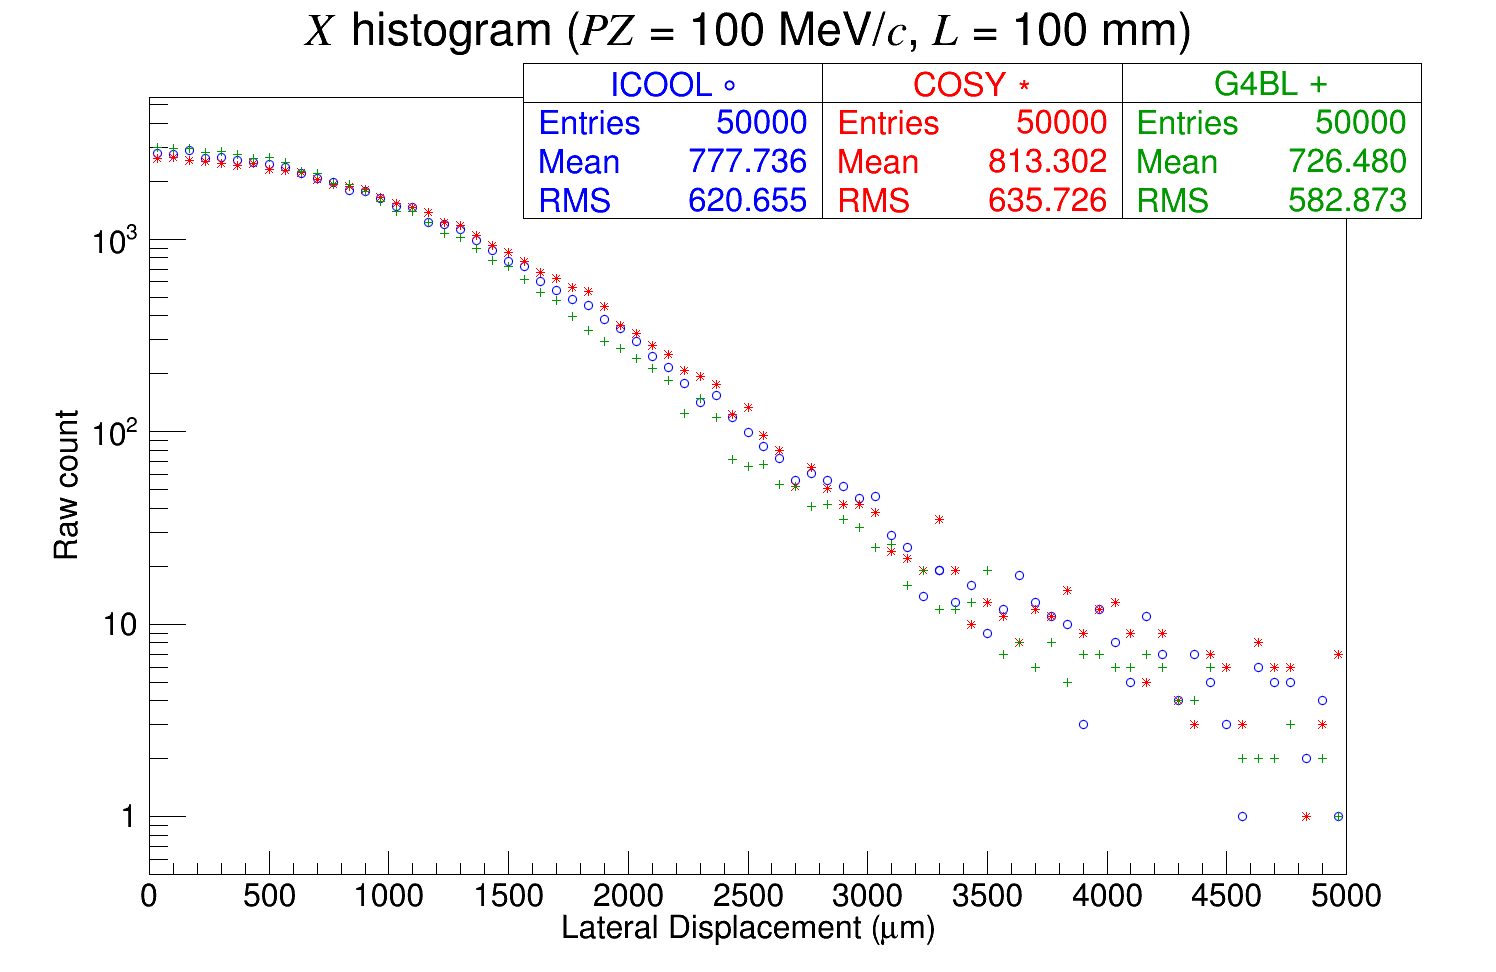
\includegraphics[width=0.7\textwidth]{Benchmarking/LH/X.100.100.png} 
    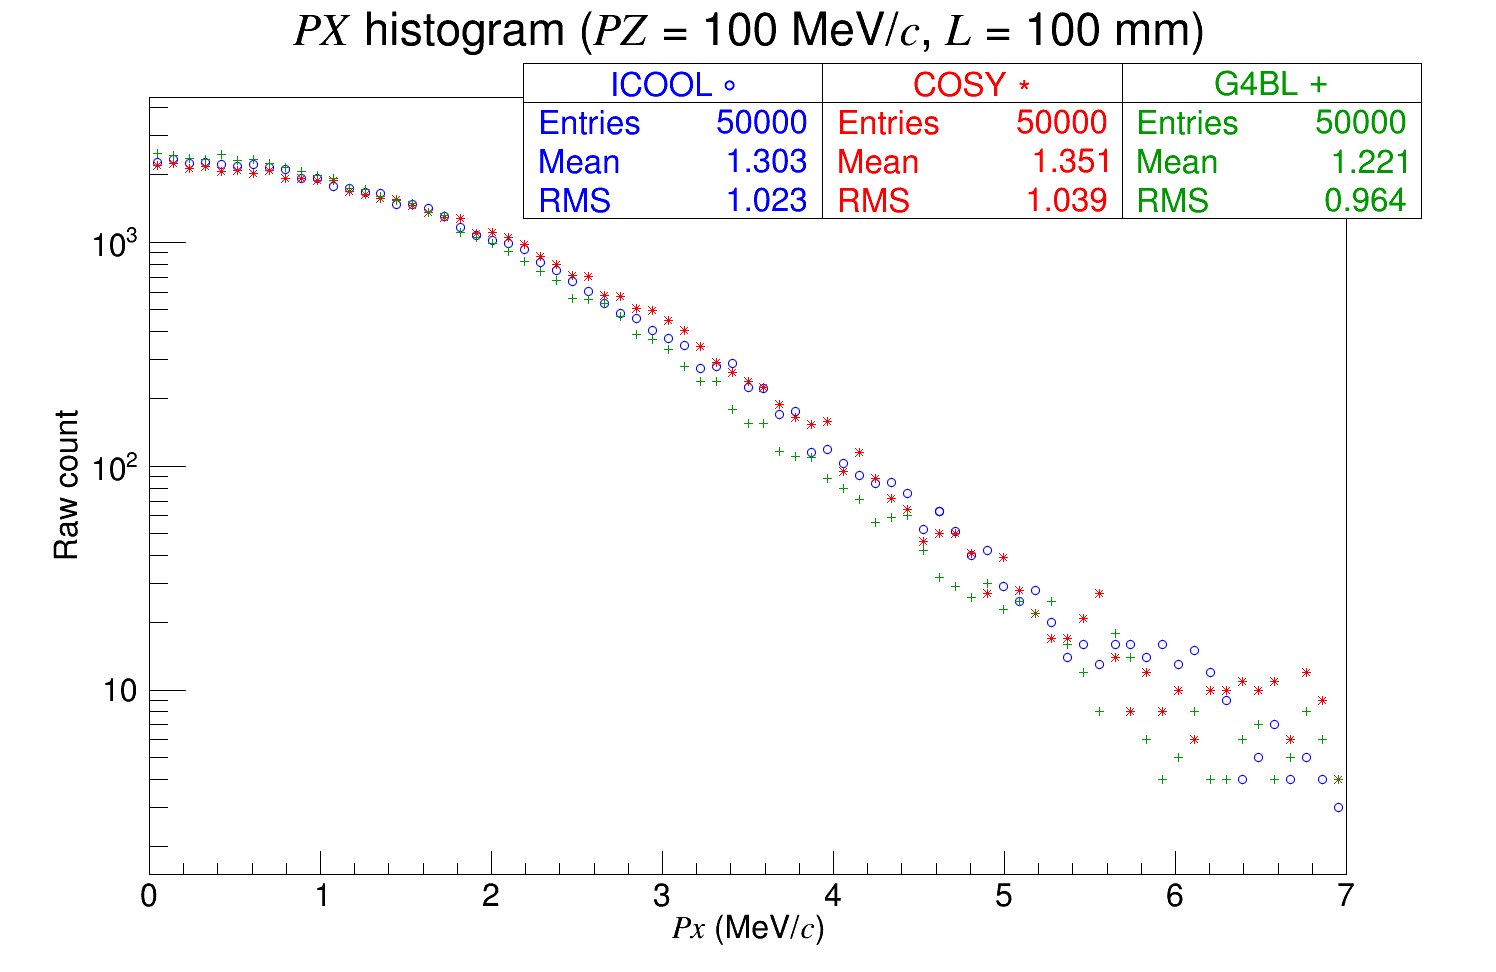
\includegraphics[width=0.7\textwidth]{Benchmarking/LH/PX.100.100.png} 
    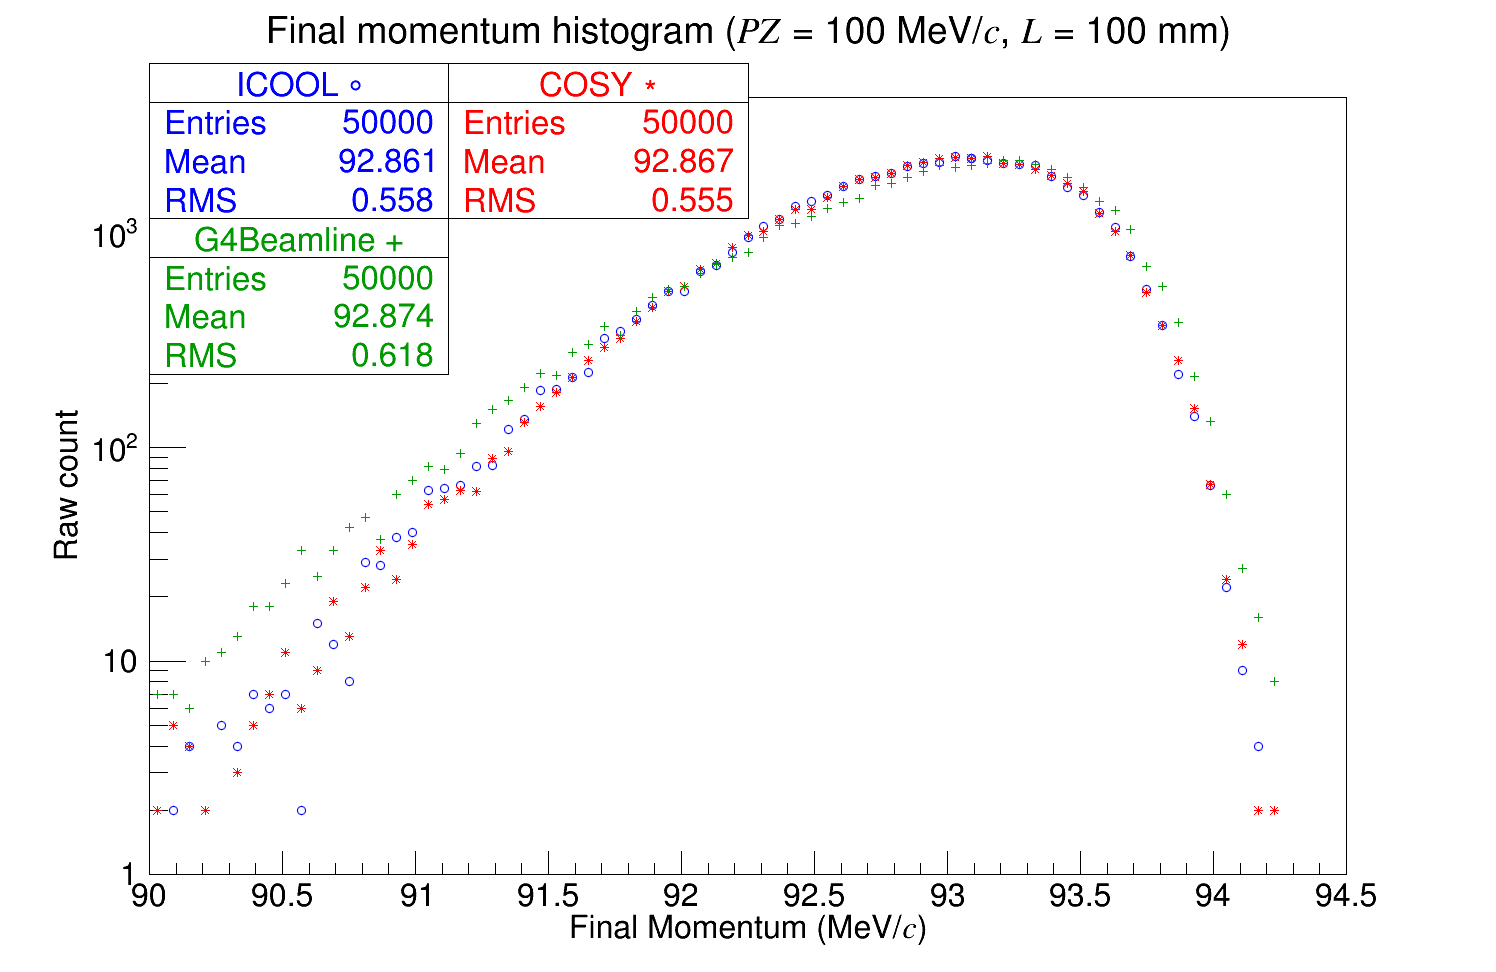
\includegraphics[width=0.7\textwidth]{Benchmarking/LH/strag.100.100.png} 
  \caption{Muons of momentum 100 MeV/$c$ through 100 mm liquid hydrogen.}
  \label{fig:100.100}
\end{figure}

\begin{figure}[H]
  \centering
    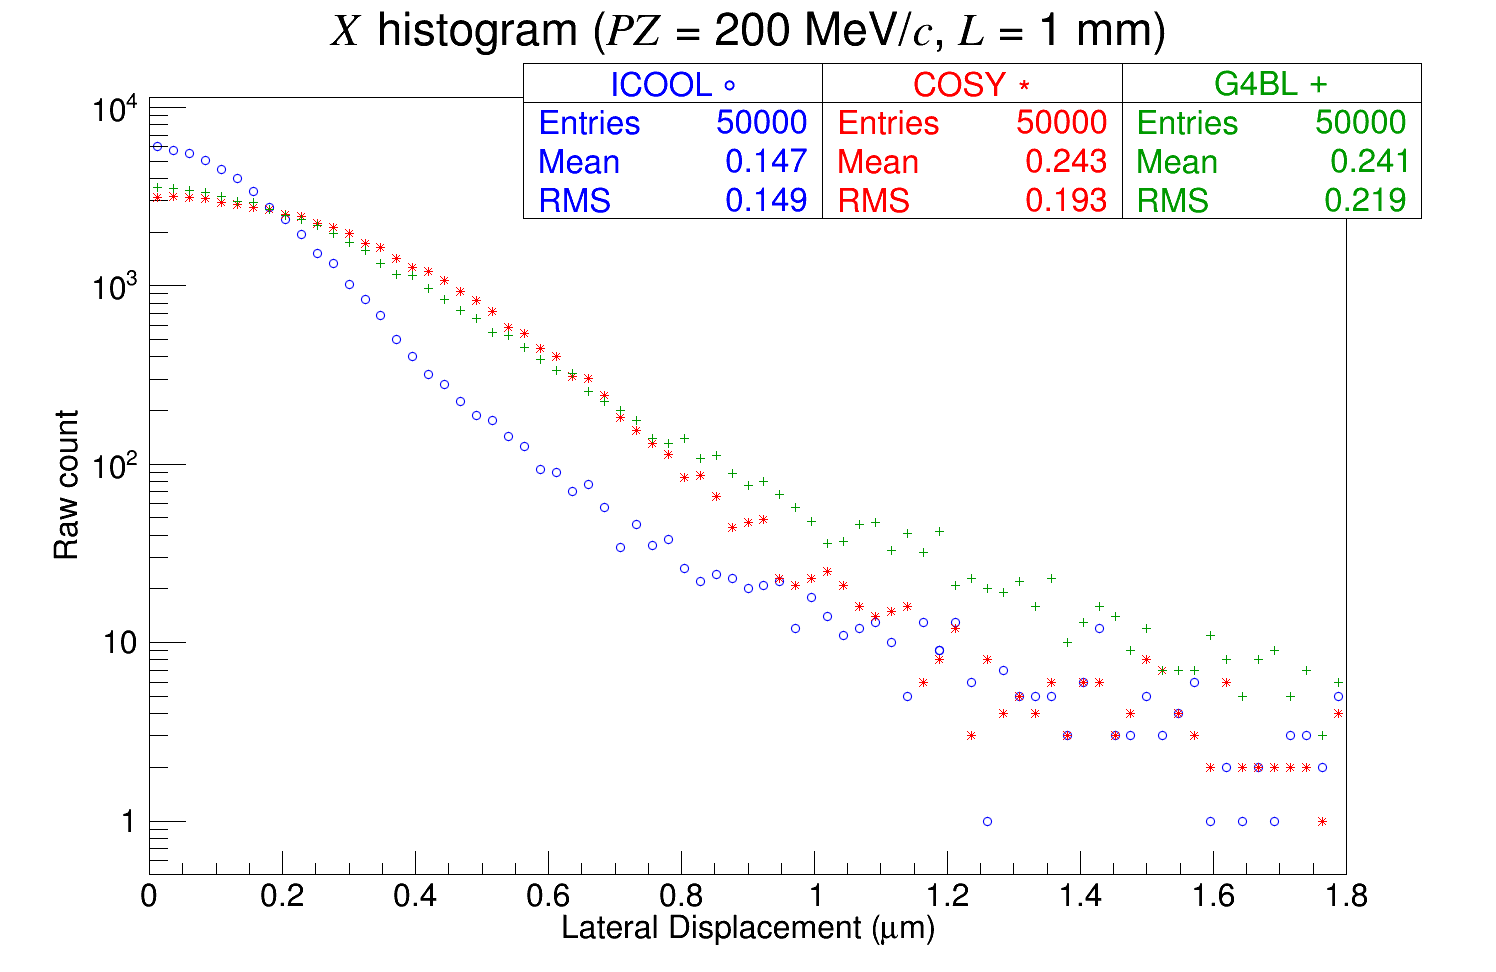
\includegraphics[width=0.7\textwidth]{Benchmarking/LH/X.200.1.png} 
    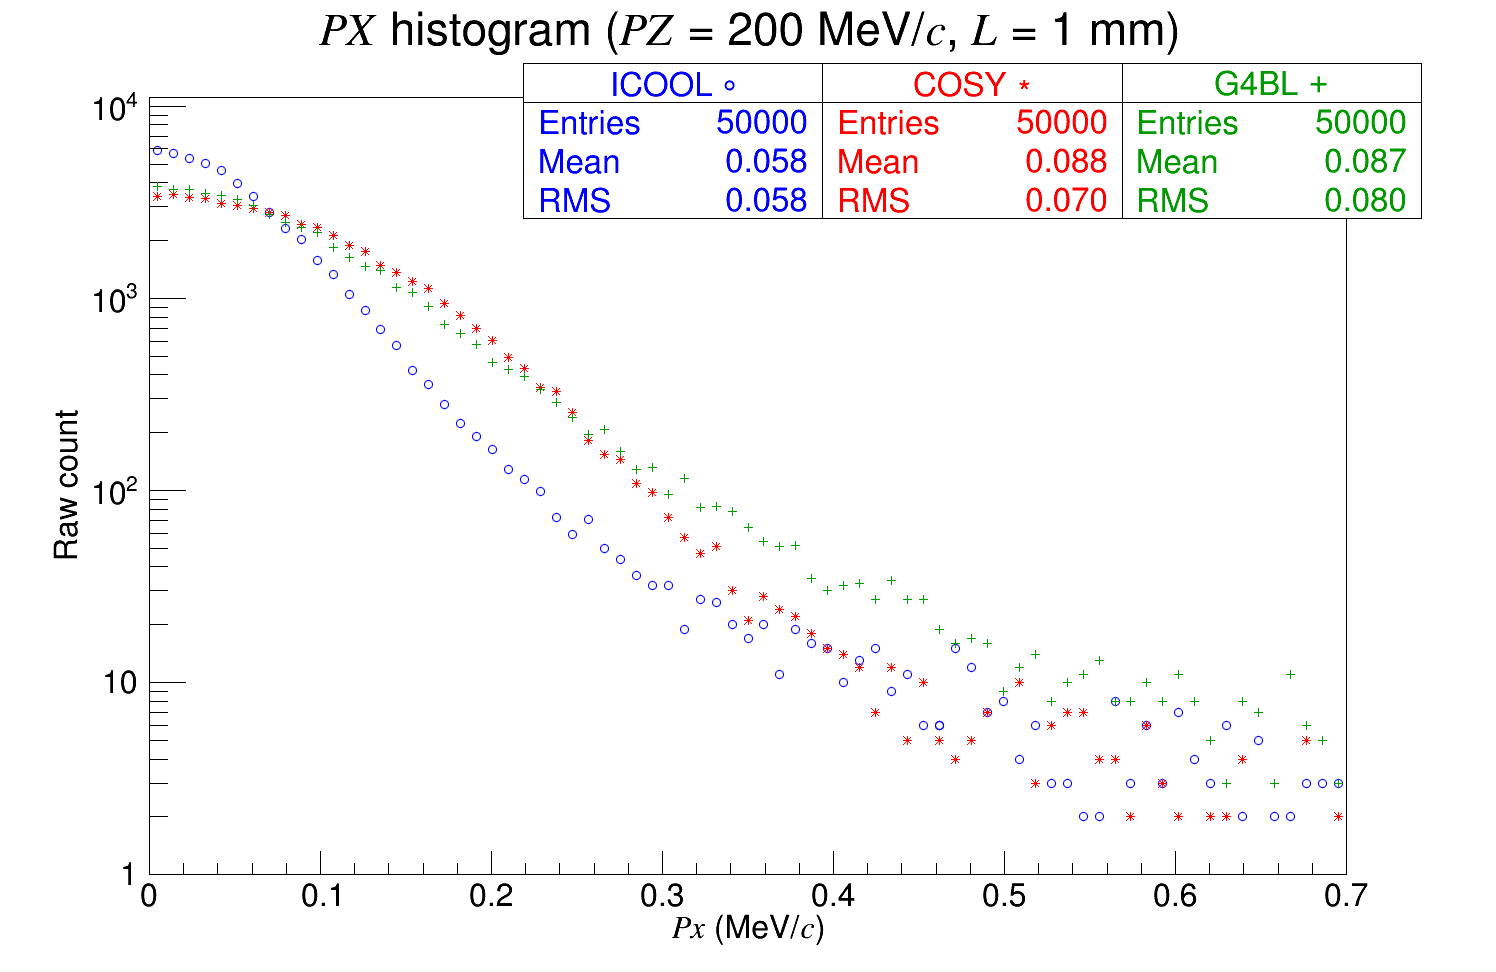
\includegraphics[width=0.7\textwidth]{Benchmarking/LH/PX.200.1.png} 
    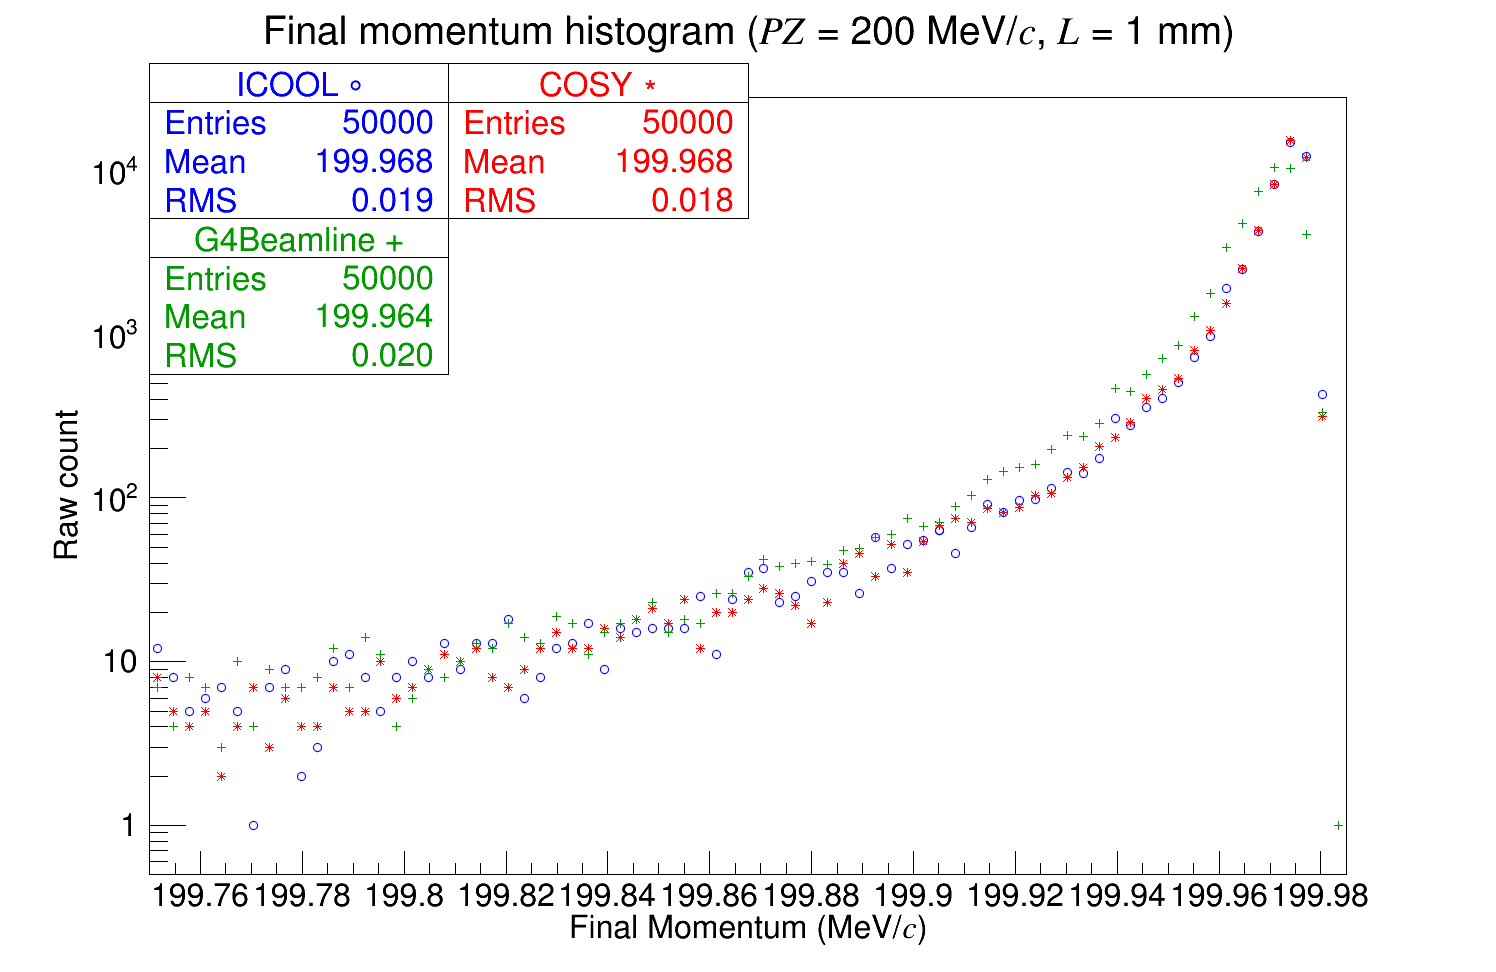
\includegraphics[width=0.7\textwidth]{Benchmarking/LH/strag.200.1.png} 
  \caption[Muons of momentum 200 MeV/$c$ through 1 mm liquid hydrogen.]{Muons of momentum 100 MeV/$c$ through 1 mm liquid hydrogen. Observe that for the $x$ and $p_x$ histograms, COSY and G4Beamline follow a Gaussian-like peak whereas ICOOL follows a Fano peak.}
  \label{fig:200.1}
\end{figure}

\begin{figure}[H]
  \centering
    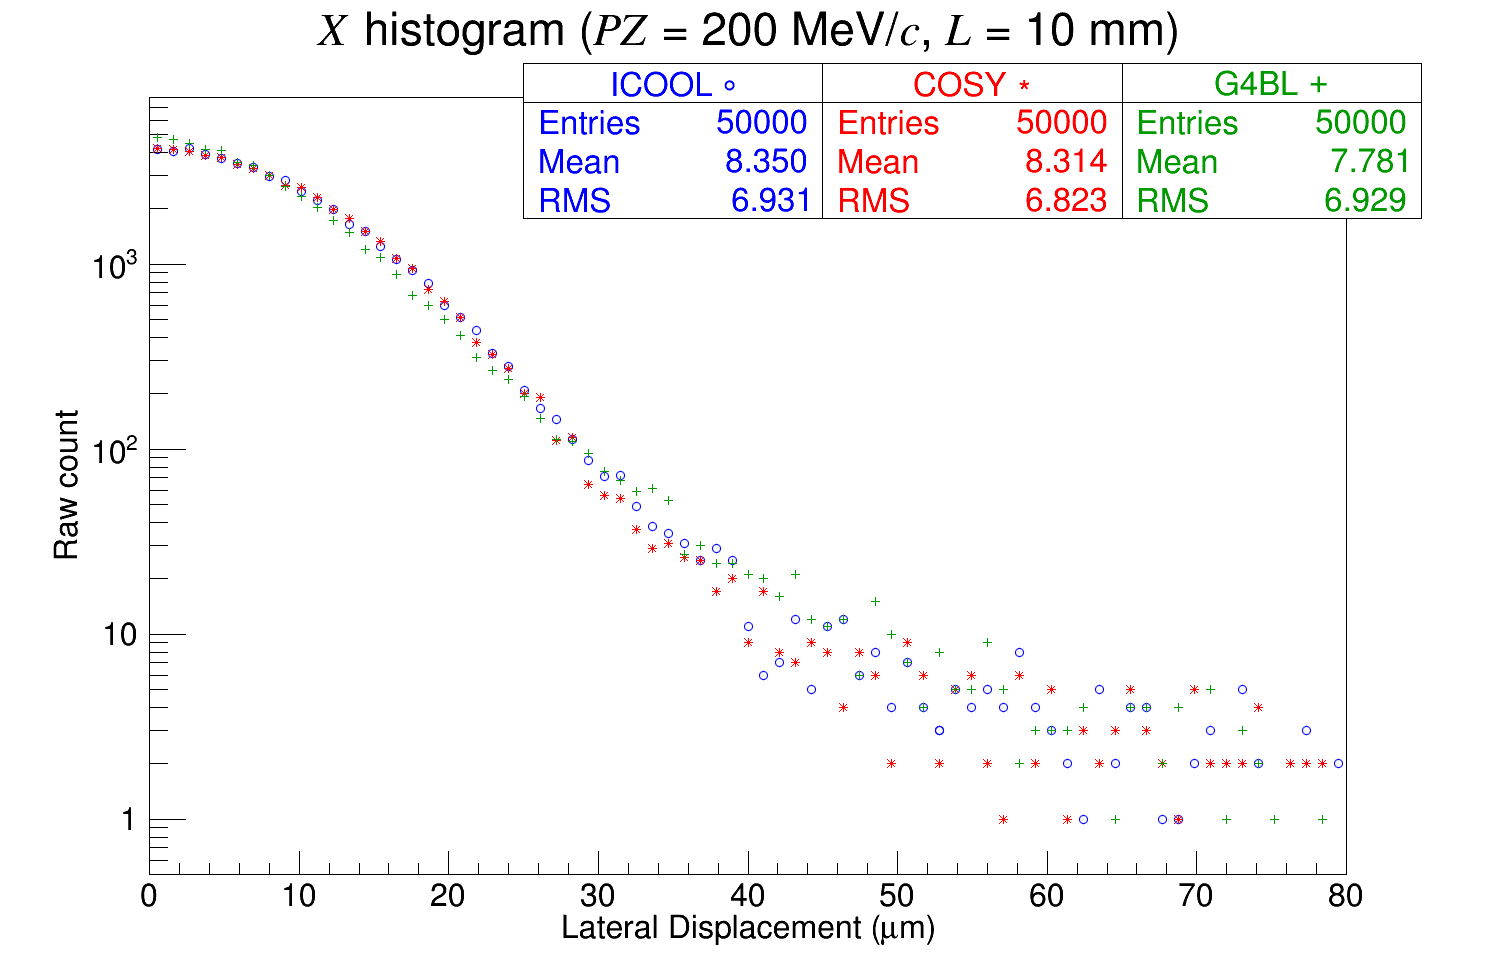
\includegraphics[width=0.7\textwidth]{Benchmarking/LH/X.200.10.png} 
    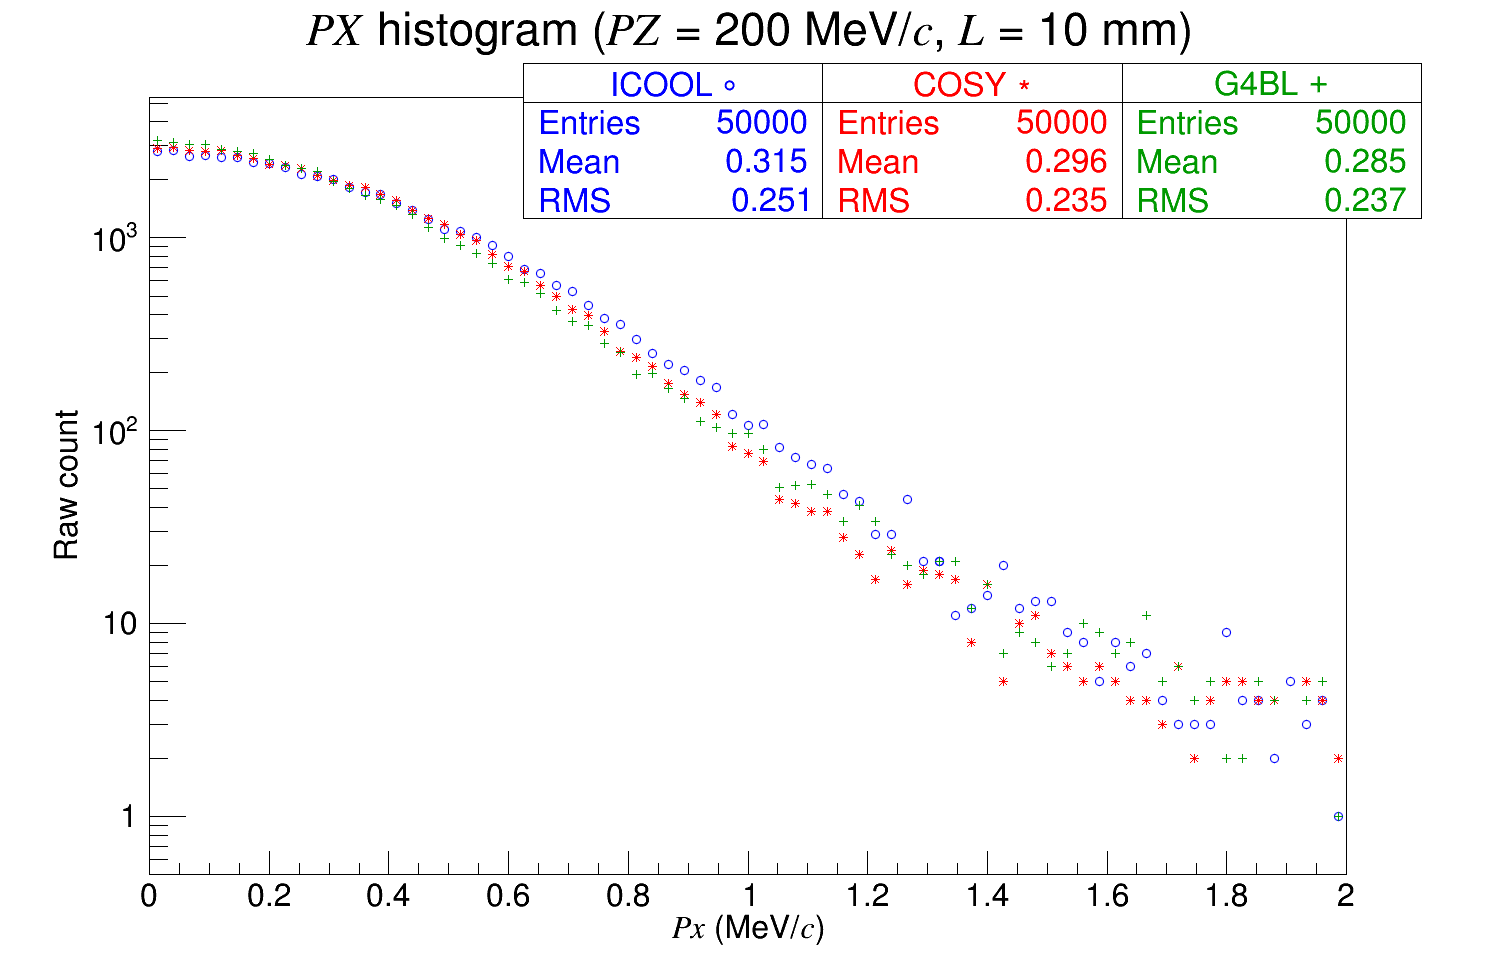
\includegraphics[width=0.7\textwidth]{Benchmarking/LH/PX.200.10.png} 
    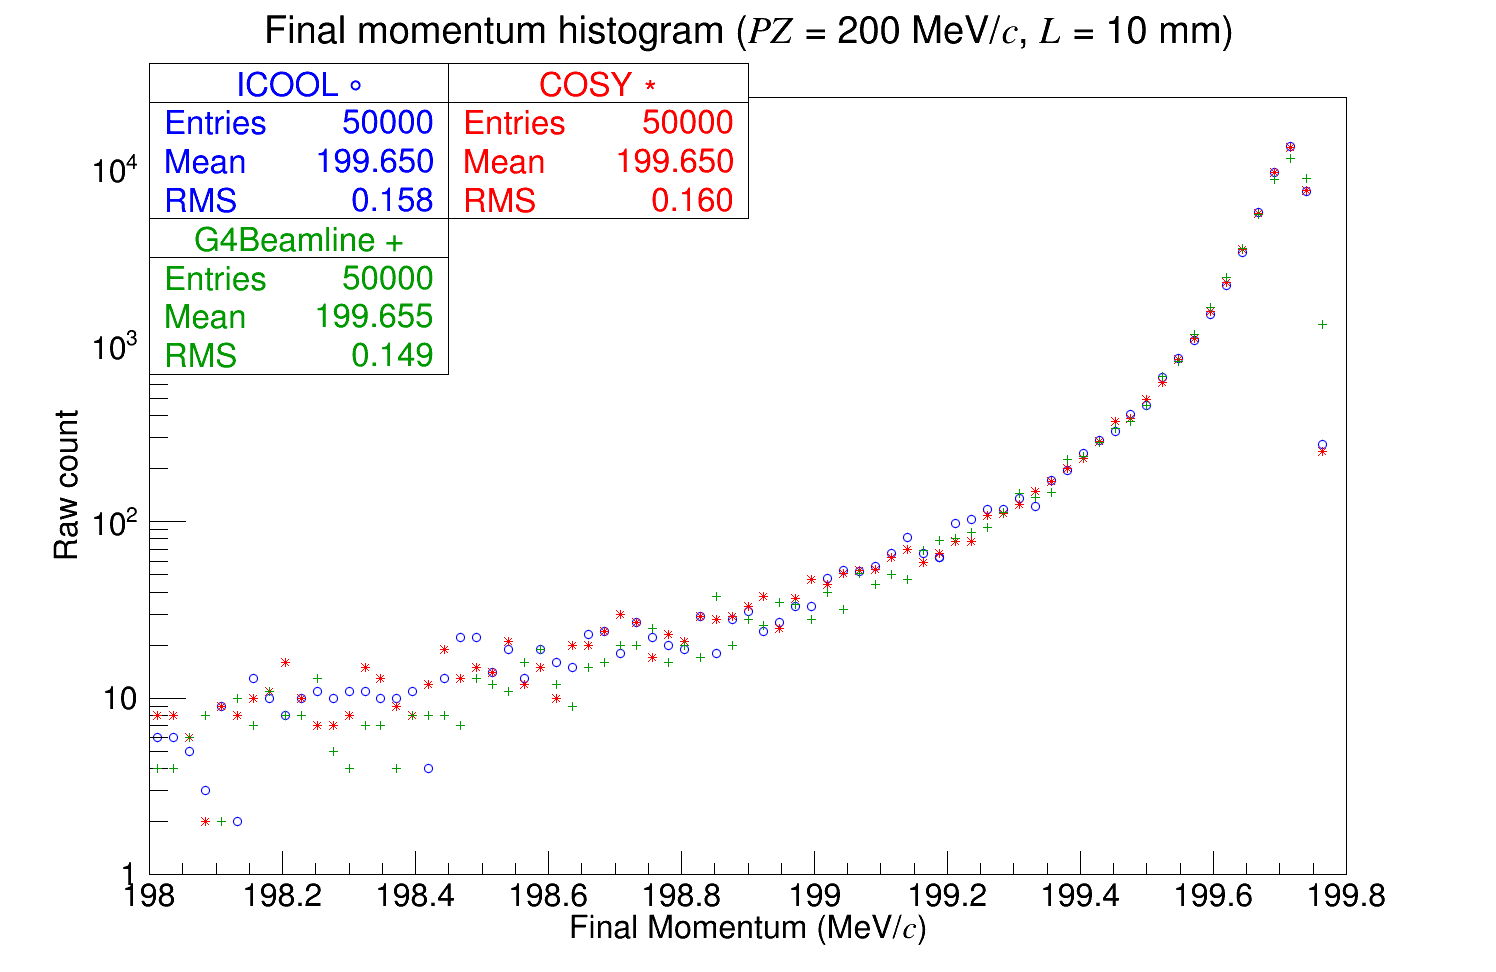
\includegraphics[width=0.7\textwidth]{Benchmarking/LH/strag.200.10.png} 
  \caption{Muons of momentum 200 MeV/$c$ through 10 mm liquid hydrogen.}
  \label{fig:200.10}
\end{figure}

\begin{figure}[H]
  \centering
    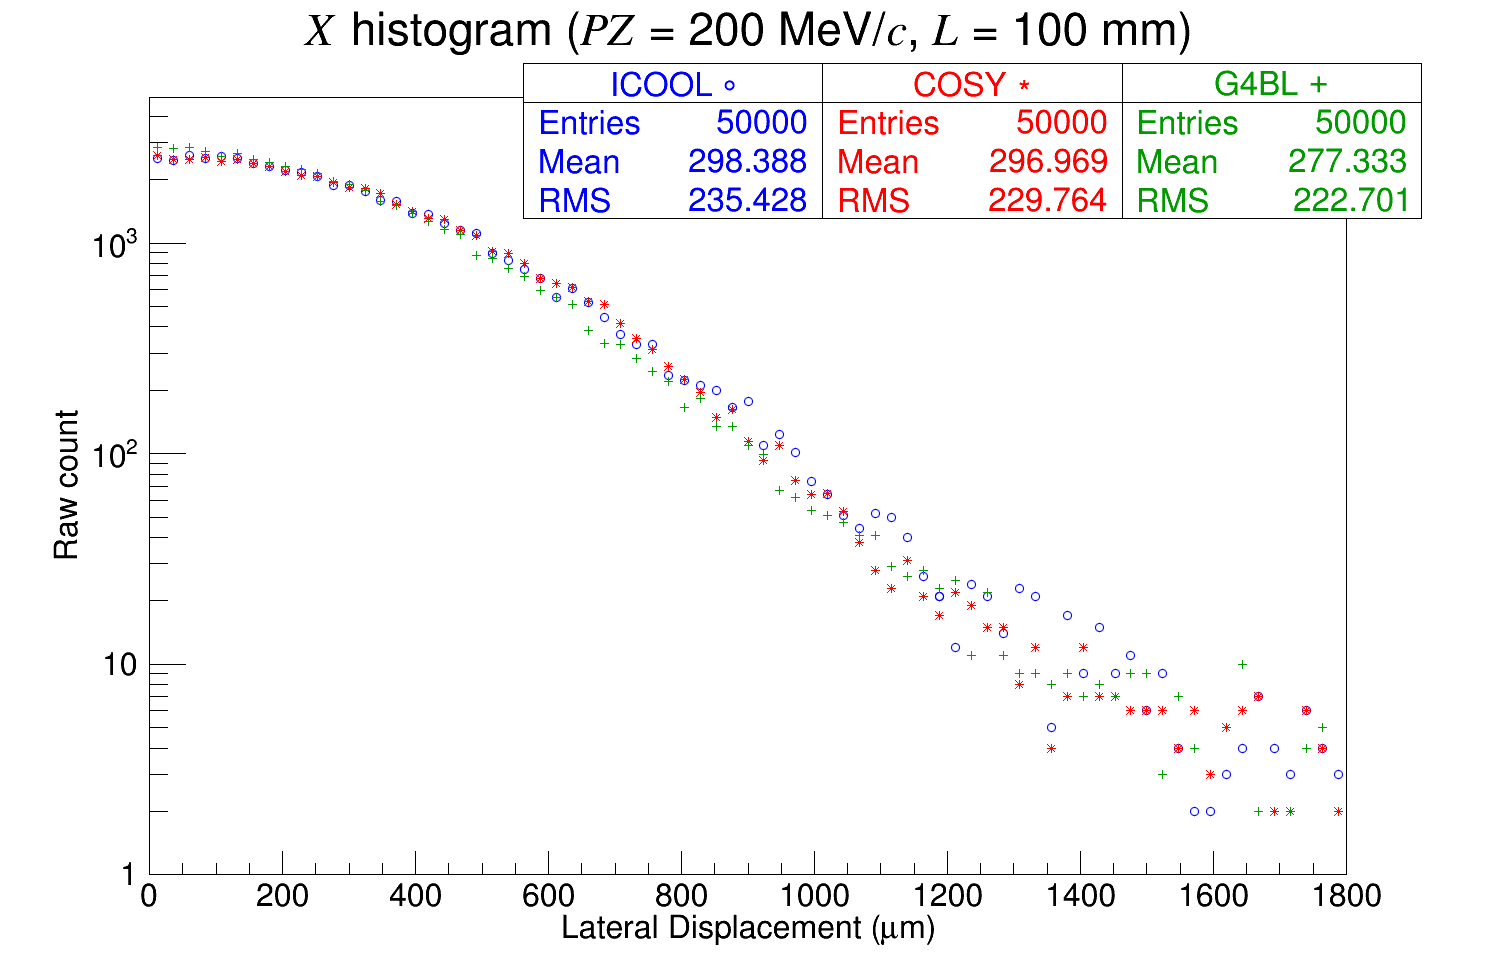
\includegraphics[width=0.7\textwidth]{Benchmarking/LH/X.200.100.png} 
    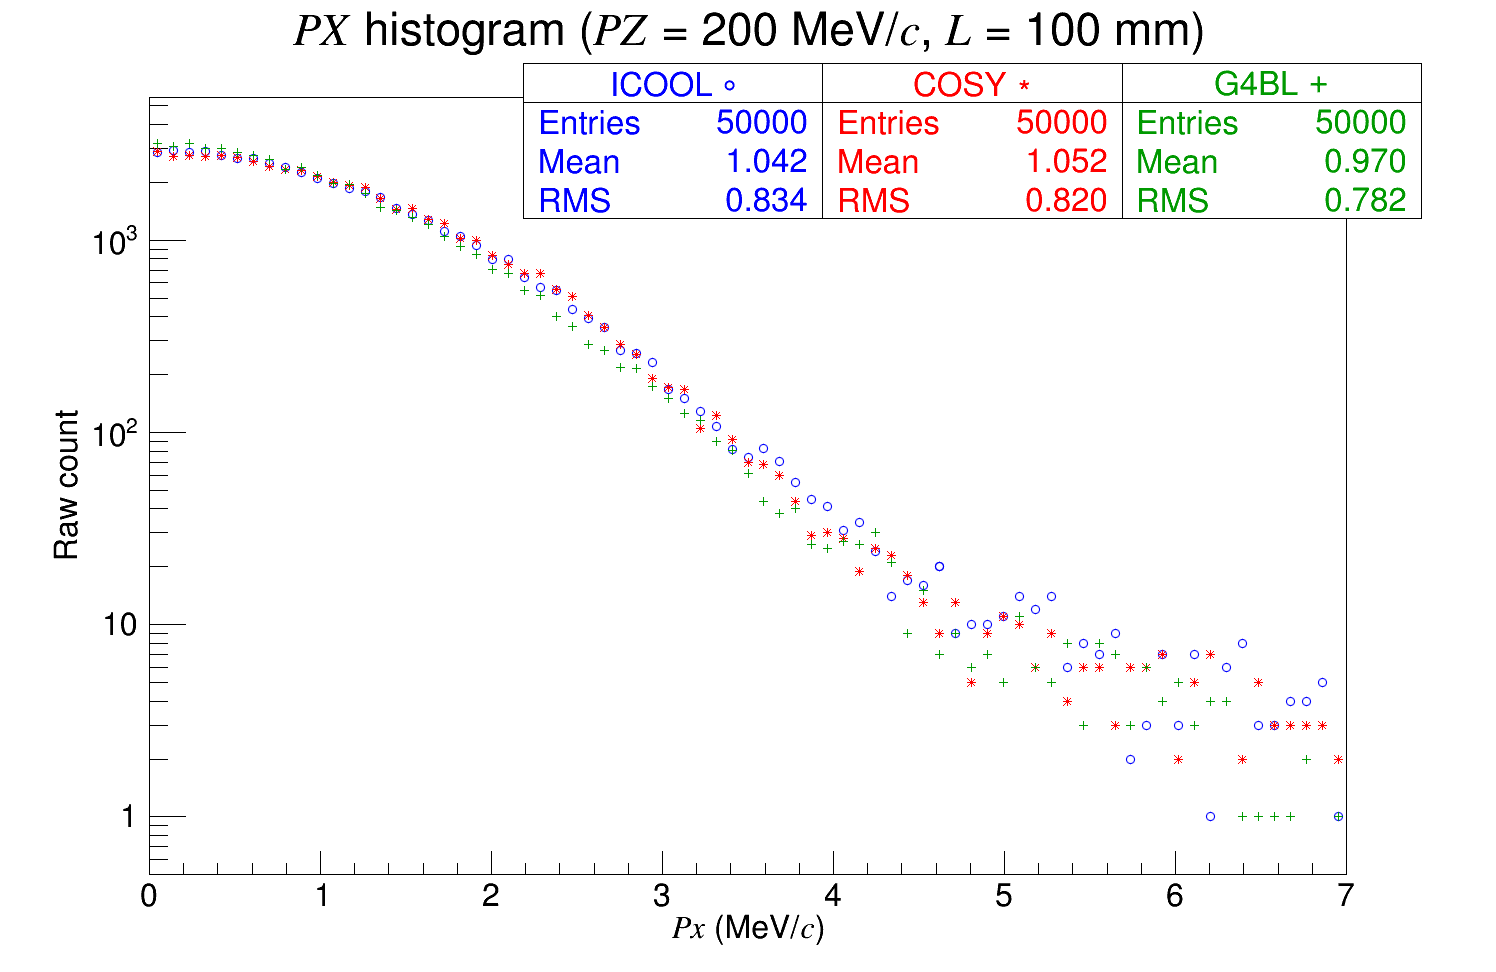
\includegraphics[width=0.7\textwidth]{Benchmarking/LH/PX.200.100.png} 
    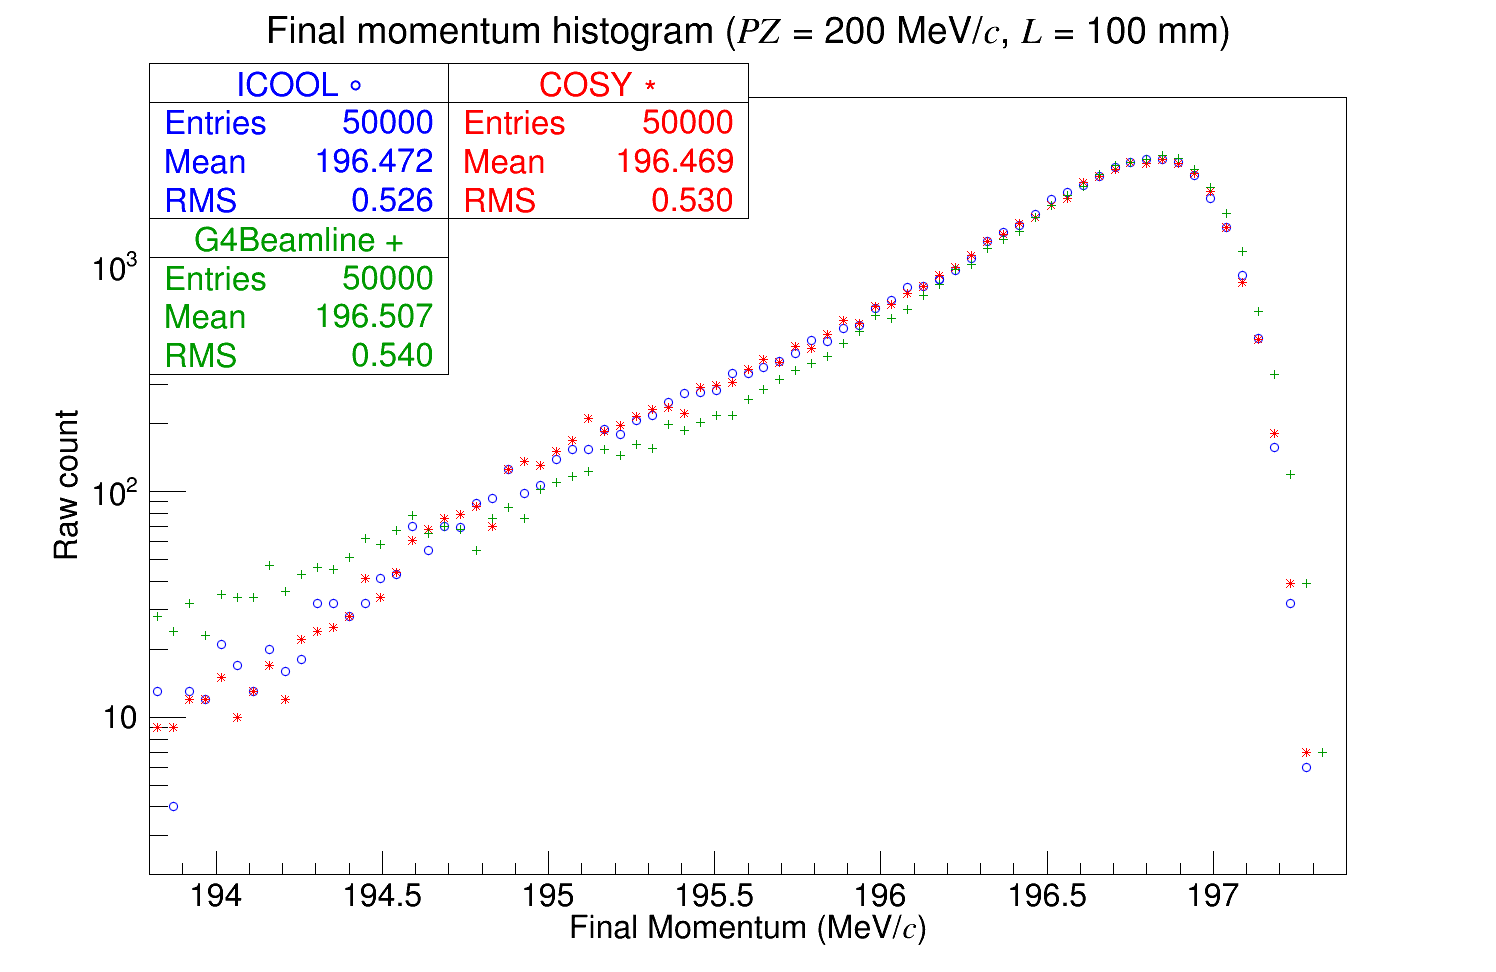
\includegraphics[width=0.7\textwidth]{Benchmarking/LH/strag.200.100.png} 
  \caption{Muons of momentum 200 MeV/$c$ through 100 mm liquid hydrogen.}
  \label{fig:200.100}
\end{figure}

\begin{figure}[H]
  \centering
    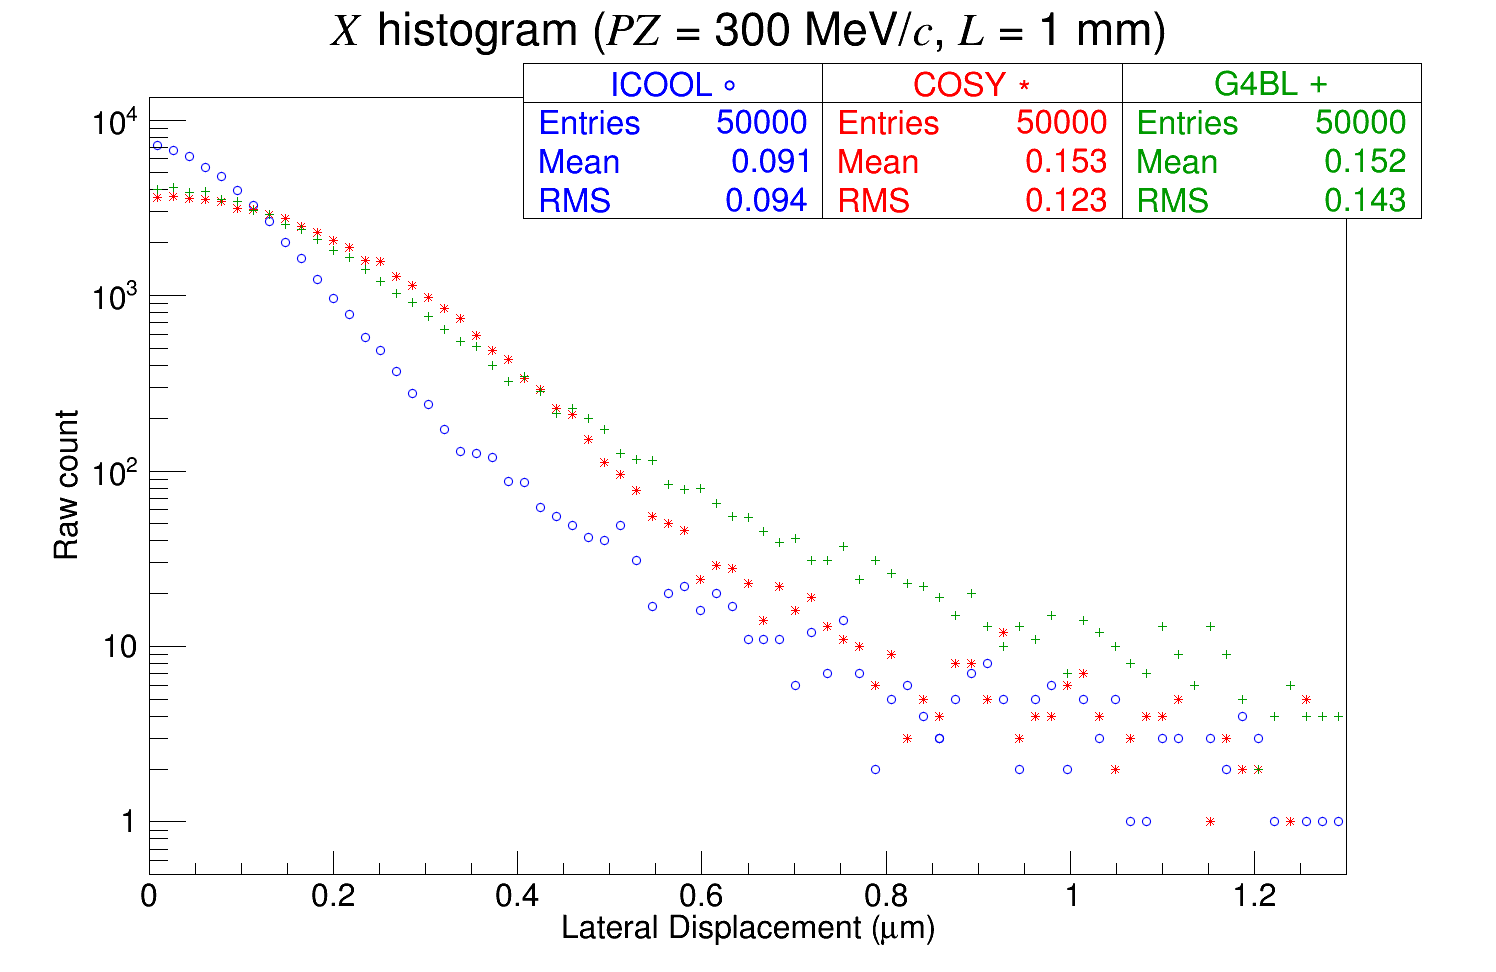
\includegraphics[width=0.7\textwidth]{Benchmarking/LH/X.300.1.png} 
    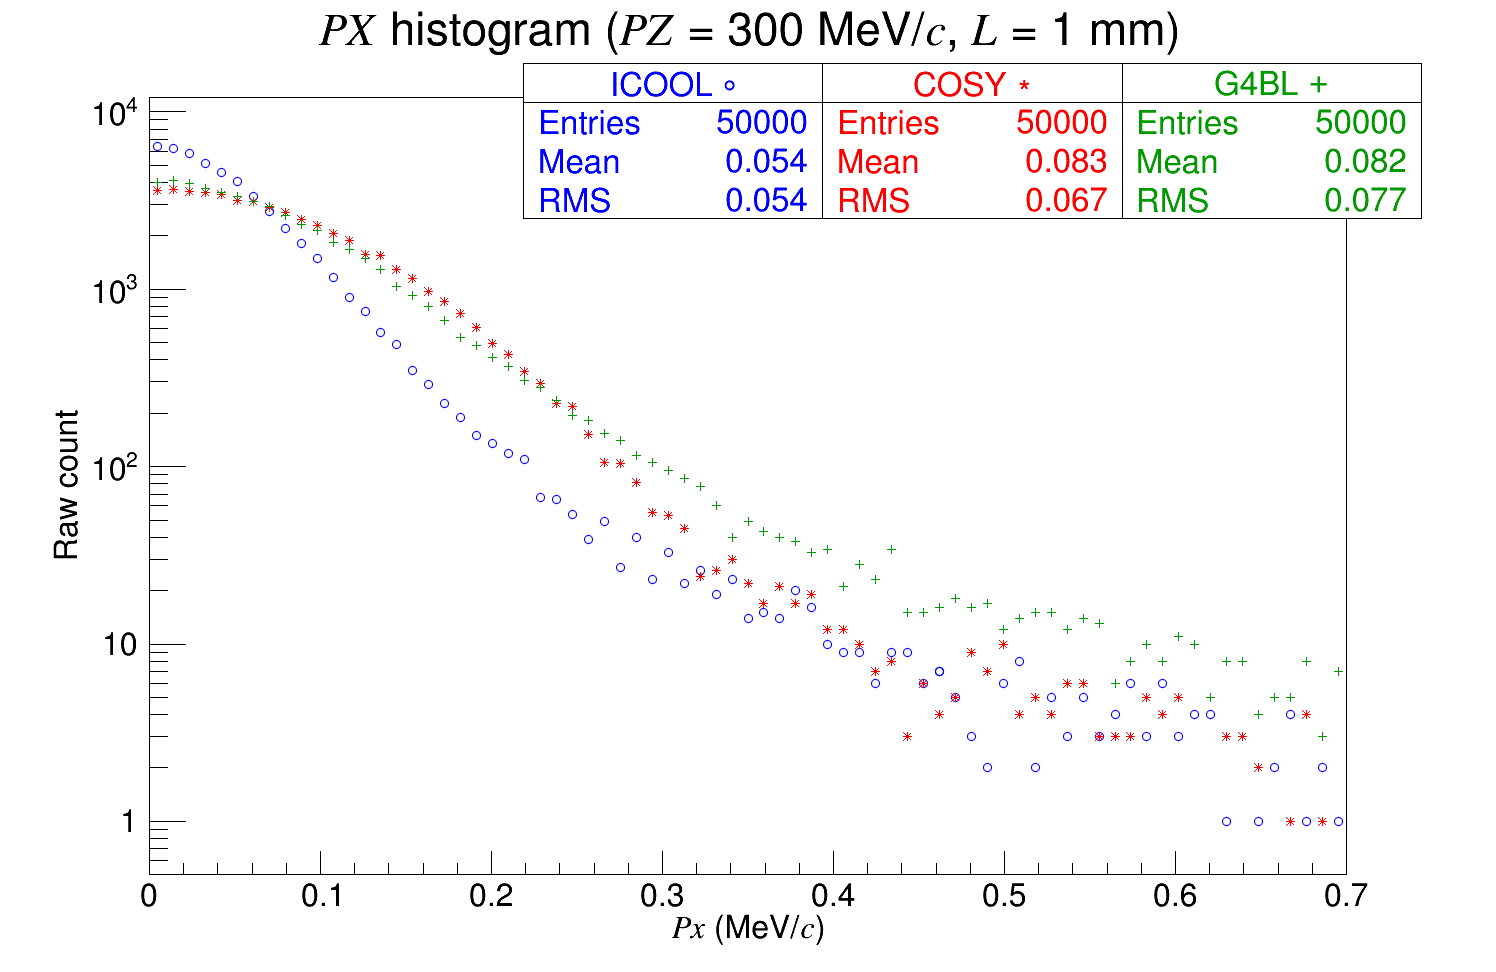
\includegraphics[width=0.7\textwidth]{Benchmarking/LH/PX.300.1.png} 
    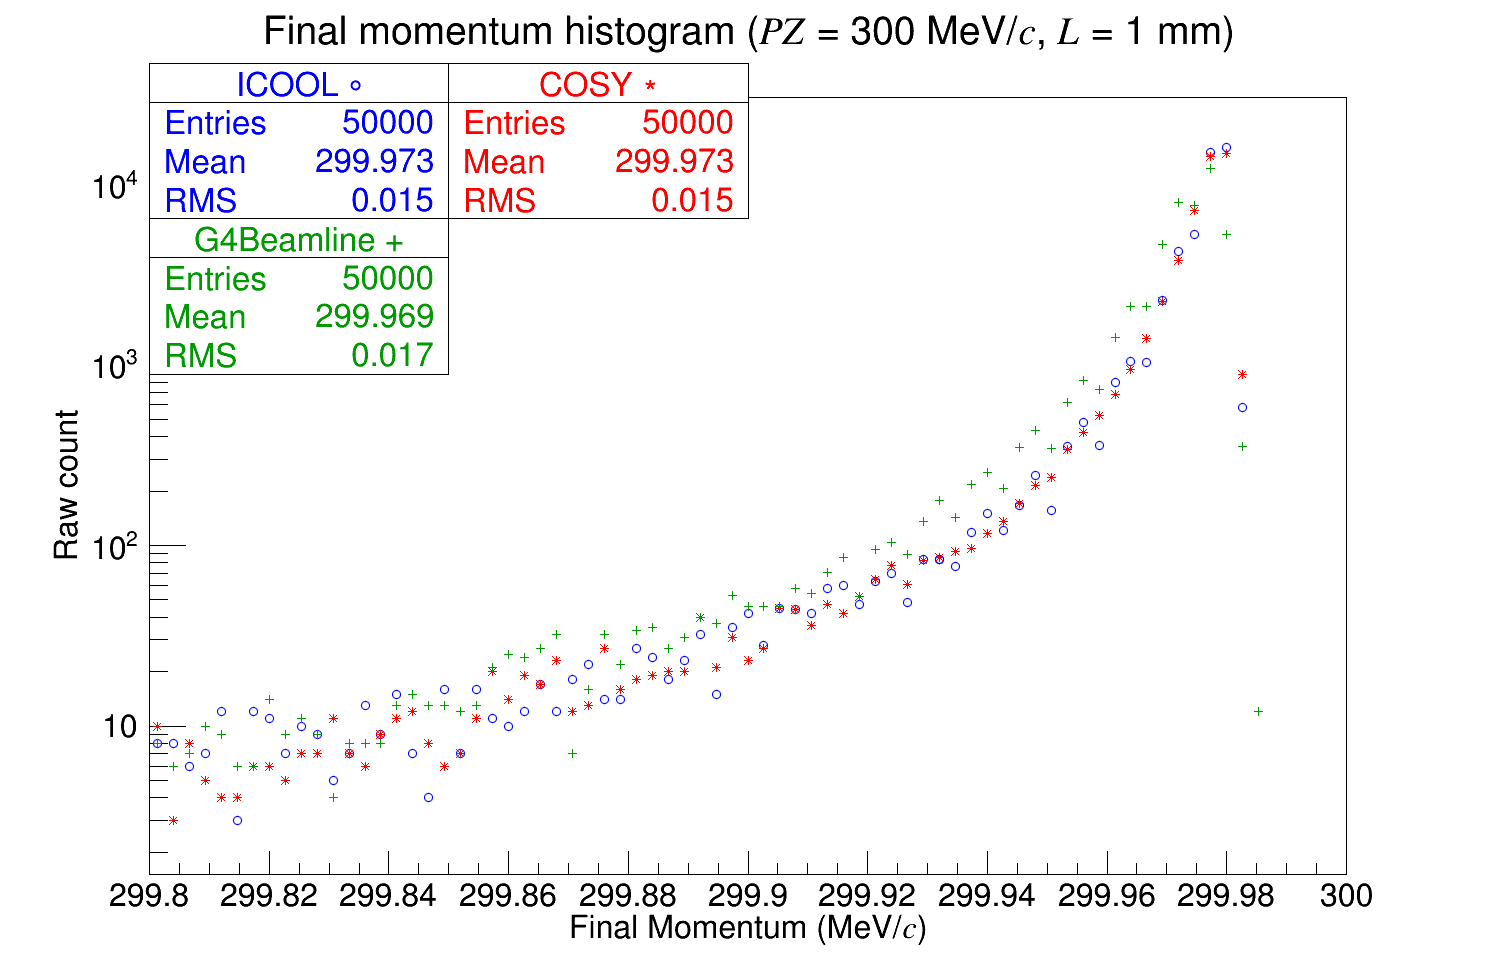
\includegraphics[width=0.7\textwidth]{Benchmarking/LH/strag.300.1.png} 
  \caption[Muons of momentum 300 MeV/$c$ through 1 mm liquid hydrogen.]{Muons of momentum 100 MeV/$c$ through 1 mm liquid hydrogen. Observe that for the $x$ and $p_x$ histograms, COSY and G4Beamline follow a Gaussian-like peak whereas ICOOL follows a Fano peak.}
  \label{fig:300.1}
\end{figure}


\begin{figure}[H]
  \centering
    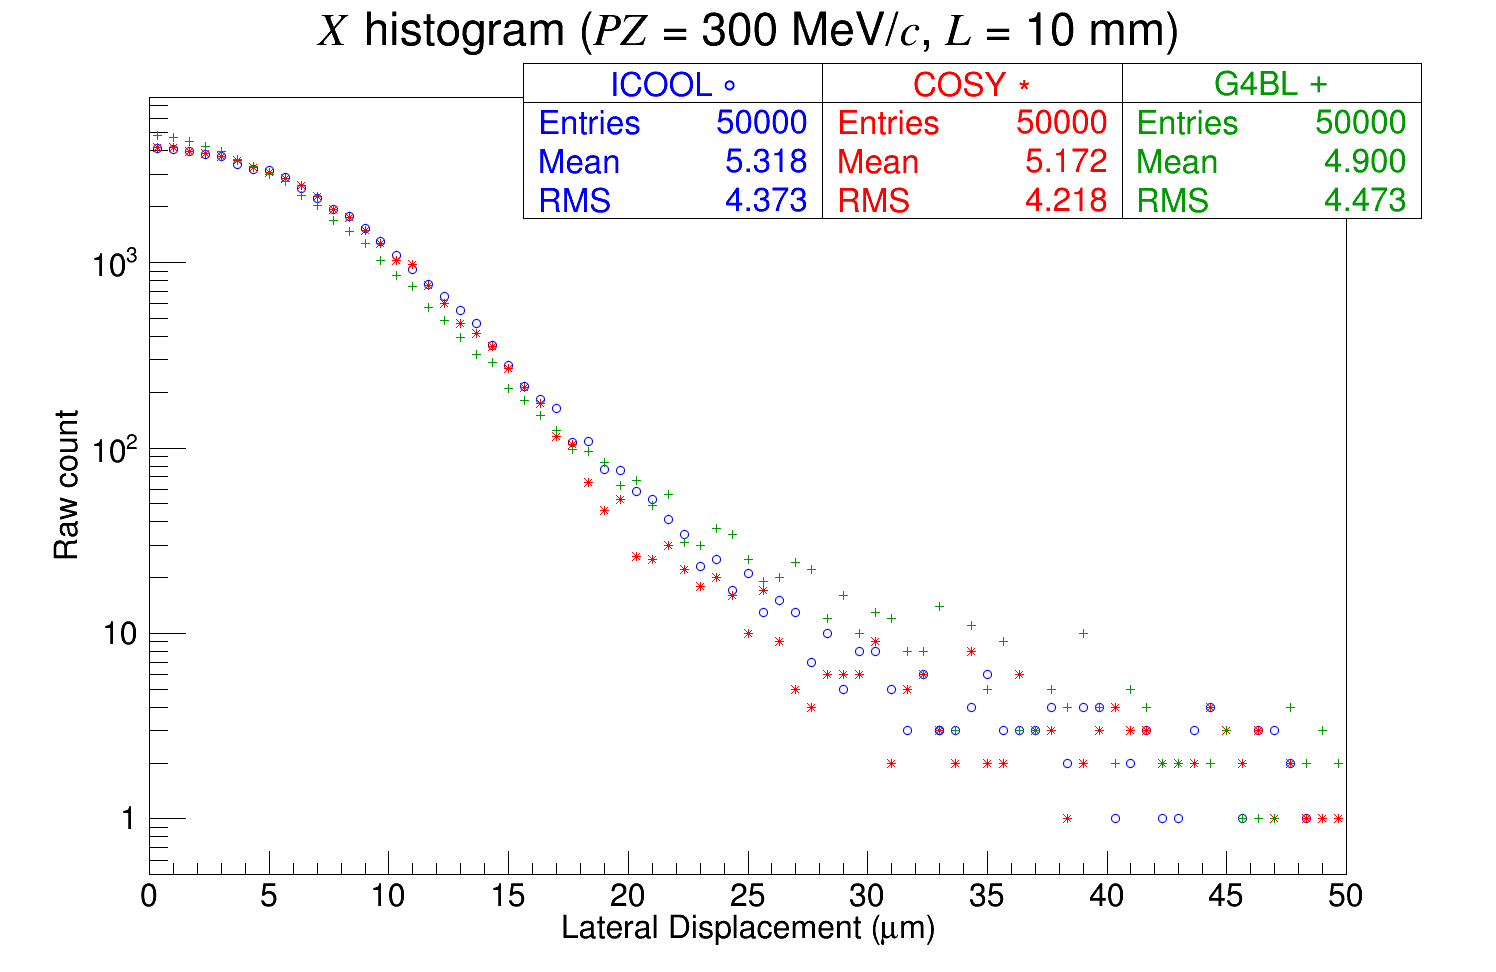
\includegraphics[width=0.7\textwidth]{Benchmarking/LH/X.300.10.png} 
    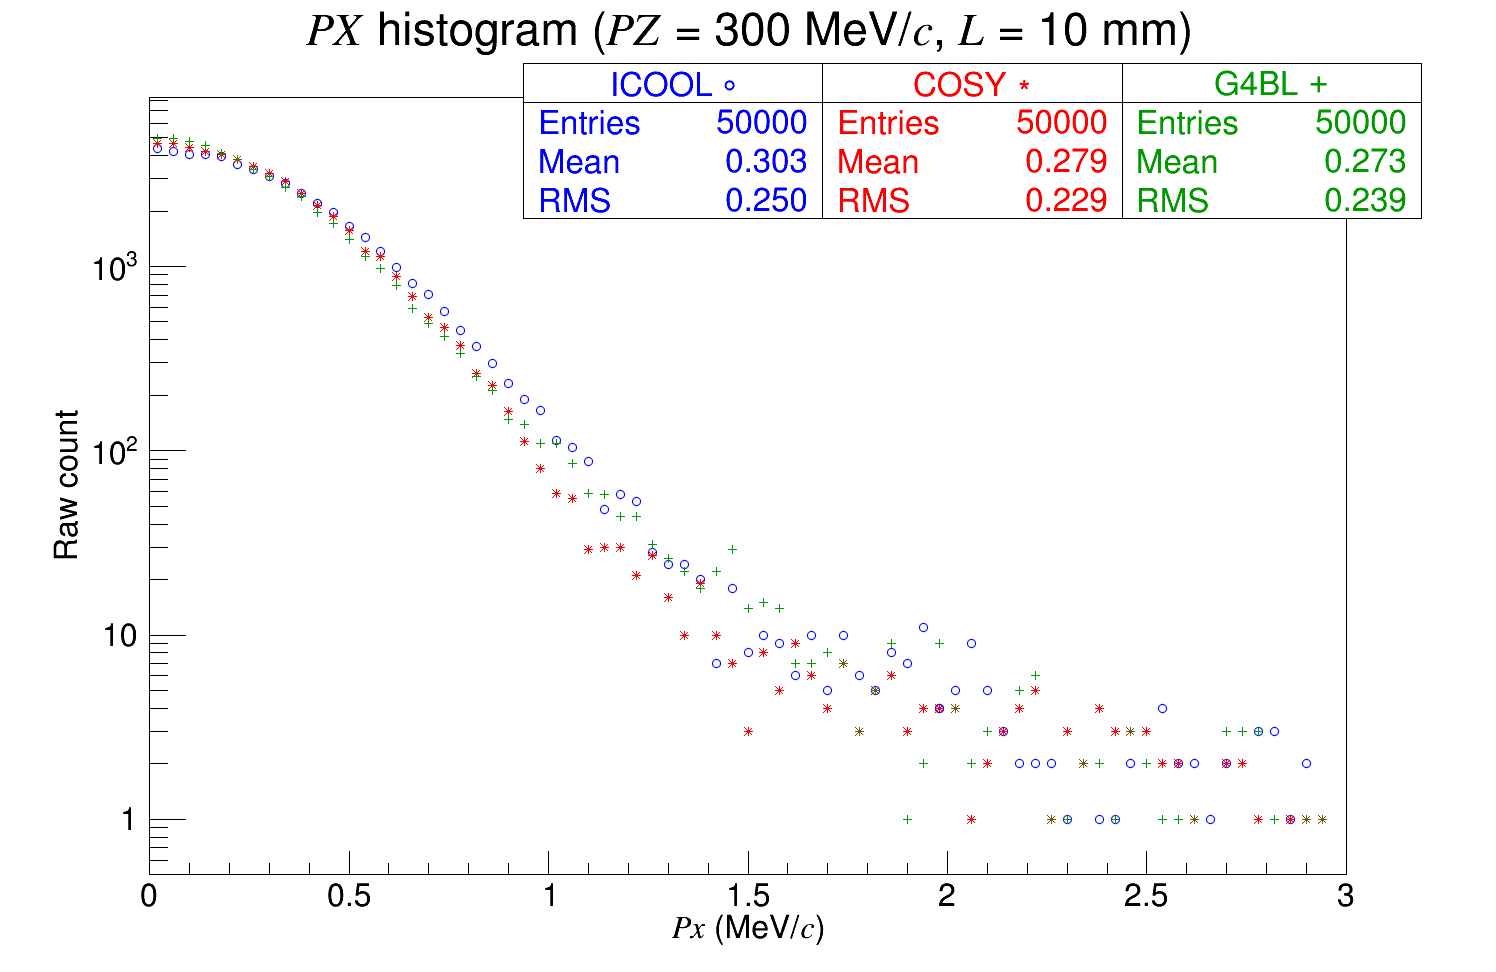
\includegraphics[width=0.7\textwidth]{Benchmarking/LH/PX.300.10.png} 
    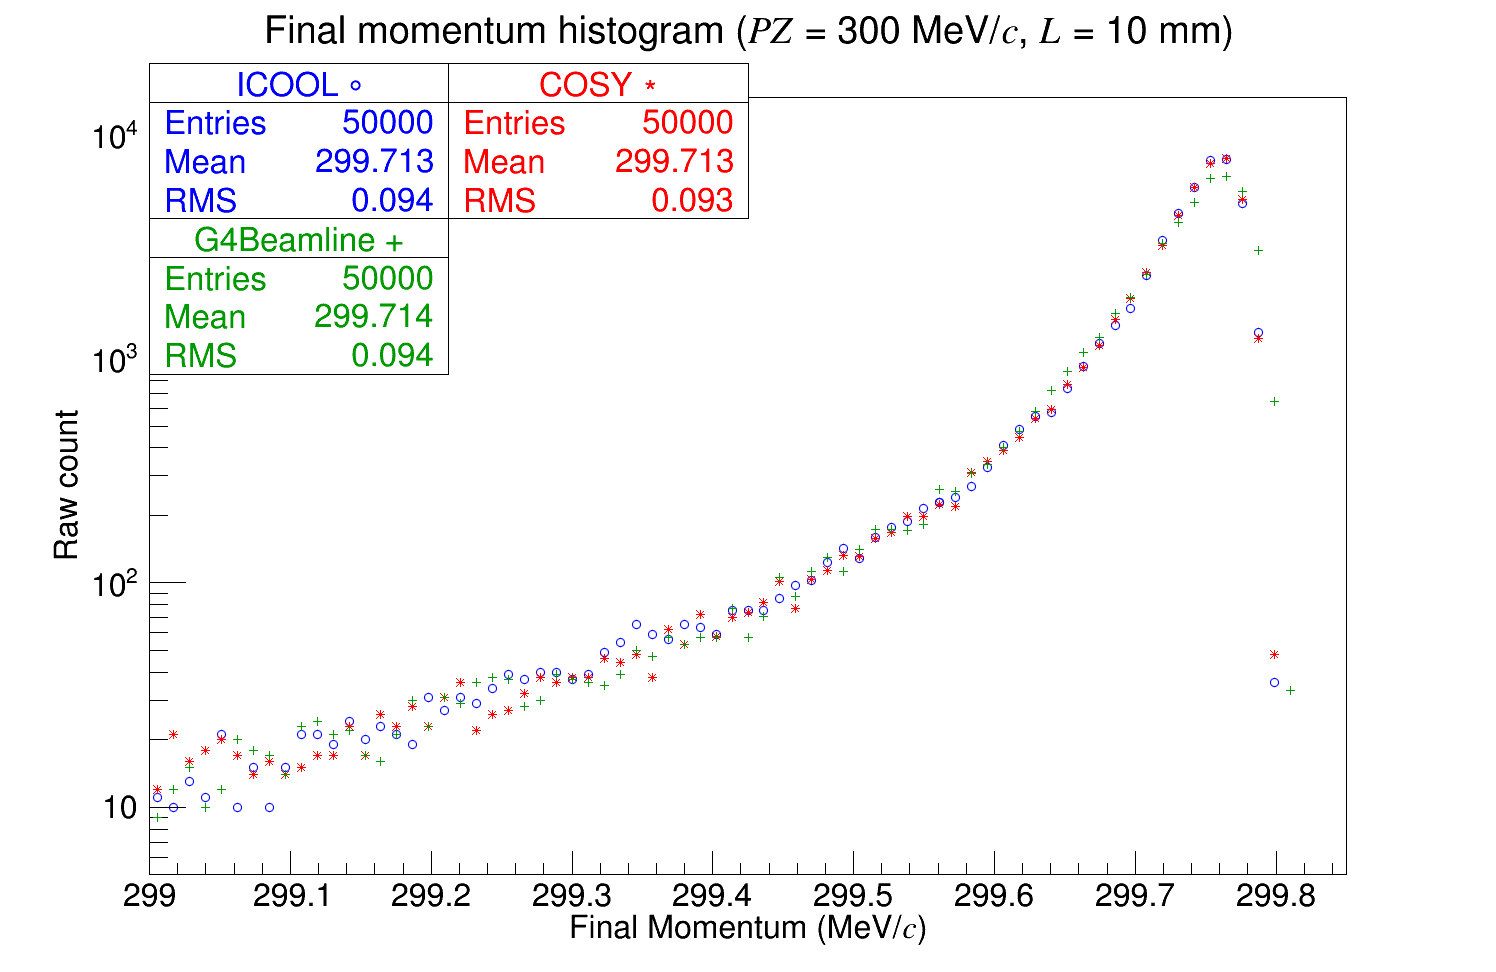
\includegraphics[width=0.7\textwidth]{Benchmarking/LH/strag.300.10.png} 
  \caption{Muons of momentum 300 MeV/$c$ through 10 mm liquid hydrogen.}
  \label{fig:300.10}
\end{figure}

\begin{figure}[!htb]
  \centering
    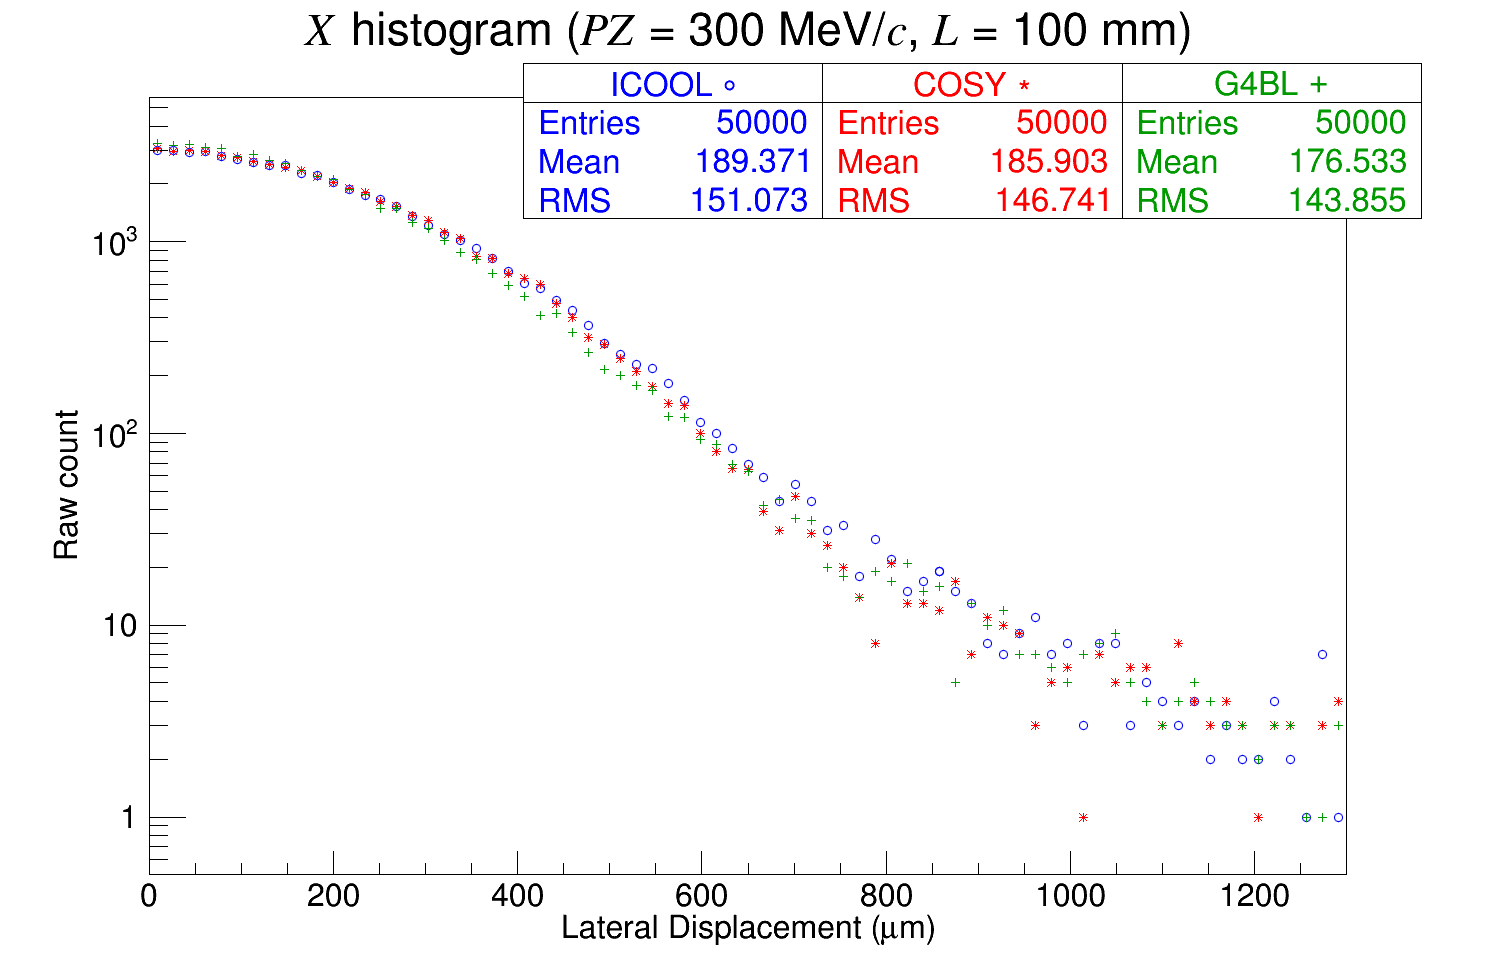
\includegraphics[width=0.7\textwidth]{Benchmarking/LH/X.300.100.png} 
    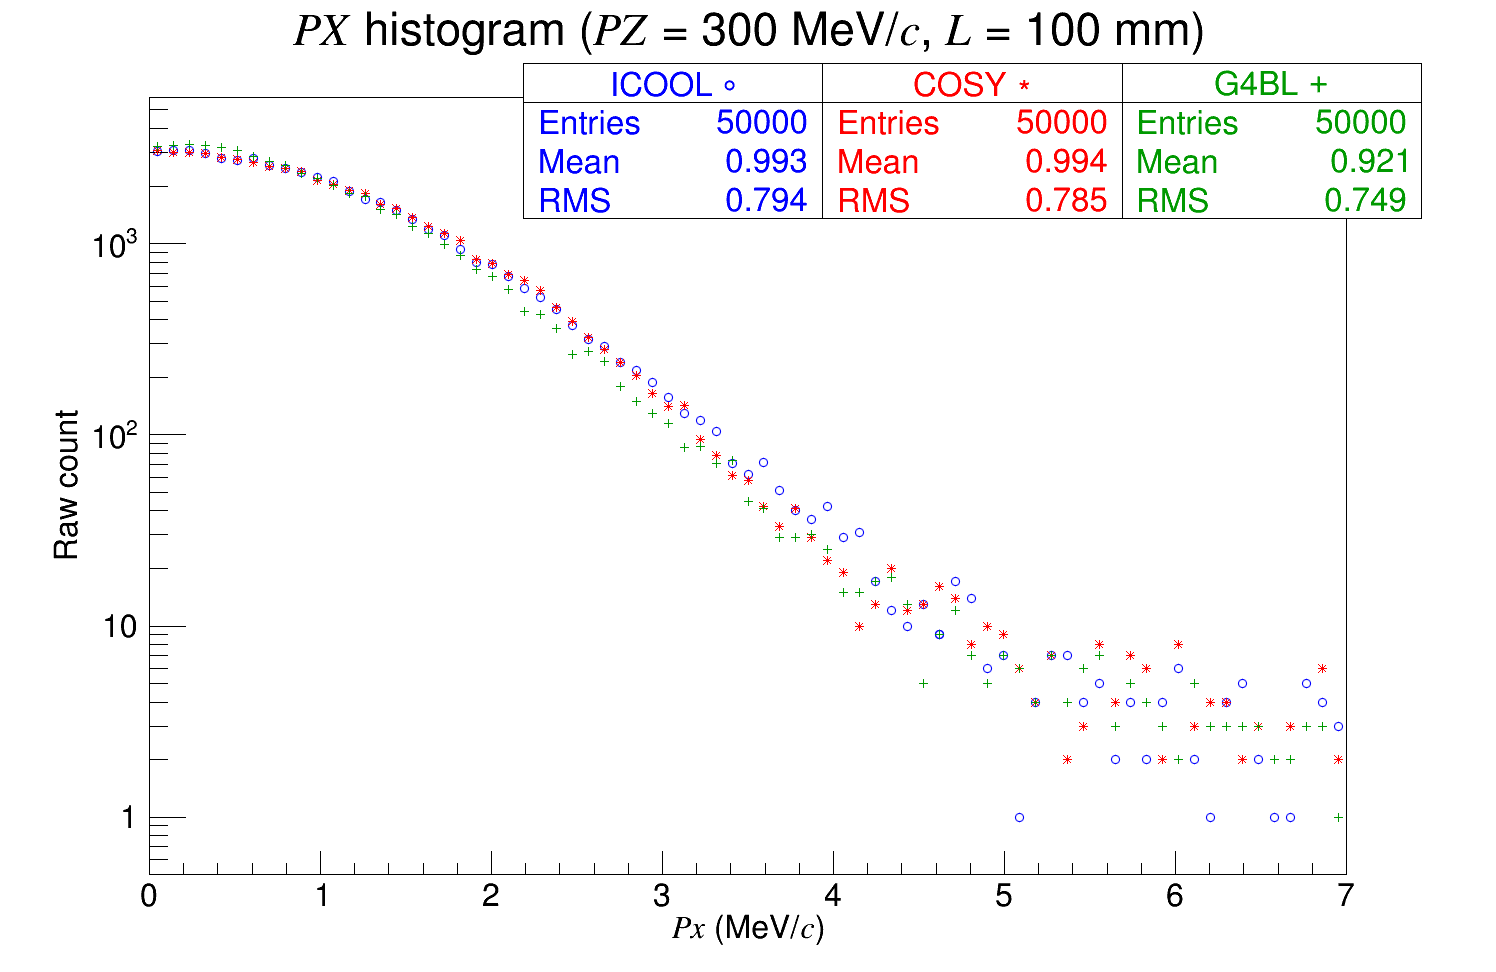
\includegraphics[width=0.7\textwidth]{Benchmarking/LH/PX.300.100.png} 
    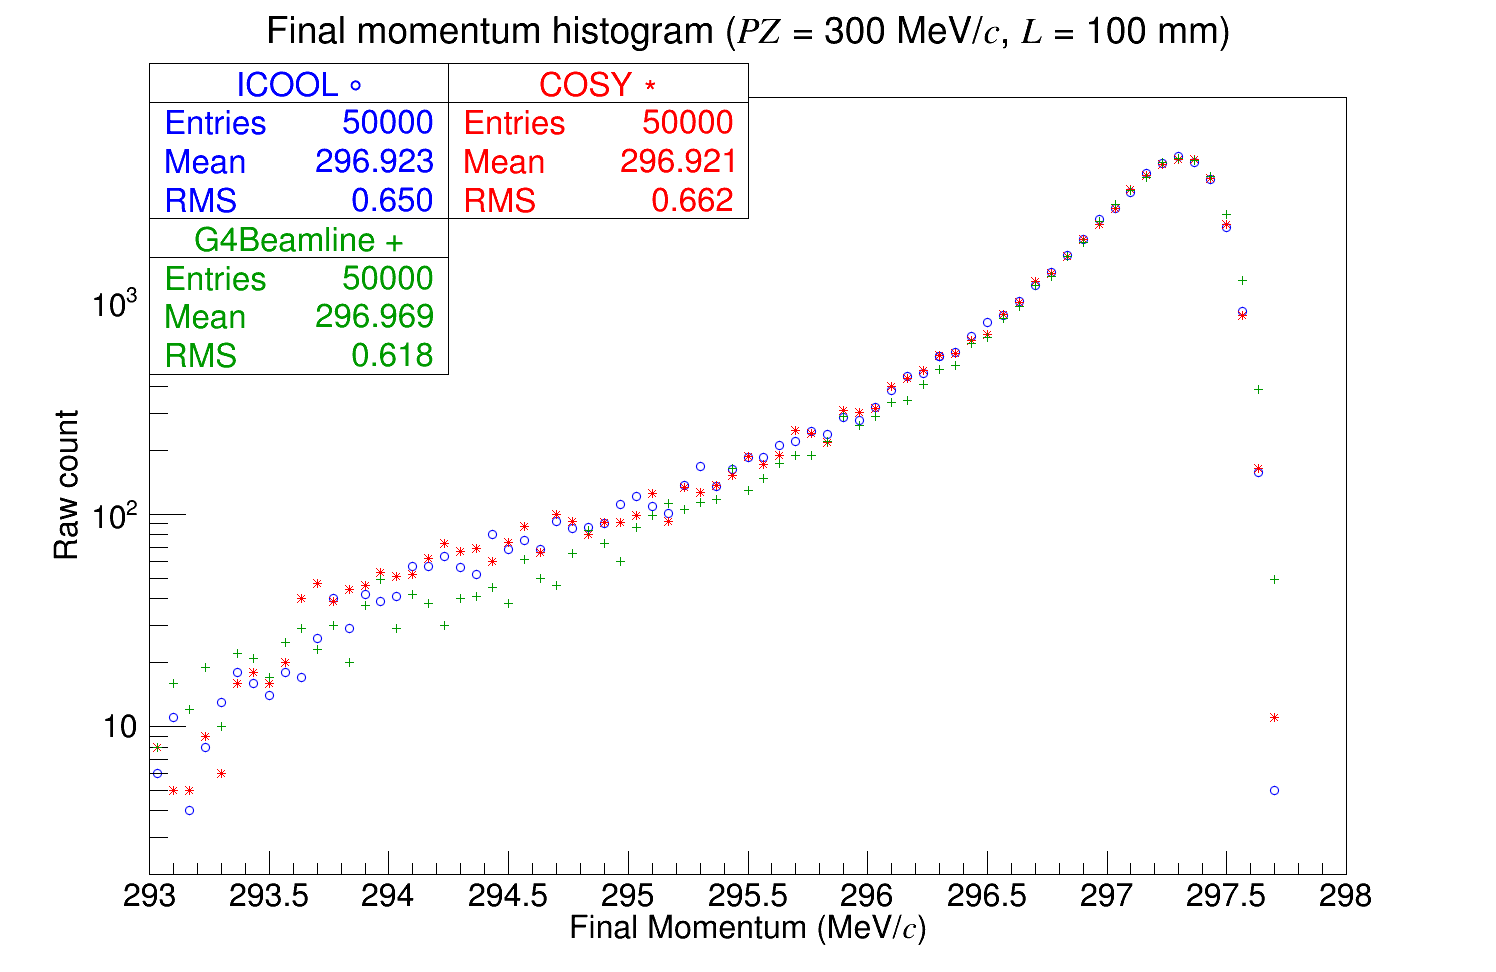
\includegraphics[width=0.7\textwidth]{Benchmarking/LH/strag.300.100.png} 
  \caption{Muons of momentum 300 MeV/$c$ through 100 mm liquid hydrogen.}
  \label{fig:300.100}
\end{figure}

\begin{figure}[H]
  \centering
    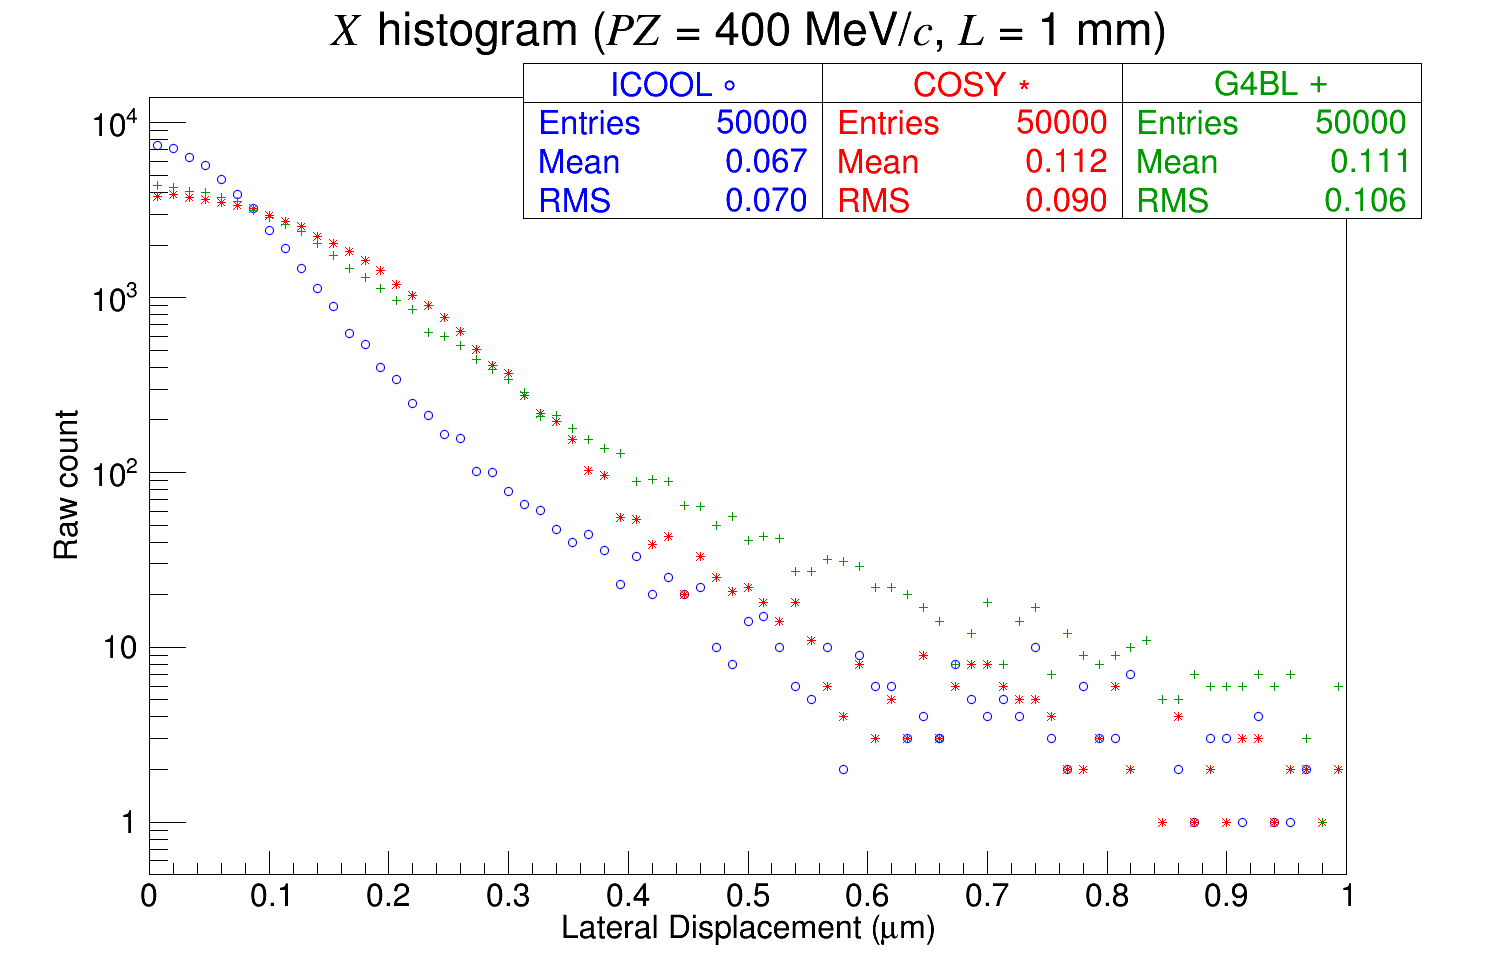
\includegraphics[width=0.7\textwidth]{Benchmarking/LH/X.400.1.png} 
    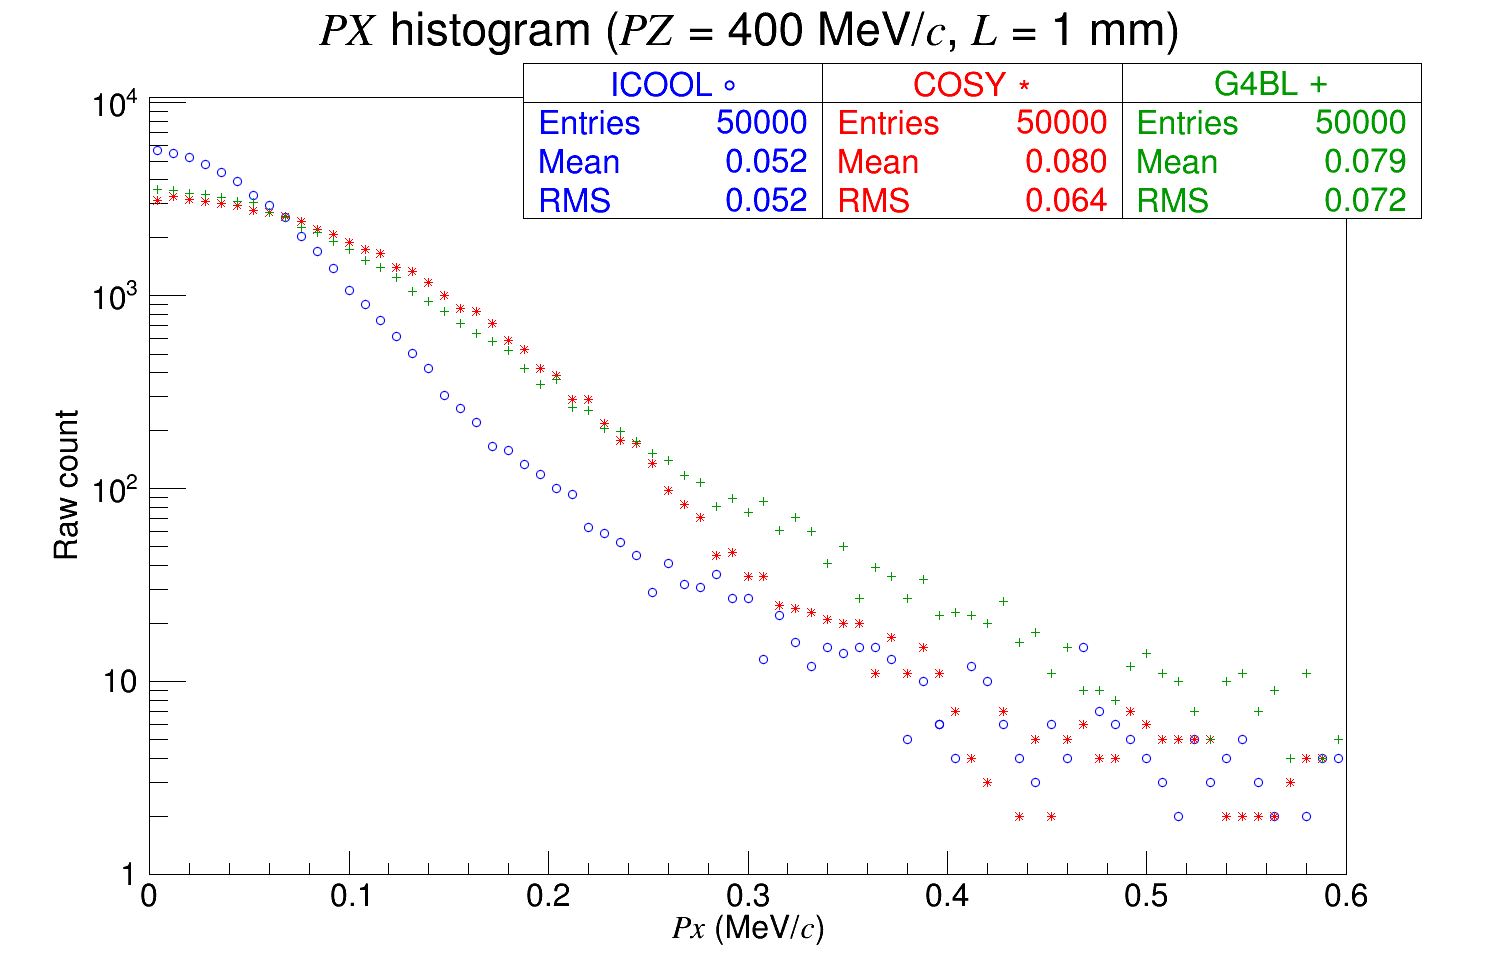
\includegraphics[width=0.7\textwidth]{Benchmarking/LH/PX.400.1.png} 
    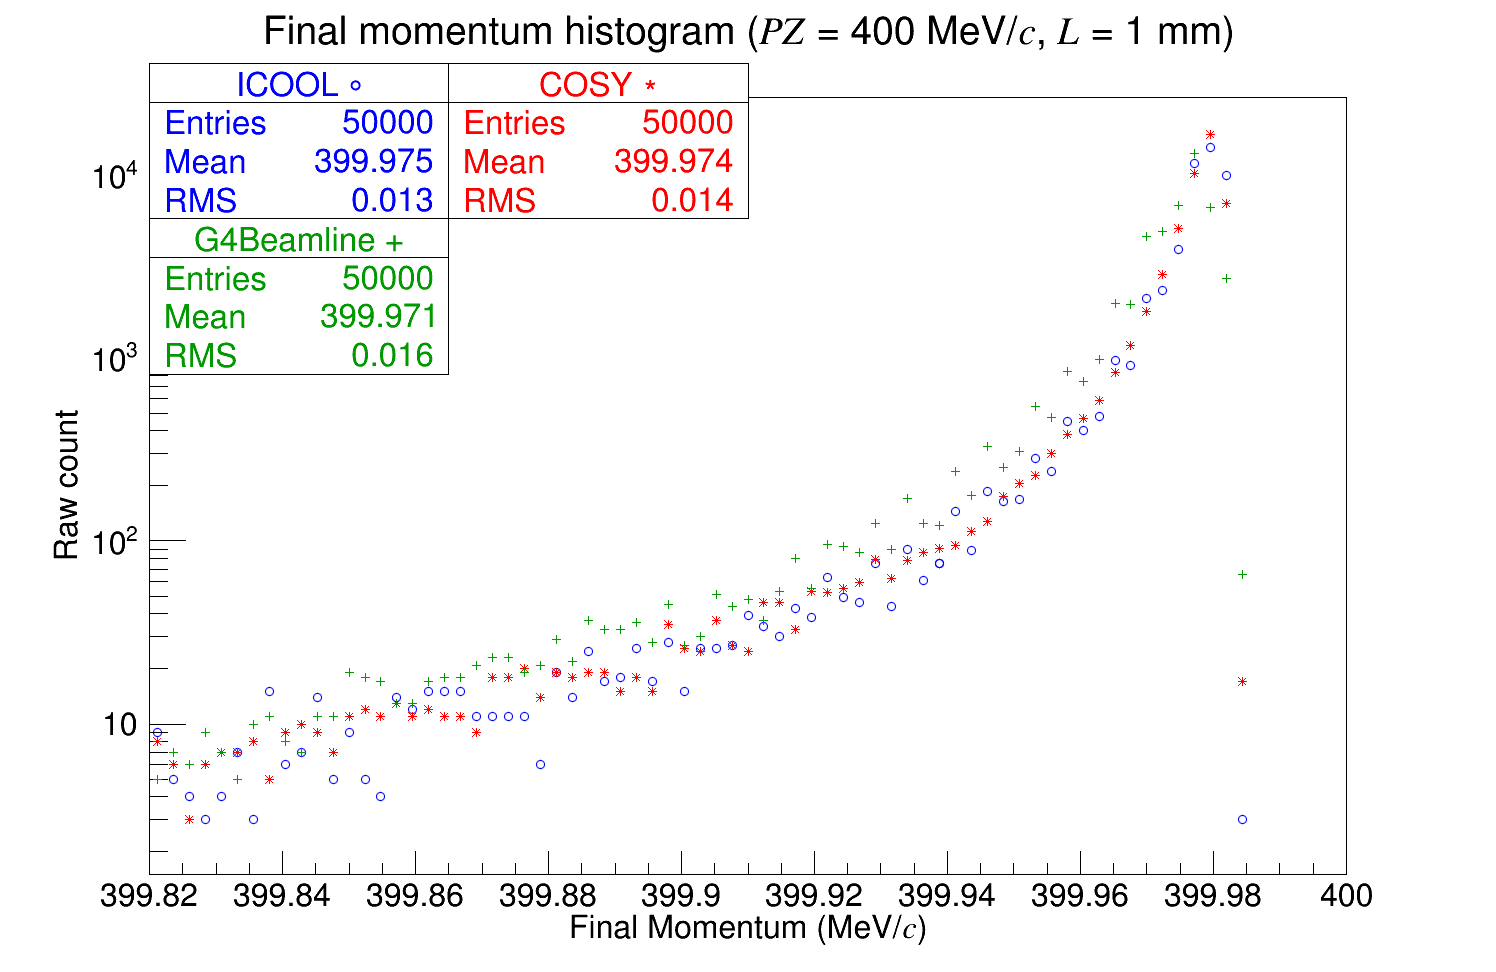
\includegraphics[width=0.7\textwidth]{Benchmarking/LH/strag.400.1.png} 
  \caption[Muons of momentum 400 MeV/$c$ through 1 mm liquid hydrogen.]{Muons of momentum 100 MeV/$c$ through 1 mm liquid hydrogen. Observe that for the $x$ and $p_x$ histograms, COSY and G4Beamline follow a Gaussian-like peak whereas ICOOL follows a Fano peak.}
  \label{fig:400.1}
\end{figure}

\begin{figure}[H]
  \centering
    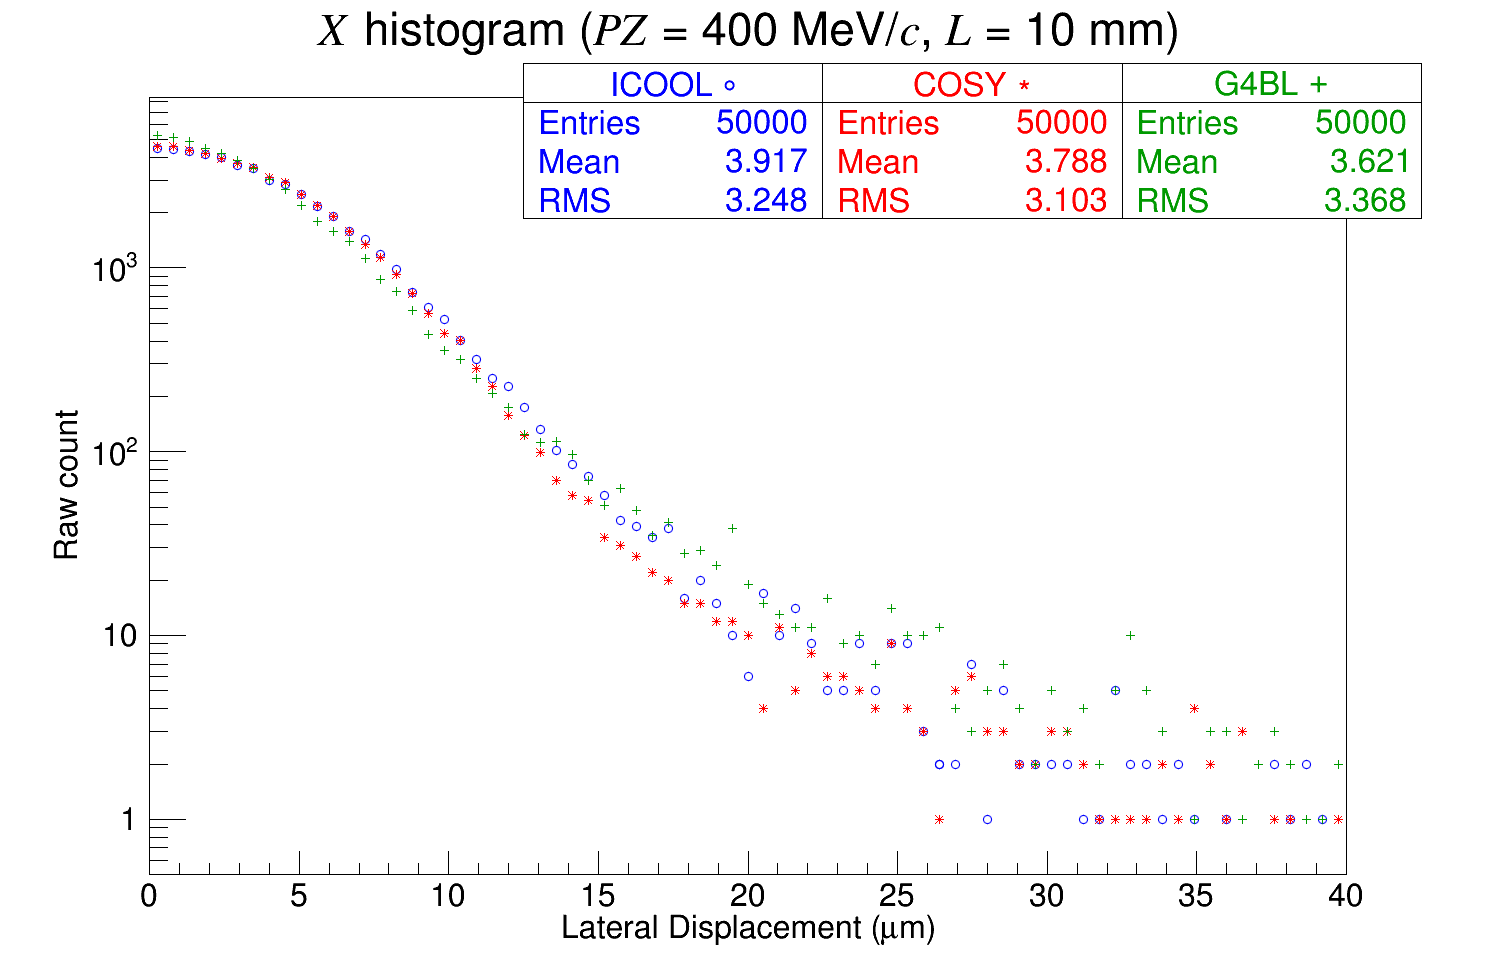
\includegraphics[width=0.7\textwidth]{Benchmarking/LH/X.400.10.png} 
    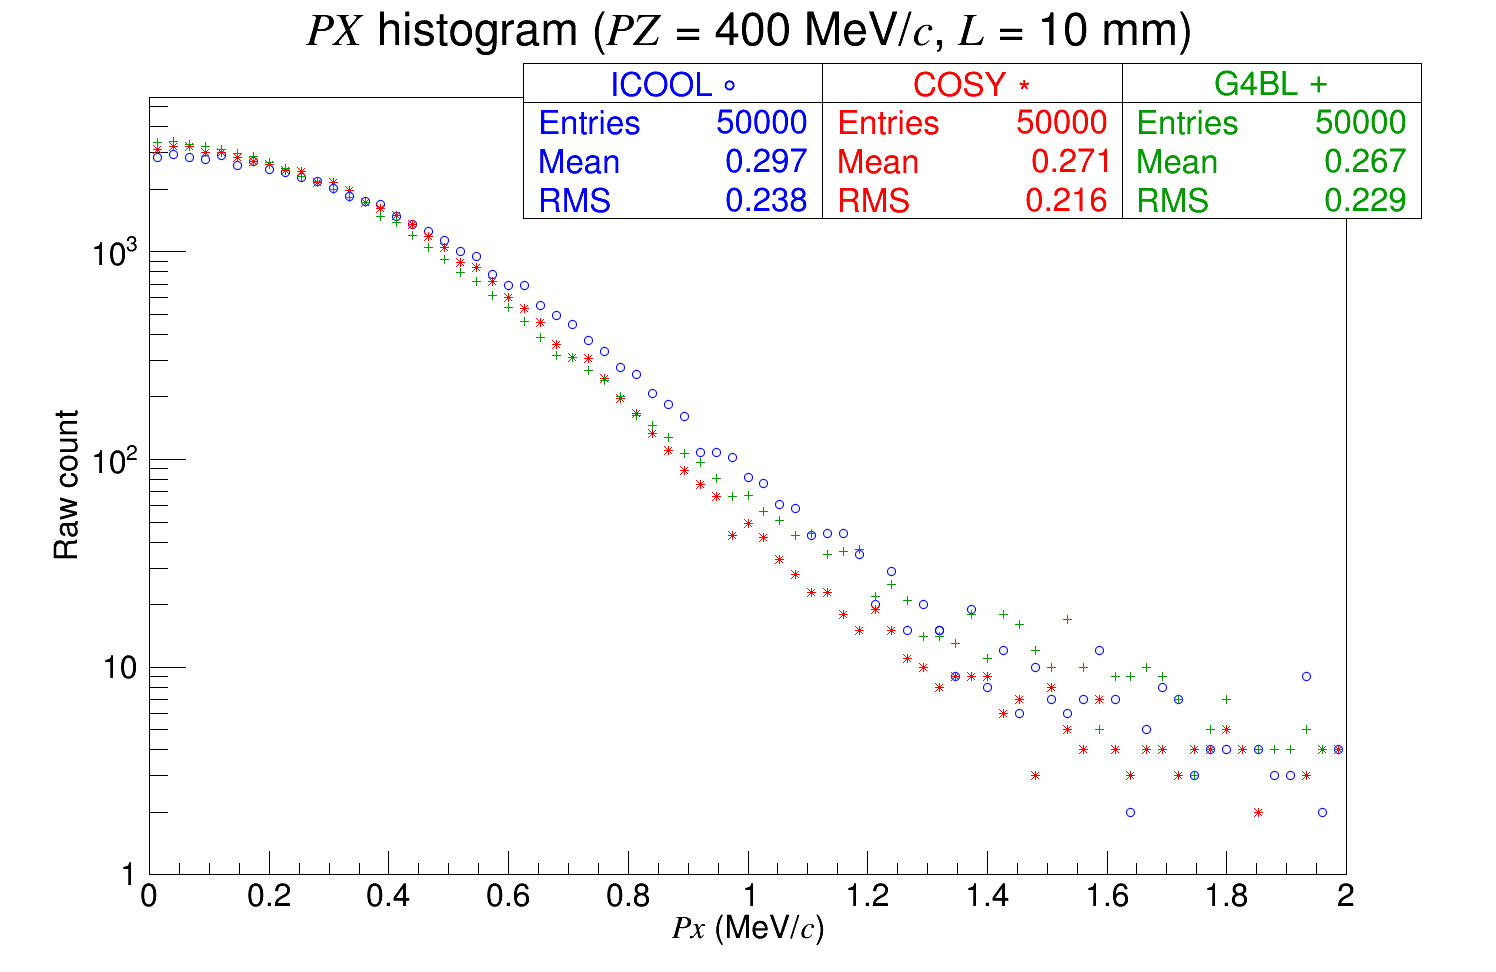
\includegraphics[width=0.7\textwidth]{Benchmarking/LH/PX.400.10.png} 
    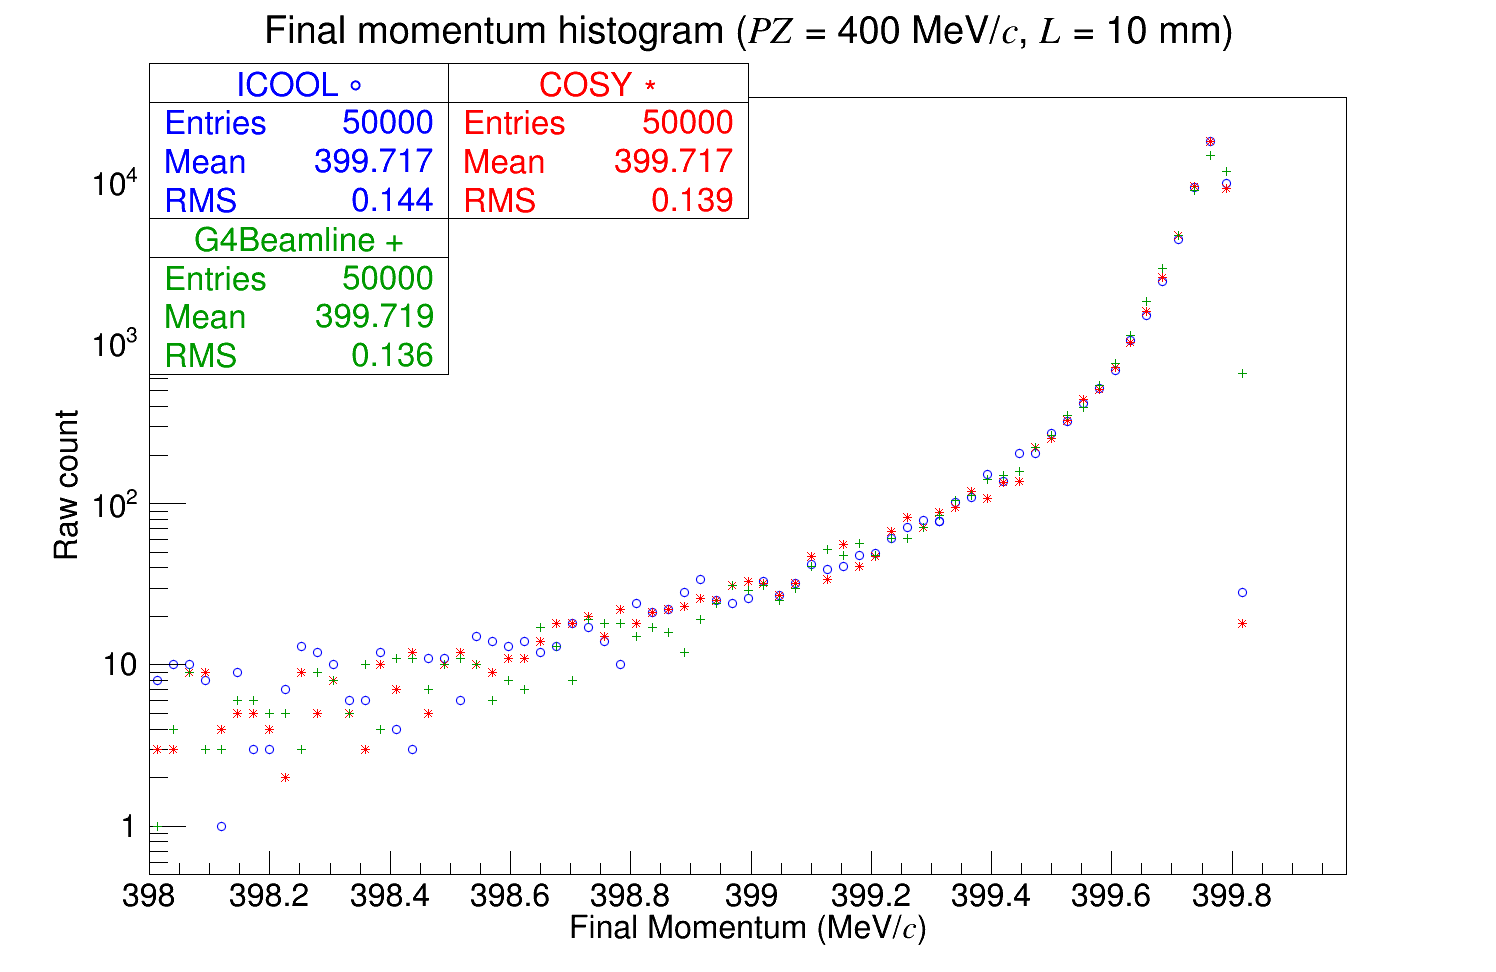
\includegraphics[width=0.7\textwidth]{Benchmarking/LH/strag.400.10.png} 
  \caption{Muons of momentum 400 MeV/$c$ through 10 mm liquid hydrogen.}
  \label{fig:400.10}
\end{figure}

\begin{figure}[H]
  \centering
    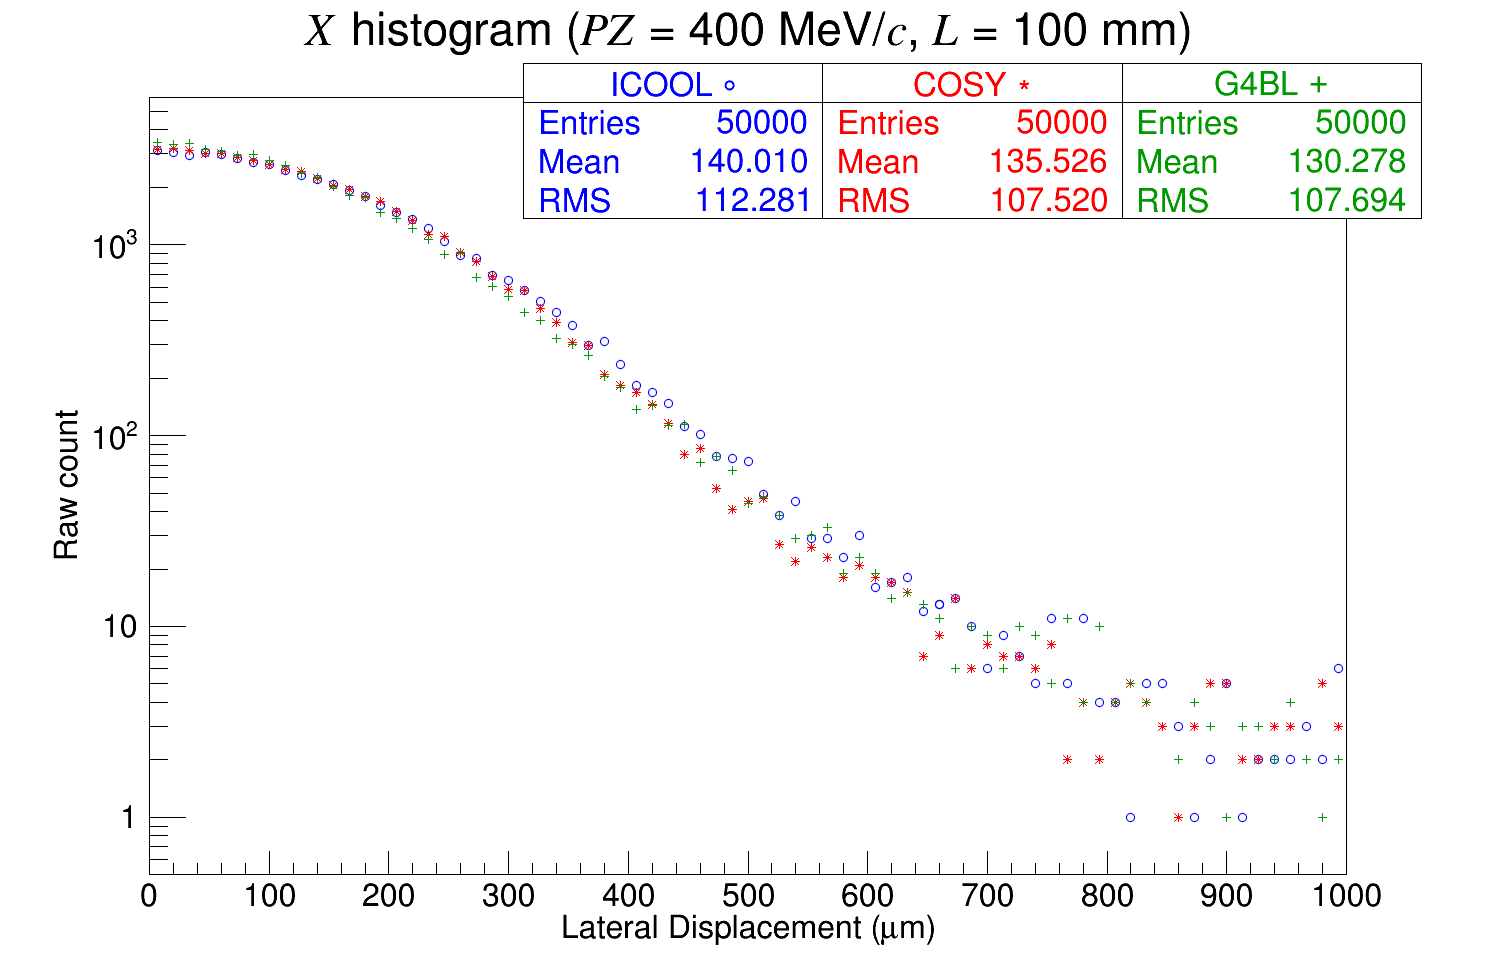
\includegraphics[width=0.7\textwidth]{Benchmarking/LH/X.400.100.png} 
    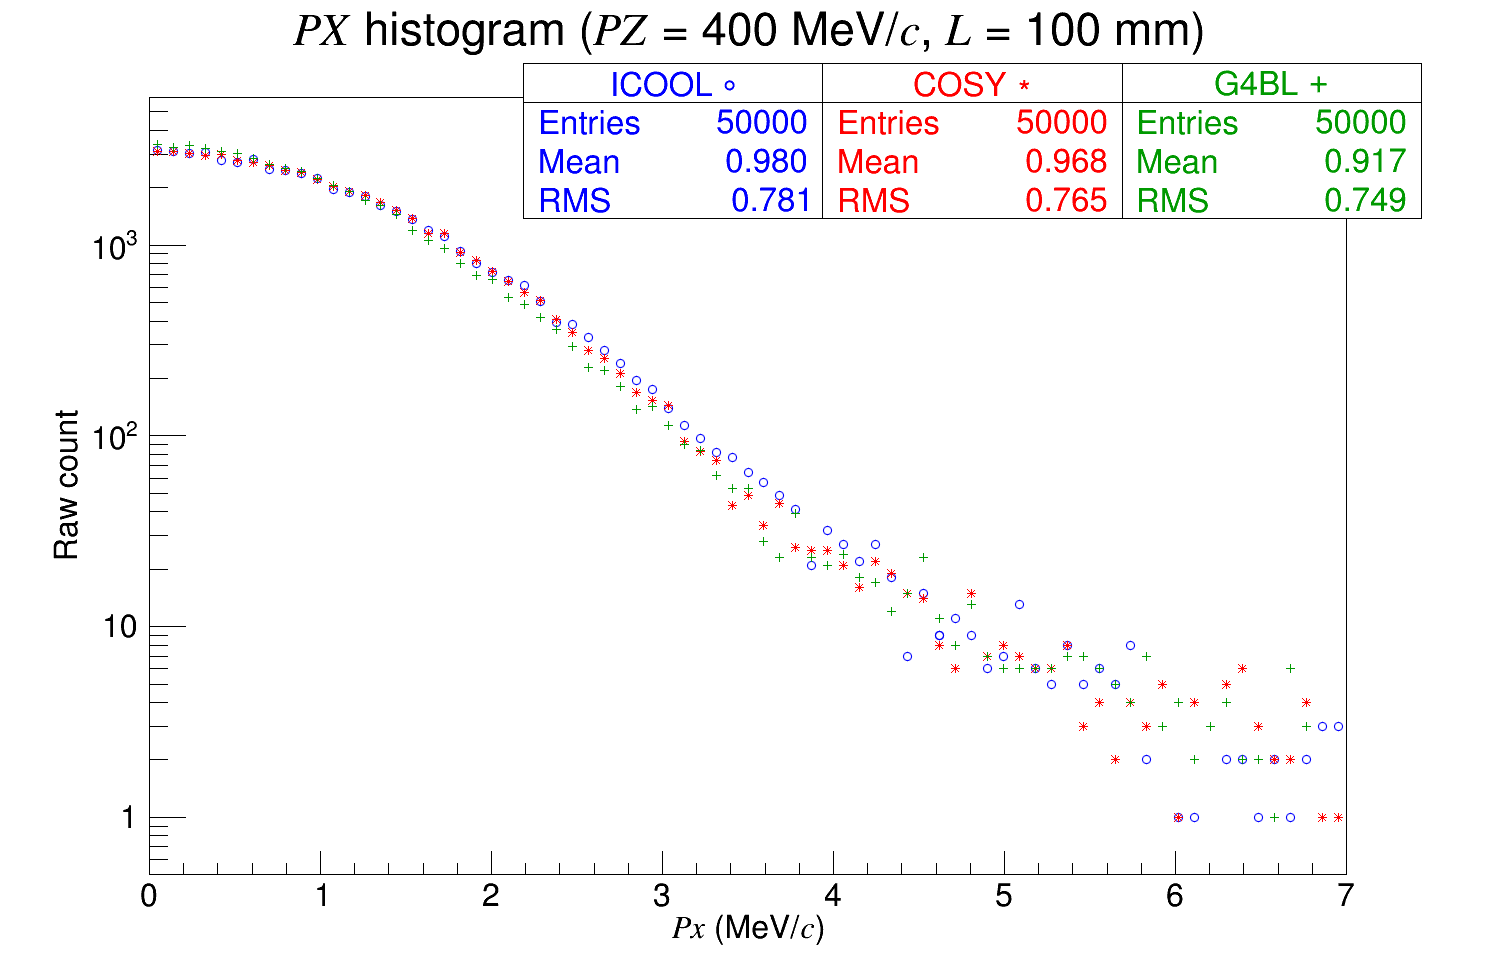
\includegraphics[width=0.7\textwidth]{Benchmarking/LH/PX.400.100.png} 
    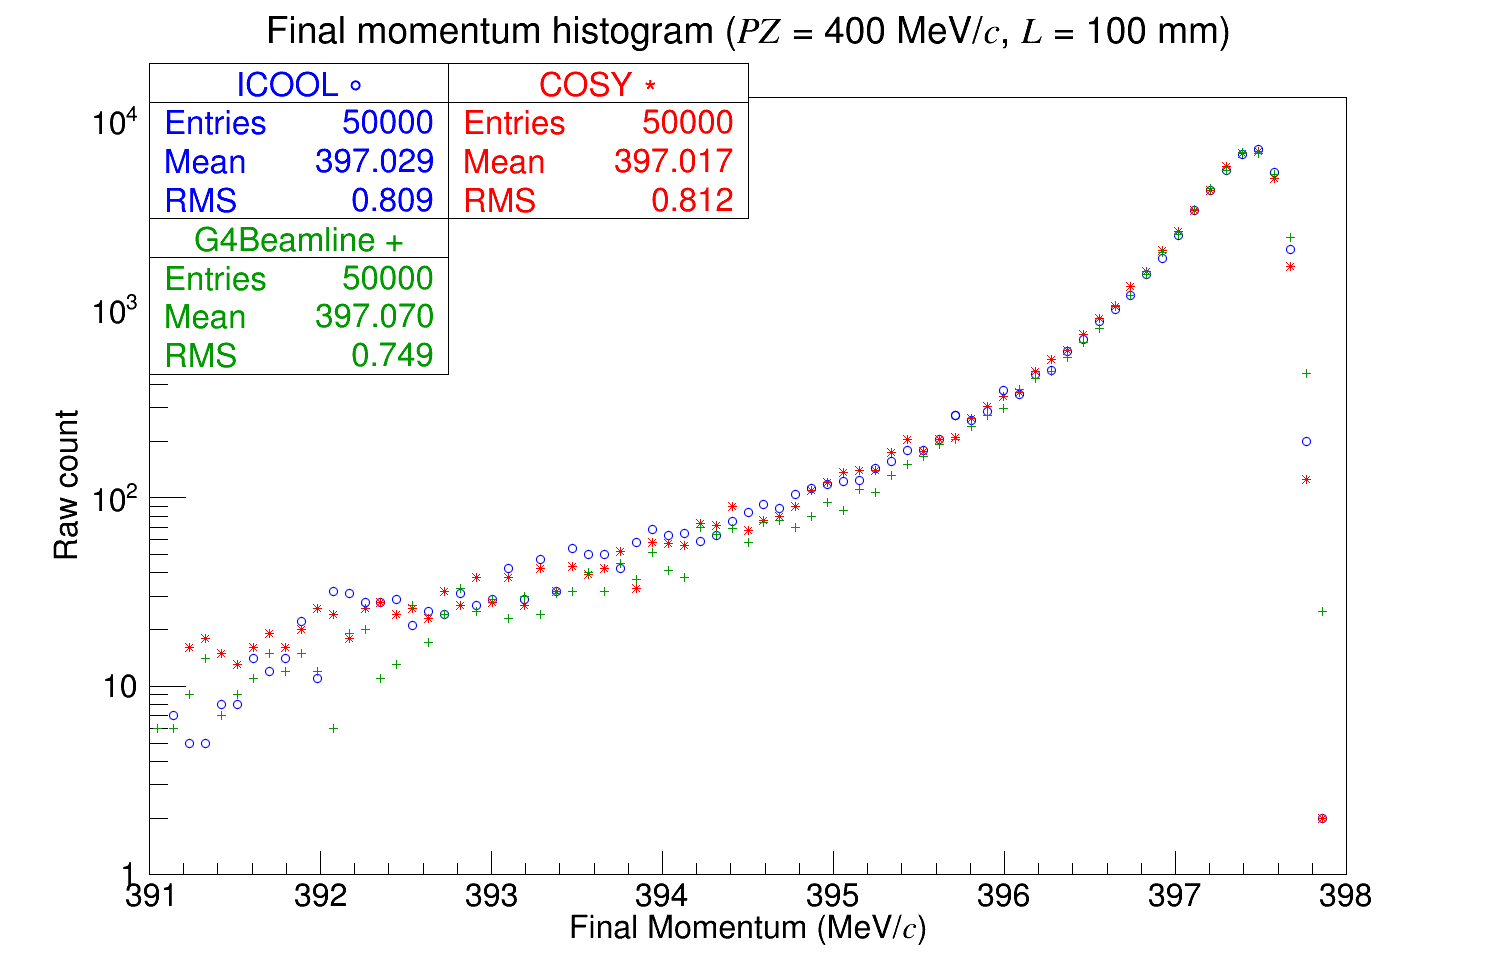
\includegraphics[width=0.7\textwidth]{Benchmarking/LH/strag.400.100.png} 
  \caption{Muons of momentum 400 MeV/$c$ through 100 mm liquid hydrogen.}
  \label{fig:400.100}
\end{figure}


For the 1 mm figures (Figures \ref{fig:100.1}, \ref{fig:200.1}, \ref{fig:300.1}, and \ref{fig:400.1}) there is much disagreement between the codes' transverse momentum distributions. Since the transverse momentum and transverse position coordinates are related, there is also disagreement among the transverse position distributions. This is likely because the default ICOOL scattering model uses a Fano peak with a Rutherford tail whereas both COSY and G4Beamline use a Gaussian peak. It can be seen by, e.g., Figure~\ref{fig:100.1} that COSY, like G4Beamline, uses the Gaussian model for the peak but, like ICOOL, then switches to a Rutherford tail.

For the 10 mm figures (Figures \ref{fig:100.10}, \ref{fig:200.10}, \ref{fig:300.10}, and \ref{fig:400.10}), both $x$ and $p_x$ distributions agree well. For COSY, the tail of the distribution falls off slightly faster after approximately 1~MeV/$c$. 

For the final momentum plots, ICOOL and COSY agree quite well. This is not surprising since both codes use Landau theory to describe the energy loss distribution. G4Beamline occasionally disagrees. An example of this can be seen in Figure~\ref{fig:200.1}. However, given the scale of the horizontal axis this disagreement is much smaller than it initially appears.

\Section{Validation}\label{sec:validation}

The new COSY routines were also compared to the Muon Scattering Experiment \cite{muscat}, often referred to as MuScat. This experiment measured the scattering of a beam of collimated muons through seven materials. To emulate this, pencil beams with momentum $P=172$ MeV/$c$ were created in COSY, G4Beamline, and ICOOL. The pencil beam consisted of $5\times10^6$ particles and was propagated through 109 mm of liquid hydrogen, 159 mm of liquid hydrogen, and 3.73 mm of beryllium. Liquid hydrogen was chosen to represent muons through long absorbers of low-$Z$ materials. Beryllium, on the other hand, was chosen to represent muons through much thinner and denser media. COSY took a single step through the absorbers while G4BL took a step size of 1 mm. The data points were normalized to the total probability, was calculated via Simpson's rule. The probability per radian was then found by dividing the probability of the data point by the scattered angle at that point. The results are shown below.

\begin{figure}[H]
  \centering
    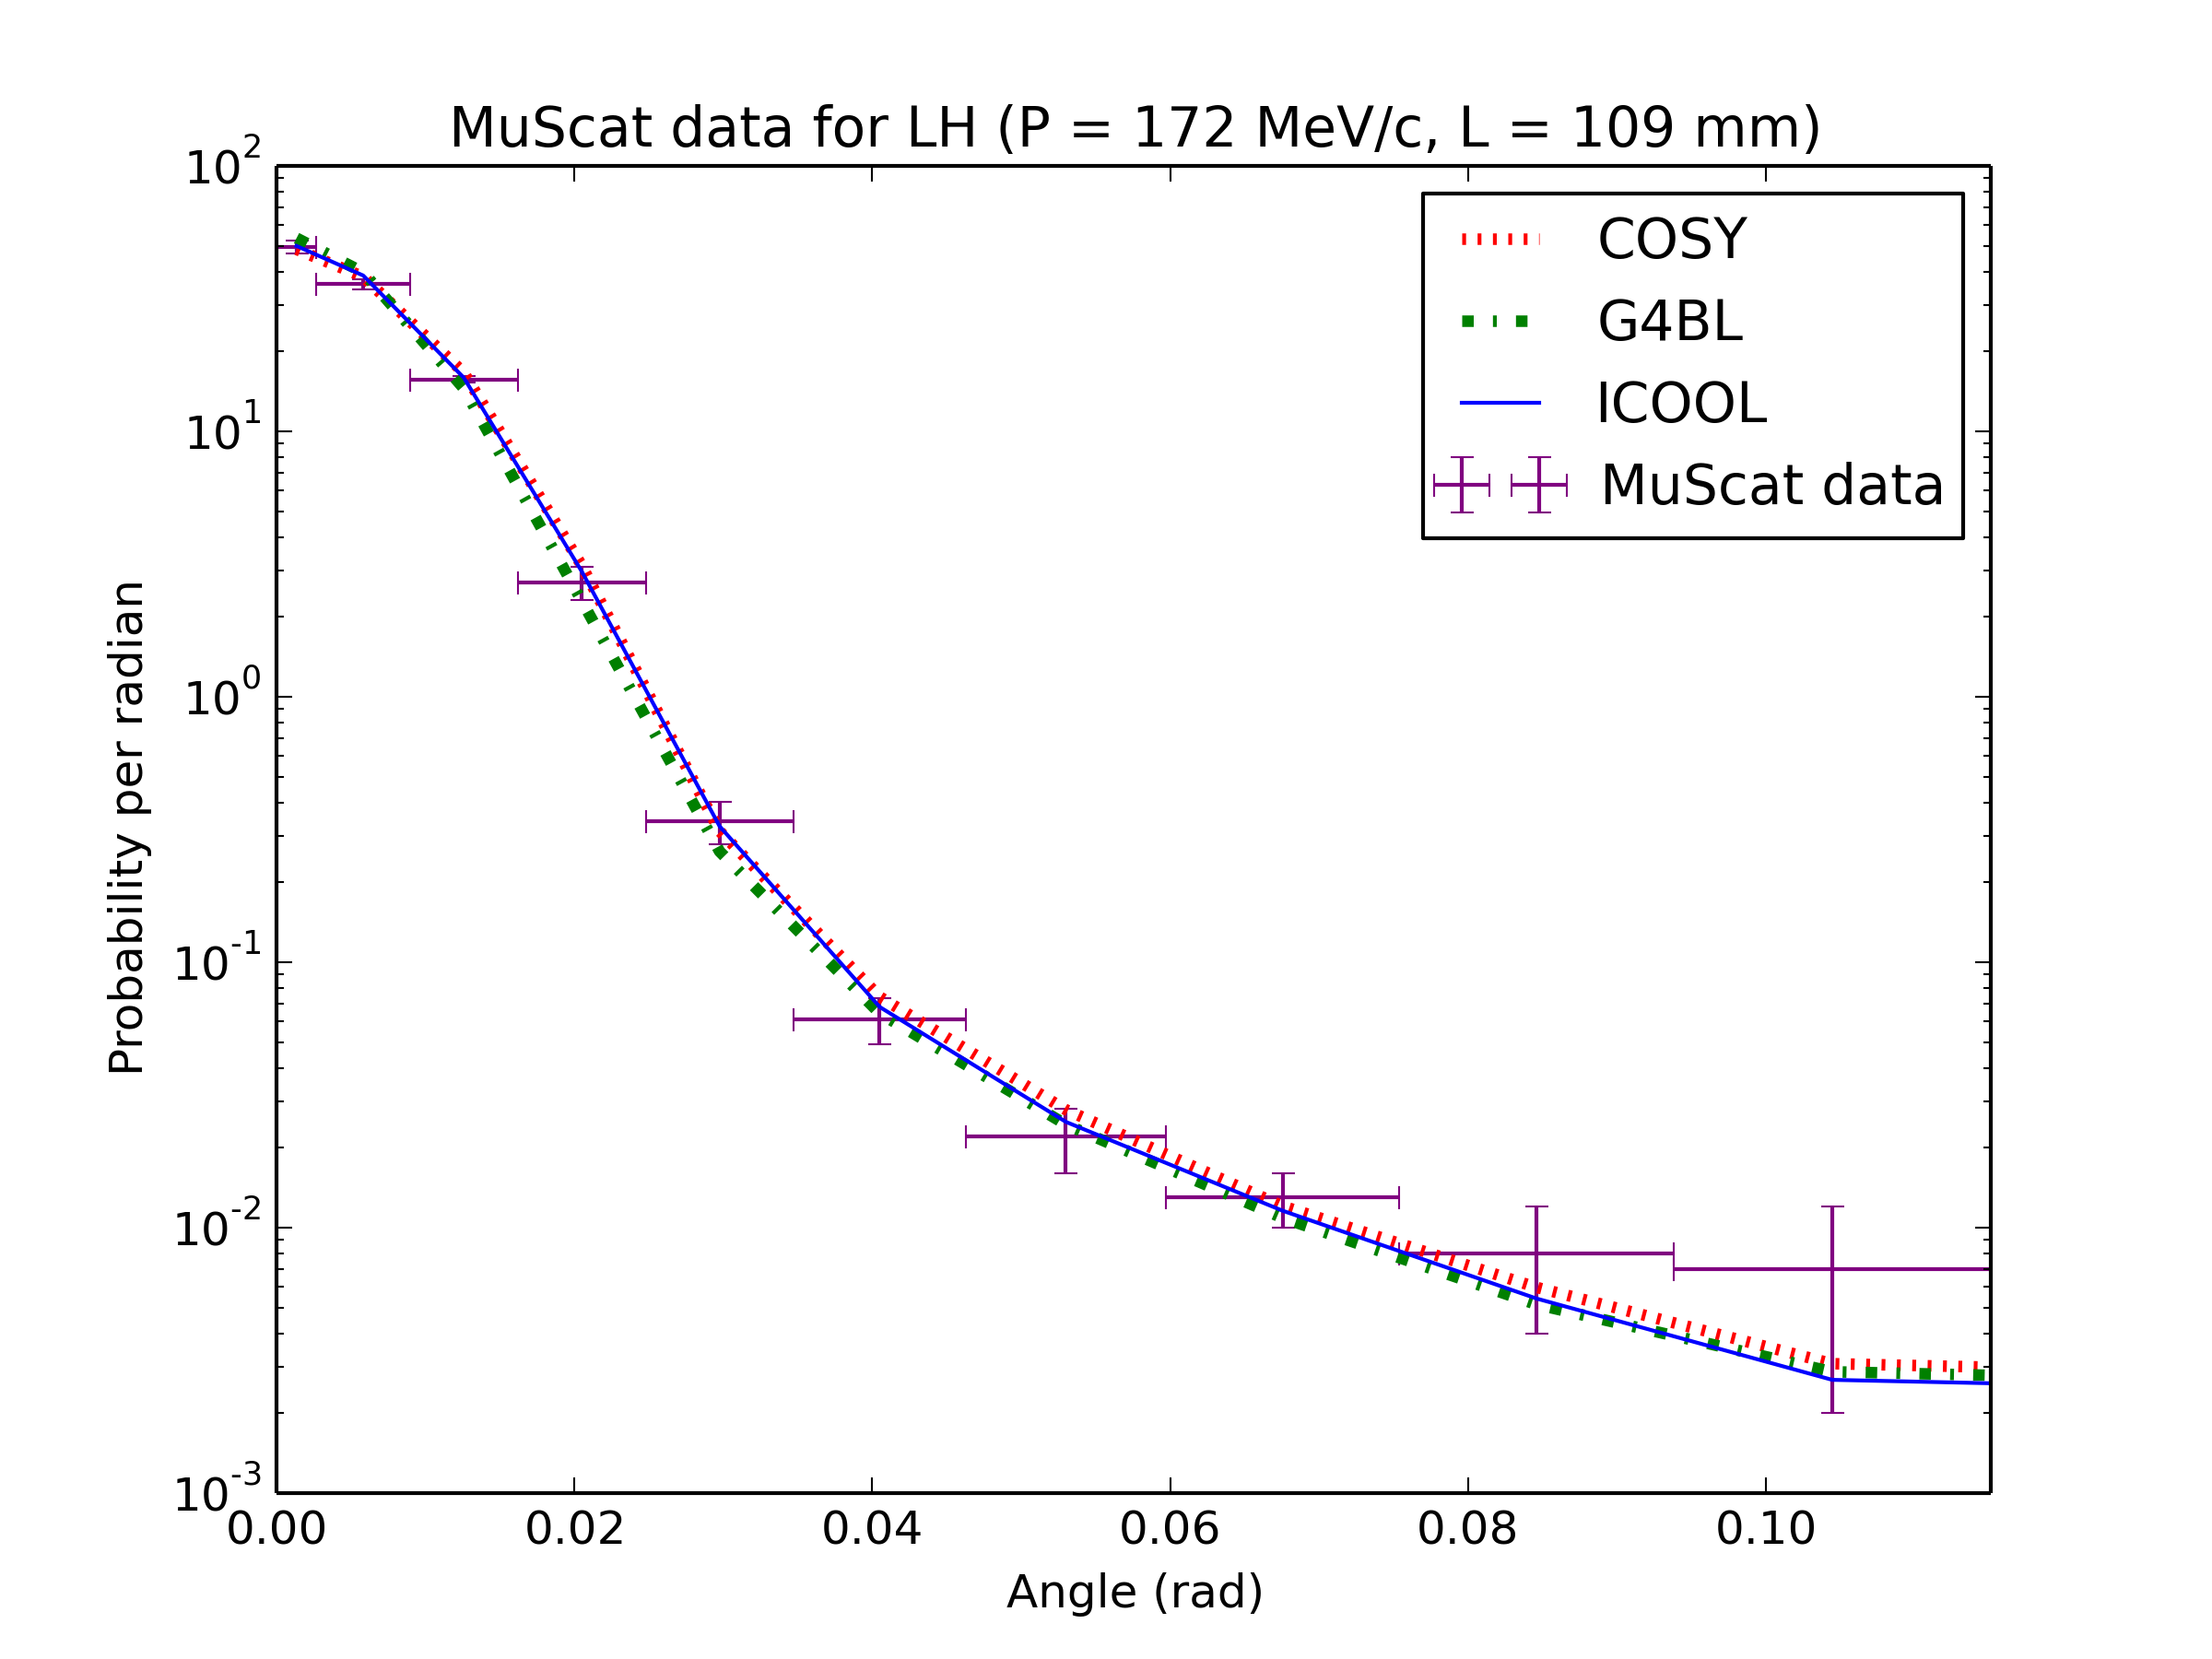
\includegraphics[width=\textwidth]{Figures/172.109.muscat} 
  \caption{MuScat angular scattering results for 109 mm of liquid hydrogen compared against COSY (red), G4BL (green), and ICOOL (blue).}
  \label{fig:172.109.muscat}
\end{figure}

\begin{figure}[H]
  \centering
    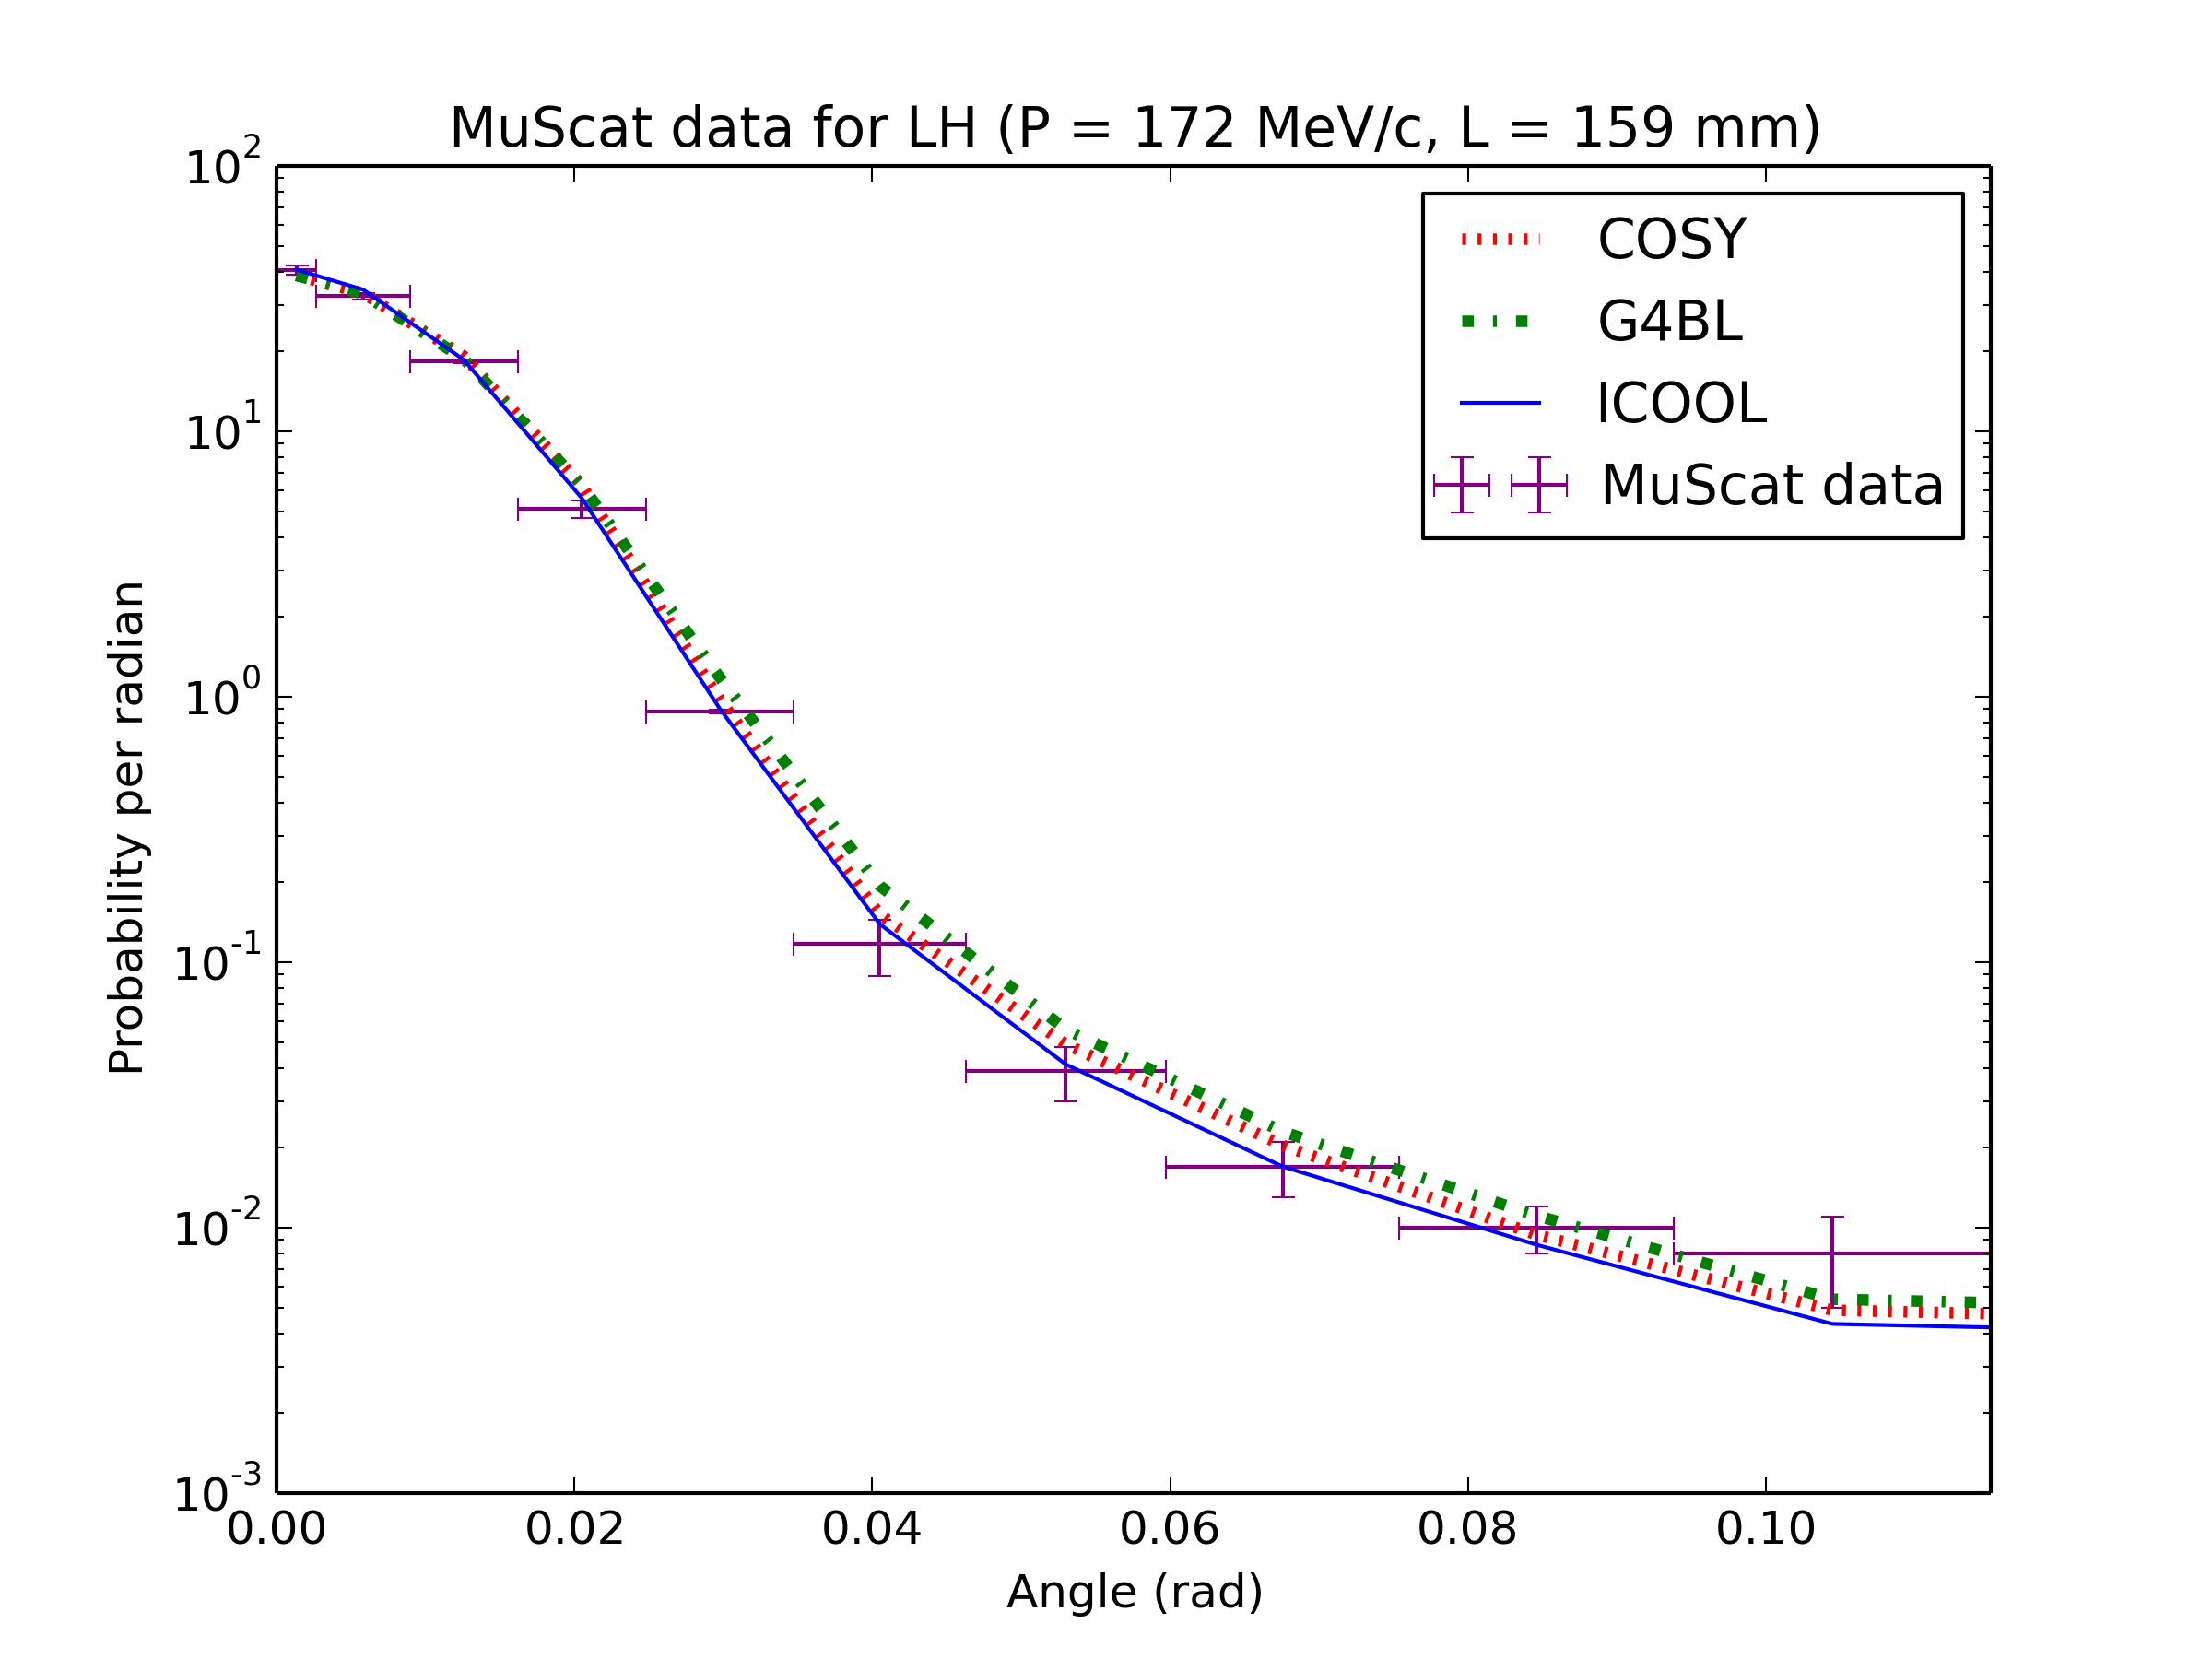
\includegraphics[width=\textwidth]{Figures/172.159.muscat} 
  \caption{MuScat angular scattering results for 159 mm of liquid hydrogen compared against COSY (red), G4BL (green), and ICOOL (blue).}
  \label{fig:172.159.muscat}
\end{figure}

\begin{figure}[H]
  \centering
    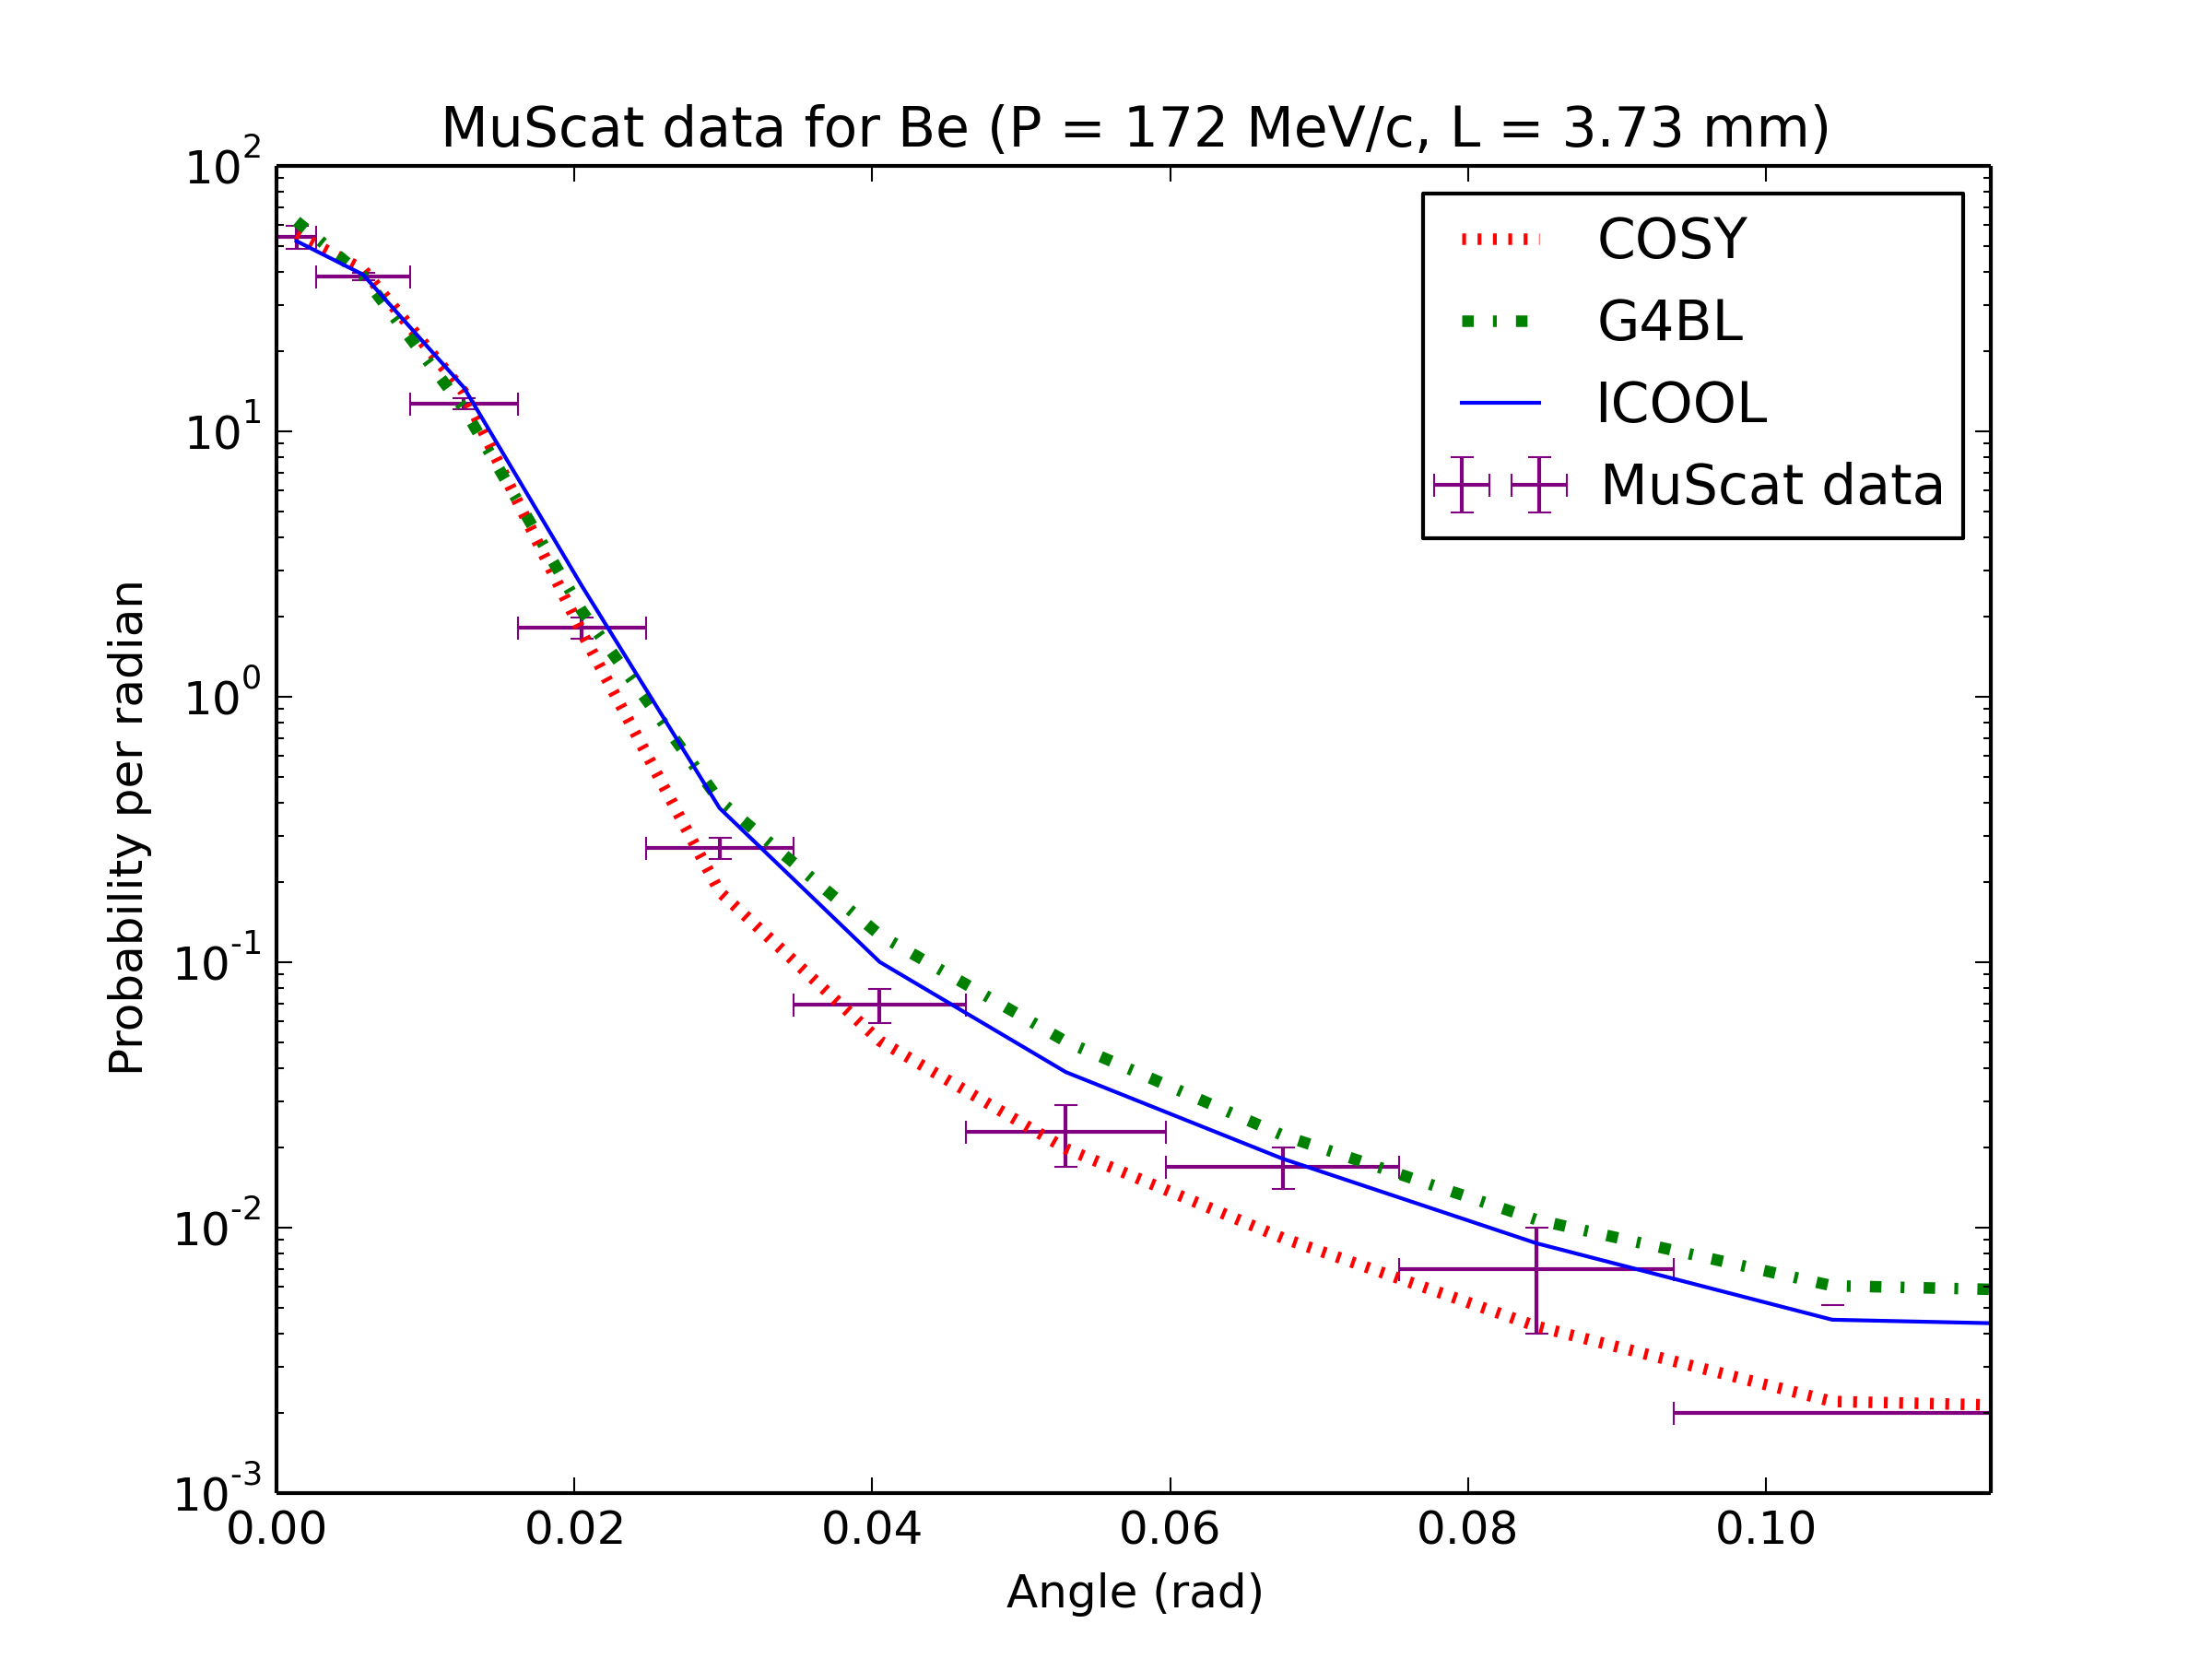
\includegraphics[width=\textwidth]{Figures/172.3.73.muscat} 
  \caption{MuScat angular scattering results for 3.73 mm of beryllium compared against COSY (red), G4BL (green), and ICOOL (blue).}
  \label{fig:172.3.73.muscat}
\end{figure}

In the liquid hydrogen cases, COSY appears to match both G4Beamline and ICOOL very well, as well as the MuScat data points. ICOOL appears to have a sharper peak than either COSY or G4Beamline, which can be more easily seen in the 159 mm liquid hydrogen case than in the 109 mm case. In the case of beryllium, COSY matches the MuScat points slightly better than G4Beamline and ICOOL, particularly for the two data points between 0.04 and 0.06 radians.

\Section{The Muon Ionization Cooling Experiment}\label{sec:mice}

This section introduces the Muon Ionization Cooling Experiment (MICE, \cite{mice}), a practical application for the new absorber routines in COSY. The results of MICE simulations in ICOOL, G4Beamline, and COSY are examined, showing good agreement.

\Subsection{Introduction to MICE}\label{ssc:miceIntro}
The Muon Ionization Cooling Experiment (MICE \cite{mice}) is an experiment currently being developed at the Rutherford Appleton Laboratory in Oxfordshire, U.K. Its goal is to show a proof-of-principle demonstration of muon ionization cooling. MICE Step IV configuration is explored in this work. The Step IV cell includes 12 magnetic coils positioned symmetrically around a flat absorber. Figure~\ref{fig:miceStepIV} shows a schematic of this lattice with 350 mm of liquid hydrogen as the absorber.
\begin{figure}[h!]
  \centering
    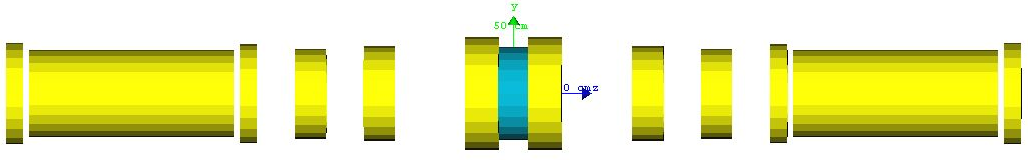
\includegraphics[width=\textwidth]{Figures/miceStepIV} 
  \caption[MICE Step IV cell.]{MICE Step IV cell. Magnetic coils are shown in yellow and the absorber is shown in blue. The green and blue axes are the $y$ and $z$ axes, here drawn to scale as 500 mm each. The aperture (invisible for display purposes) is 300 mm. Image rendered via G4Beamline \cite{g4bl}.}
  \label{fig:miceStepIV}
\end{figure}

\Subsection{Results of MICE Simulation}\label{ssc:miceResults}
$10^6$ muons were simulated through the cell in Figure~\ref{fig:miceStepIV}. The coil parameters may be found in Table~\ref{tbl:MICE_coil_parameters}. The absorber was a 350 mm cylindrical block of liquid hydrogen centered at $z=0$. The aperture was set to 300 mm. Note that other materials such as safety windows were not accounted for in this simulation. The decay process was disabled in all simulation codes. The beam started at $-$2.45105 m and ended at 2.450 m. The initial distribution was Gaussian with parameters summarized in Table~\ref{tbl:MICE_initial_distribution_parameters}.

\begin{table}
\caption*{\textbf{MICE Step IV Coil Parameters}}
\begin{tabularx}{\textwidth}{cccccccc}
\hline \hline
Name & $z$ position & Length & Inner radius & Outer radius & Current density  \vspace{-12pt}\\
 & mm & mm & mm & mm & A/mm$^2$  \\
\hline
	End2 & $\mp$3200.28&110.642&258&325.783&$\pm$126 \vspace{-12pt}\\
	Center&$\mp$2450.275&1314.3&258&280.125&$\pm$148 \vspace{-12pt}\\
	End1 & $\mp$1700.29& 110.642& 258 & 318.905 & $\pm$133 \vspace{-12pt}\\
	Match2 & $\mp$1300.29 & 199.492 & 258 & 288.925 & $\pm$132 \vspace{-12pt}\\
	Match1 & $\mp$860.645 & 201.268 & 258 & 304.165 & $\pm133$ \vspace{-12pt}\\
	Focus & $\mp$202.2 & 213.3 & 267.6 & 361.9 & $\pm$104 \\ 
\hline
\end{tabularx}
\caption[MICE Step IV coil parameters.]{MICE Step IV coil parameters corresponding to Figure~\ref{fig:miceStepIV}.}
\label{tbl:MICE_coil_parameters}
\end{table}

%\newcolumntype{A}{ >{\centering\arraybackslash} m{2.5cm} } 
\begin{table}
\caption*{\textbf{MICE Step IV Initial Distribution Parameters}}
\begin{center}
\begin{tabularx}{0.7\textwidth}{p{1cm}ccc}
\hline \hline
&Parameter & Mean & Standard deviation \\
\hline
	&$x$ (mm) & 0 & 32\vspace{-12pt}\\
	&$y$ (mm) & 0 & 32\vspace{-12pt} \\
	&$z$ (mm) & 0 & 0\vspace{-12pt} \\
	&$p_x$ (MeV/$c$) & 0 & 20\vspace{-12pt} \\
	&$p_y$ (MeV/$c$) & 0 & 20\vspace{-12pt} \\
	&$p_z$ (MeV/$c$) & 200 & 30\\
\hline
\end{tabularx}
\end{center}
\caption{MICE Step IV initial distribution Gaussian parameters.}
\label{tbl:MICE_initial_distribution_parameters}
\end{table}

While the selection of order and step size is detailed in the next section, it was found that a 5th order simulation was sufficient for COSY. Through the coil-only portion of the simulation, 50 steps were taken on each side of the absorber (or roughly a step size of 46 mm both upstream and downstream). The particles were tracked through the momentary transfer map after each step and then the transfer map was set to unity. It was noted that for the coil-only section, a single transfer map was not sufficient even at the 9th order. This is due to the relatively large phase space volume of the beam and the complexity of the magnetic field. Through the absorber-coil region ($-$350/2 mm to 350/2 mm), it was found that a 1st order map with 5 steps was sufficient. This is due to the transverse phase space of the beam reaching a minimum and the magnetic field passing through the point of symmetry.

Compounding the map without propagating the beam also gave poor results. When one takes the composition of two $n^{th}$ order transfer maps, a transfer map of order $n\times n$ is the result. For example, the first step in MICE simulation would yield a 5th order transfer map. Taking the second step would give a new transfer map of order $5\times 5 = 25$. However, since COSY is operating in the 5th order mode, the new transfer map would not be 25th order, but rather it would be truncated to a 5th order map. For this reason, the particles were propagated through the momentary transfer map after each step in the simulation.

The magnetic field in G4Beamline was created using the \texttt{coil} and \texttt{solenoid} commands. The field was then exported to a file using the \texttt{printfield} command to a file. The field map file was read by both G4Beamline (which used the \texttt{fieldmap} command) and ICOOL (which used the \texttt{GRID} command operating in \texttt{G43D} mode).

\begin{figure}[H]
  \centering
    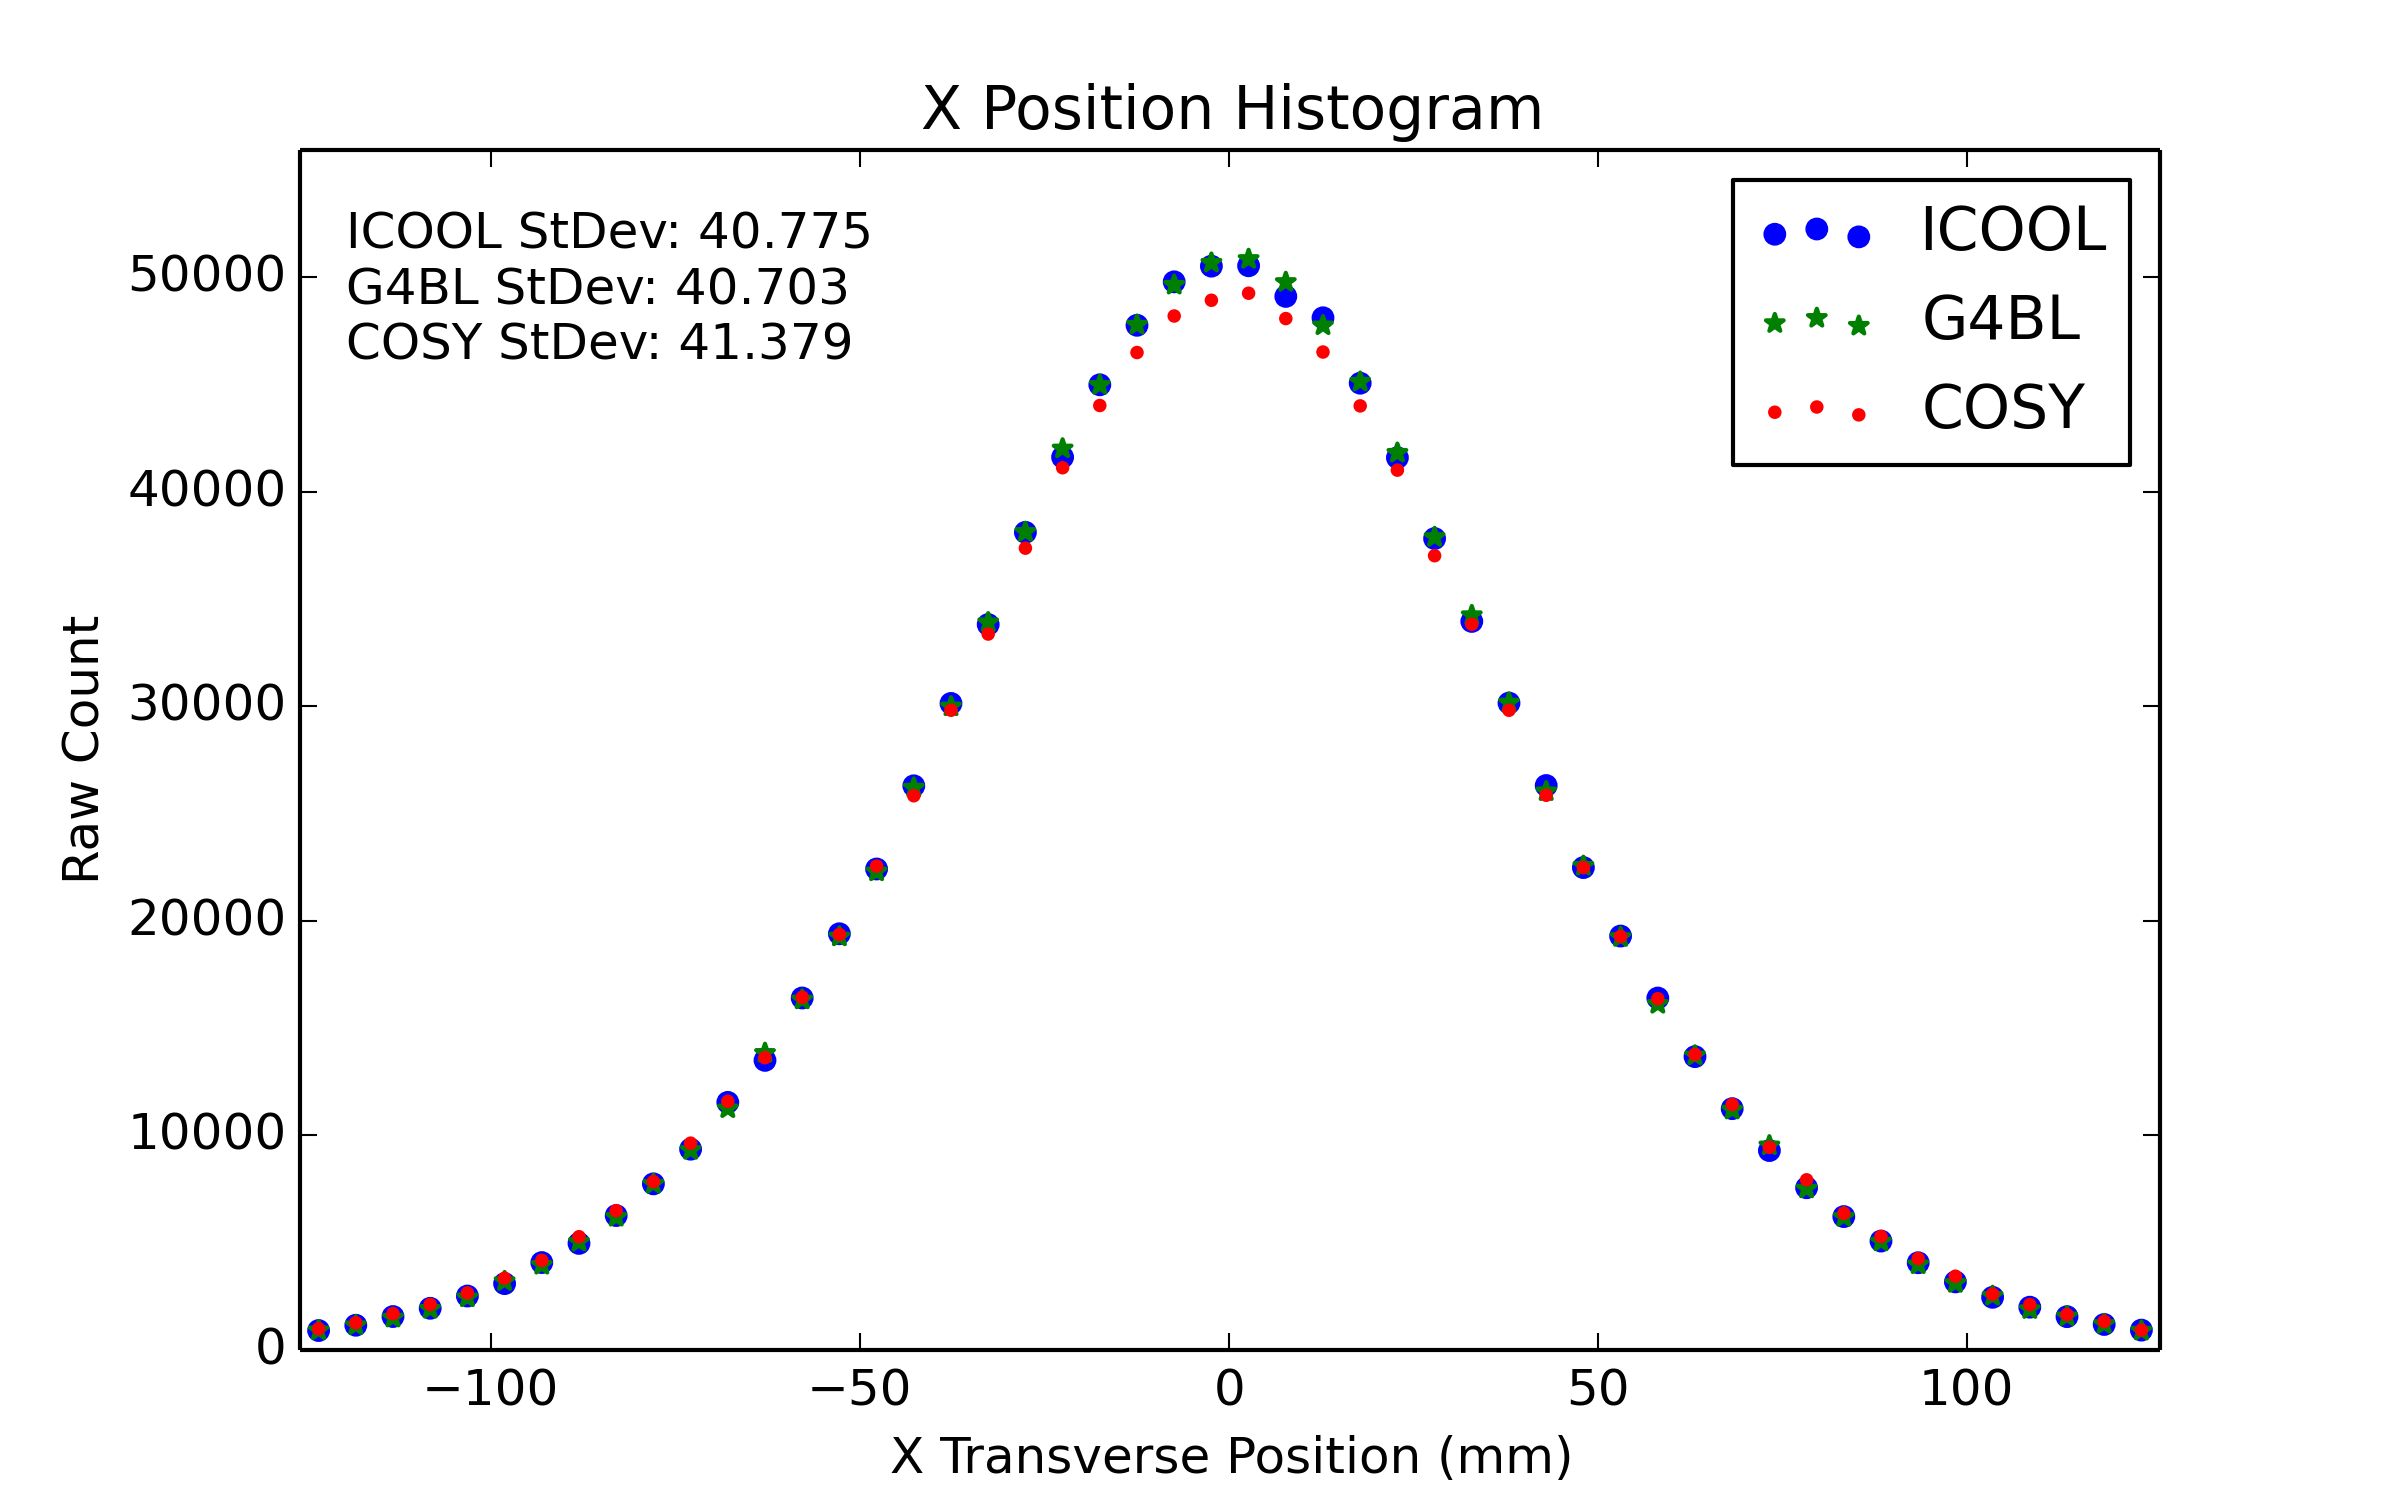
\includegraphics[width=\textwidth]{MICE data/x} 
  \caption{MICE Step IV $x$ position results for 350 mm of liquid hydrogen.}
  \label{fig:micex}
\end{figure}

\begin{figure}[H]
  \centering
    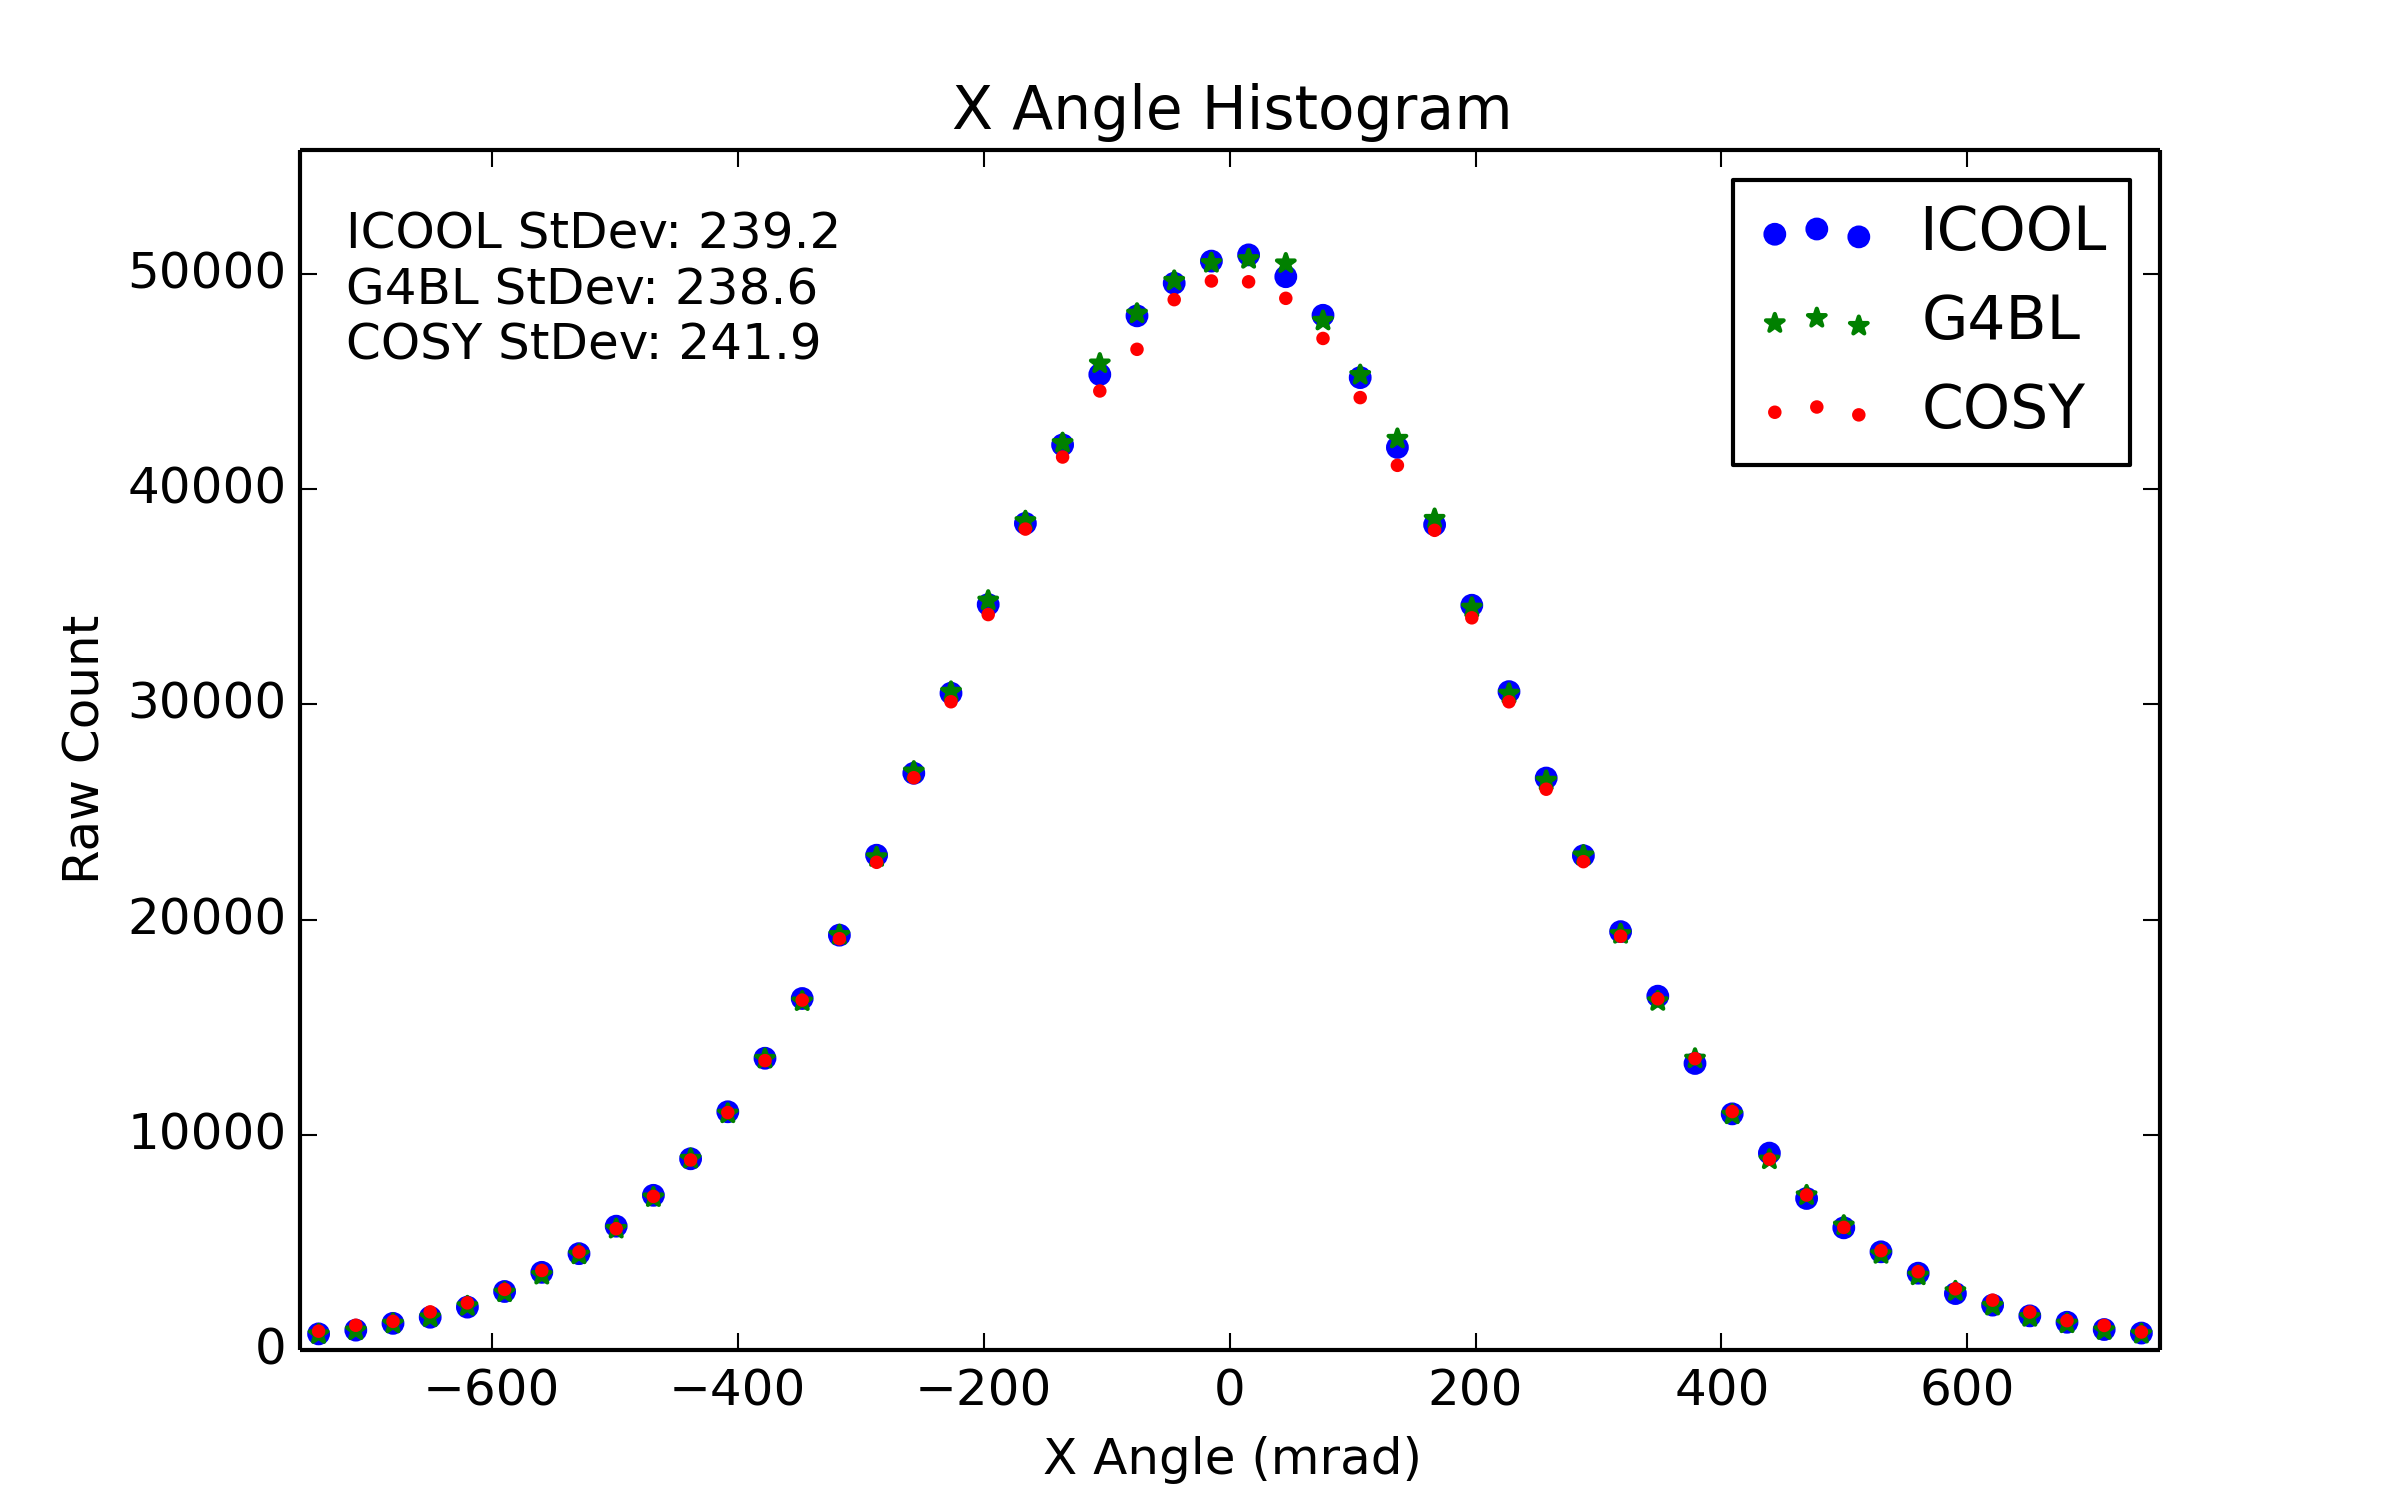
\includegraphics[width=\textwidth]{MICE data/px} 
  \caption{MICE Step IV $x$ angle results for 350 mm of liquid hydrogen.}
  \label{fig:micexangle}
\end{figure}

\begin{figure}[H]
  \centering
    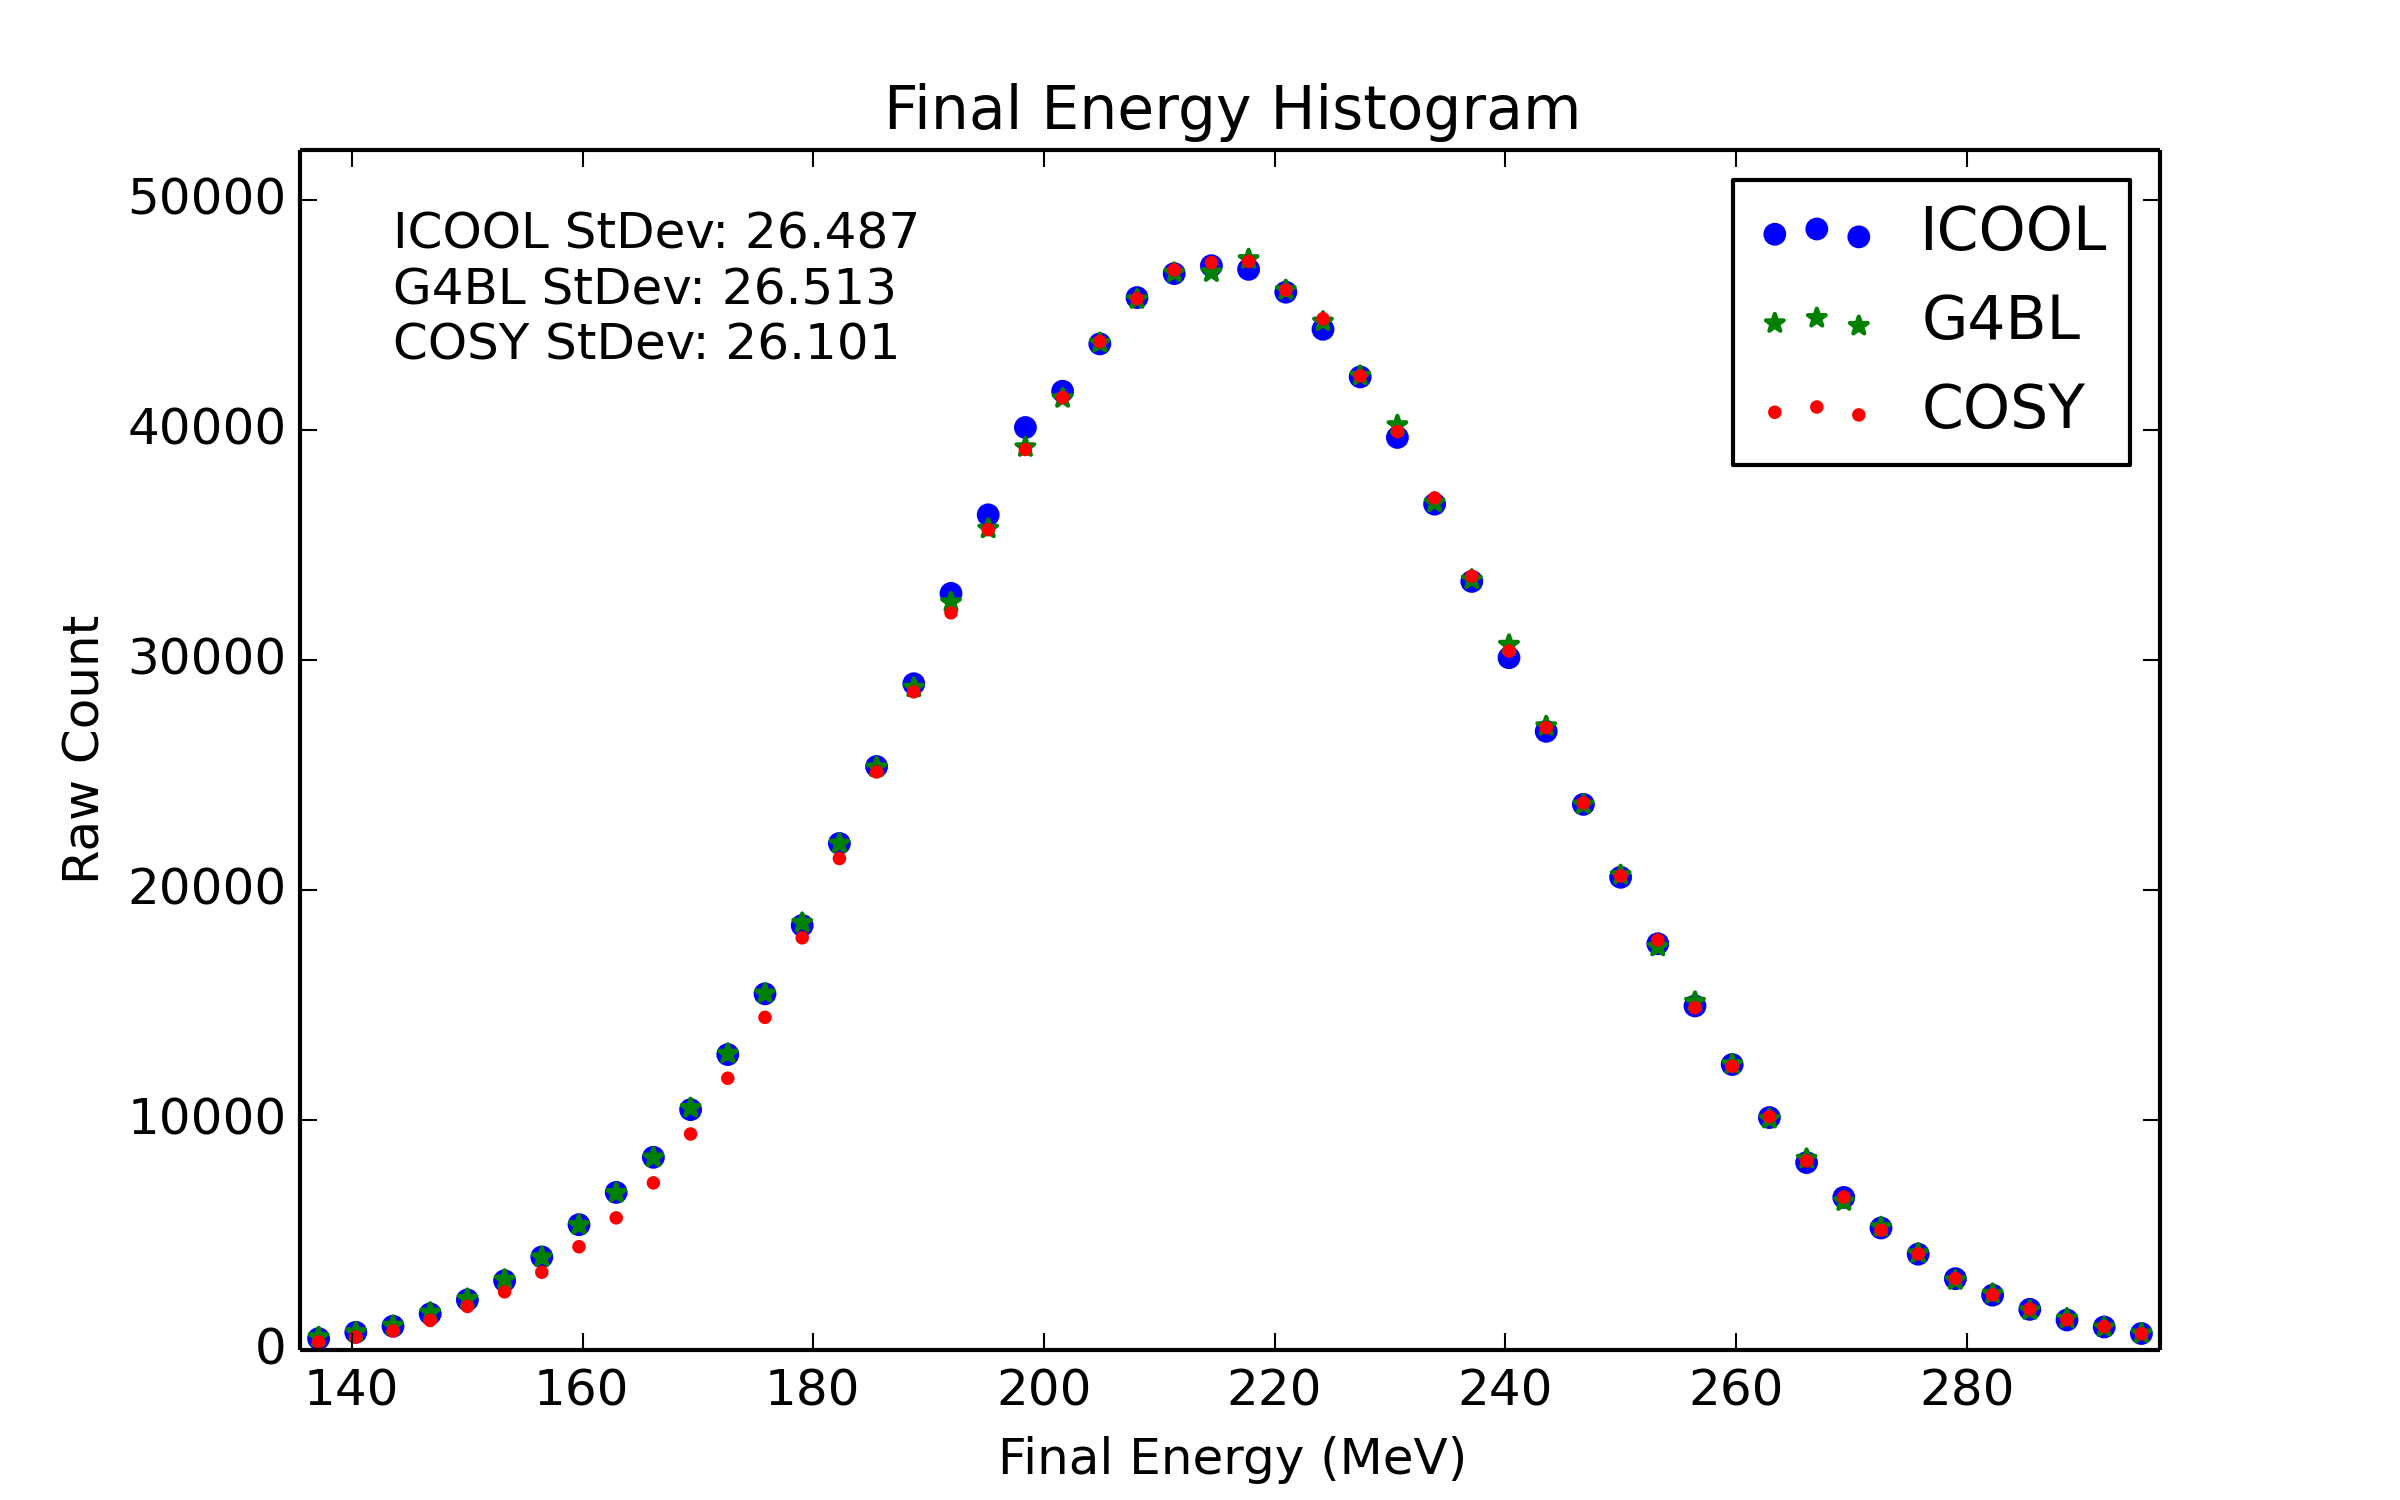
\includegraphics[width=\textwidth]{MICE data/e} 
  \caption{MICE Step IV final energy results for 350 mm of liquid hydrogen.}
  \label{fig:miceenergy}
\end{figure}

The runtimes of ICOOL, G4Beamline, and COSY are listed in Table~\ref{tbl:mice_times}. To reiterate, COSY was run at 5th order with 50 steps before the absorber, 5 steps at 1st order inside the absorber, and 50 steps at 5th order after the absorber. Note that the initialization time for G4Beamline to create the field maps was 33 seconds. The time it took to create a text file for ICOOL input was 11 seconds. Since G4Beamline only has to create the field map once, the initialization time is added to neither ICOOL nor G4Beamline the run times in Table~\ref{tbl:mice_times}. COSY did not have any initialization time.

\begin{table}
\caption*{\textbf{Run Times (in seconds) for MICE Step IV Simulation}}
\begin{center}
\begin{tabularx}{0.55\textwidth}{ccccc}
%\vspace{-40pt}\\ 
\hline \hline
Number of particles: & $10^6$ & $10^5$ & $10^4$ & $10^3$\\
\hline
COSY: & 367 & 31 & 6 & 4\vspace{-12pt}\\
G4BL (coils): & 3973 & 392 & 40 & 6\vspace{-12pt}\\
G4BL (field map): & 662 & 75 & 15 & 9\vspace{-12pt}\\
ICOOL (field map): & 1091 & 117 & 19 & 9\\
\hline
\end{tabularx}
\end{center}
\caption[Run times for MICE Step IV simulation.]{Run times for MICE Step IV simulation for liquid hydrogen. Note that the G4Beamline initialization time was not added to the run time values. G4BL (coils) represents the simulation in G4Beamline when the \texttt{coil} parameter was used. G4BL (field map) represents the simulation when G4Beamline (like ICOOL) read the field map from a file.}
\label{tbl:mice_times}
\end{table}

As a second test, MICE configuration in Figure~\ref{fig:miceStepIV} was simulated using 65 mm of lithium hydride. Lithium hydride is an attractive material because, unlike liquid hydrogen, it does not require cryogenic conditions, but still maintains a low $Z$ value. It can be seen from Figures \ref{fig:mice_lih_x}, \ref{fig:mice_lih_xangle}, and \ref{fig:mice_lih_energy} that 65 mm of lithium hydride has a similar effect on the beam as 350 mm of liquid hydrogen.

\begin{figure}[H]
  \centering
    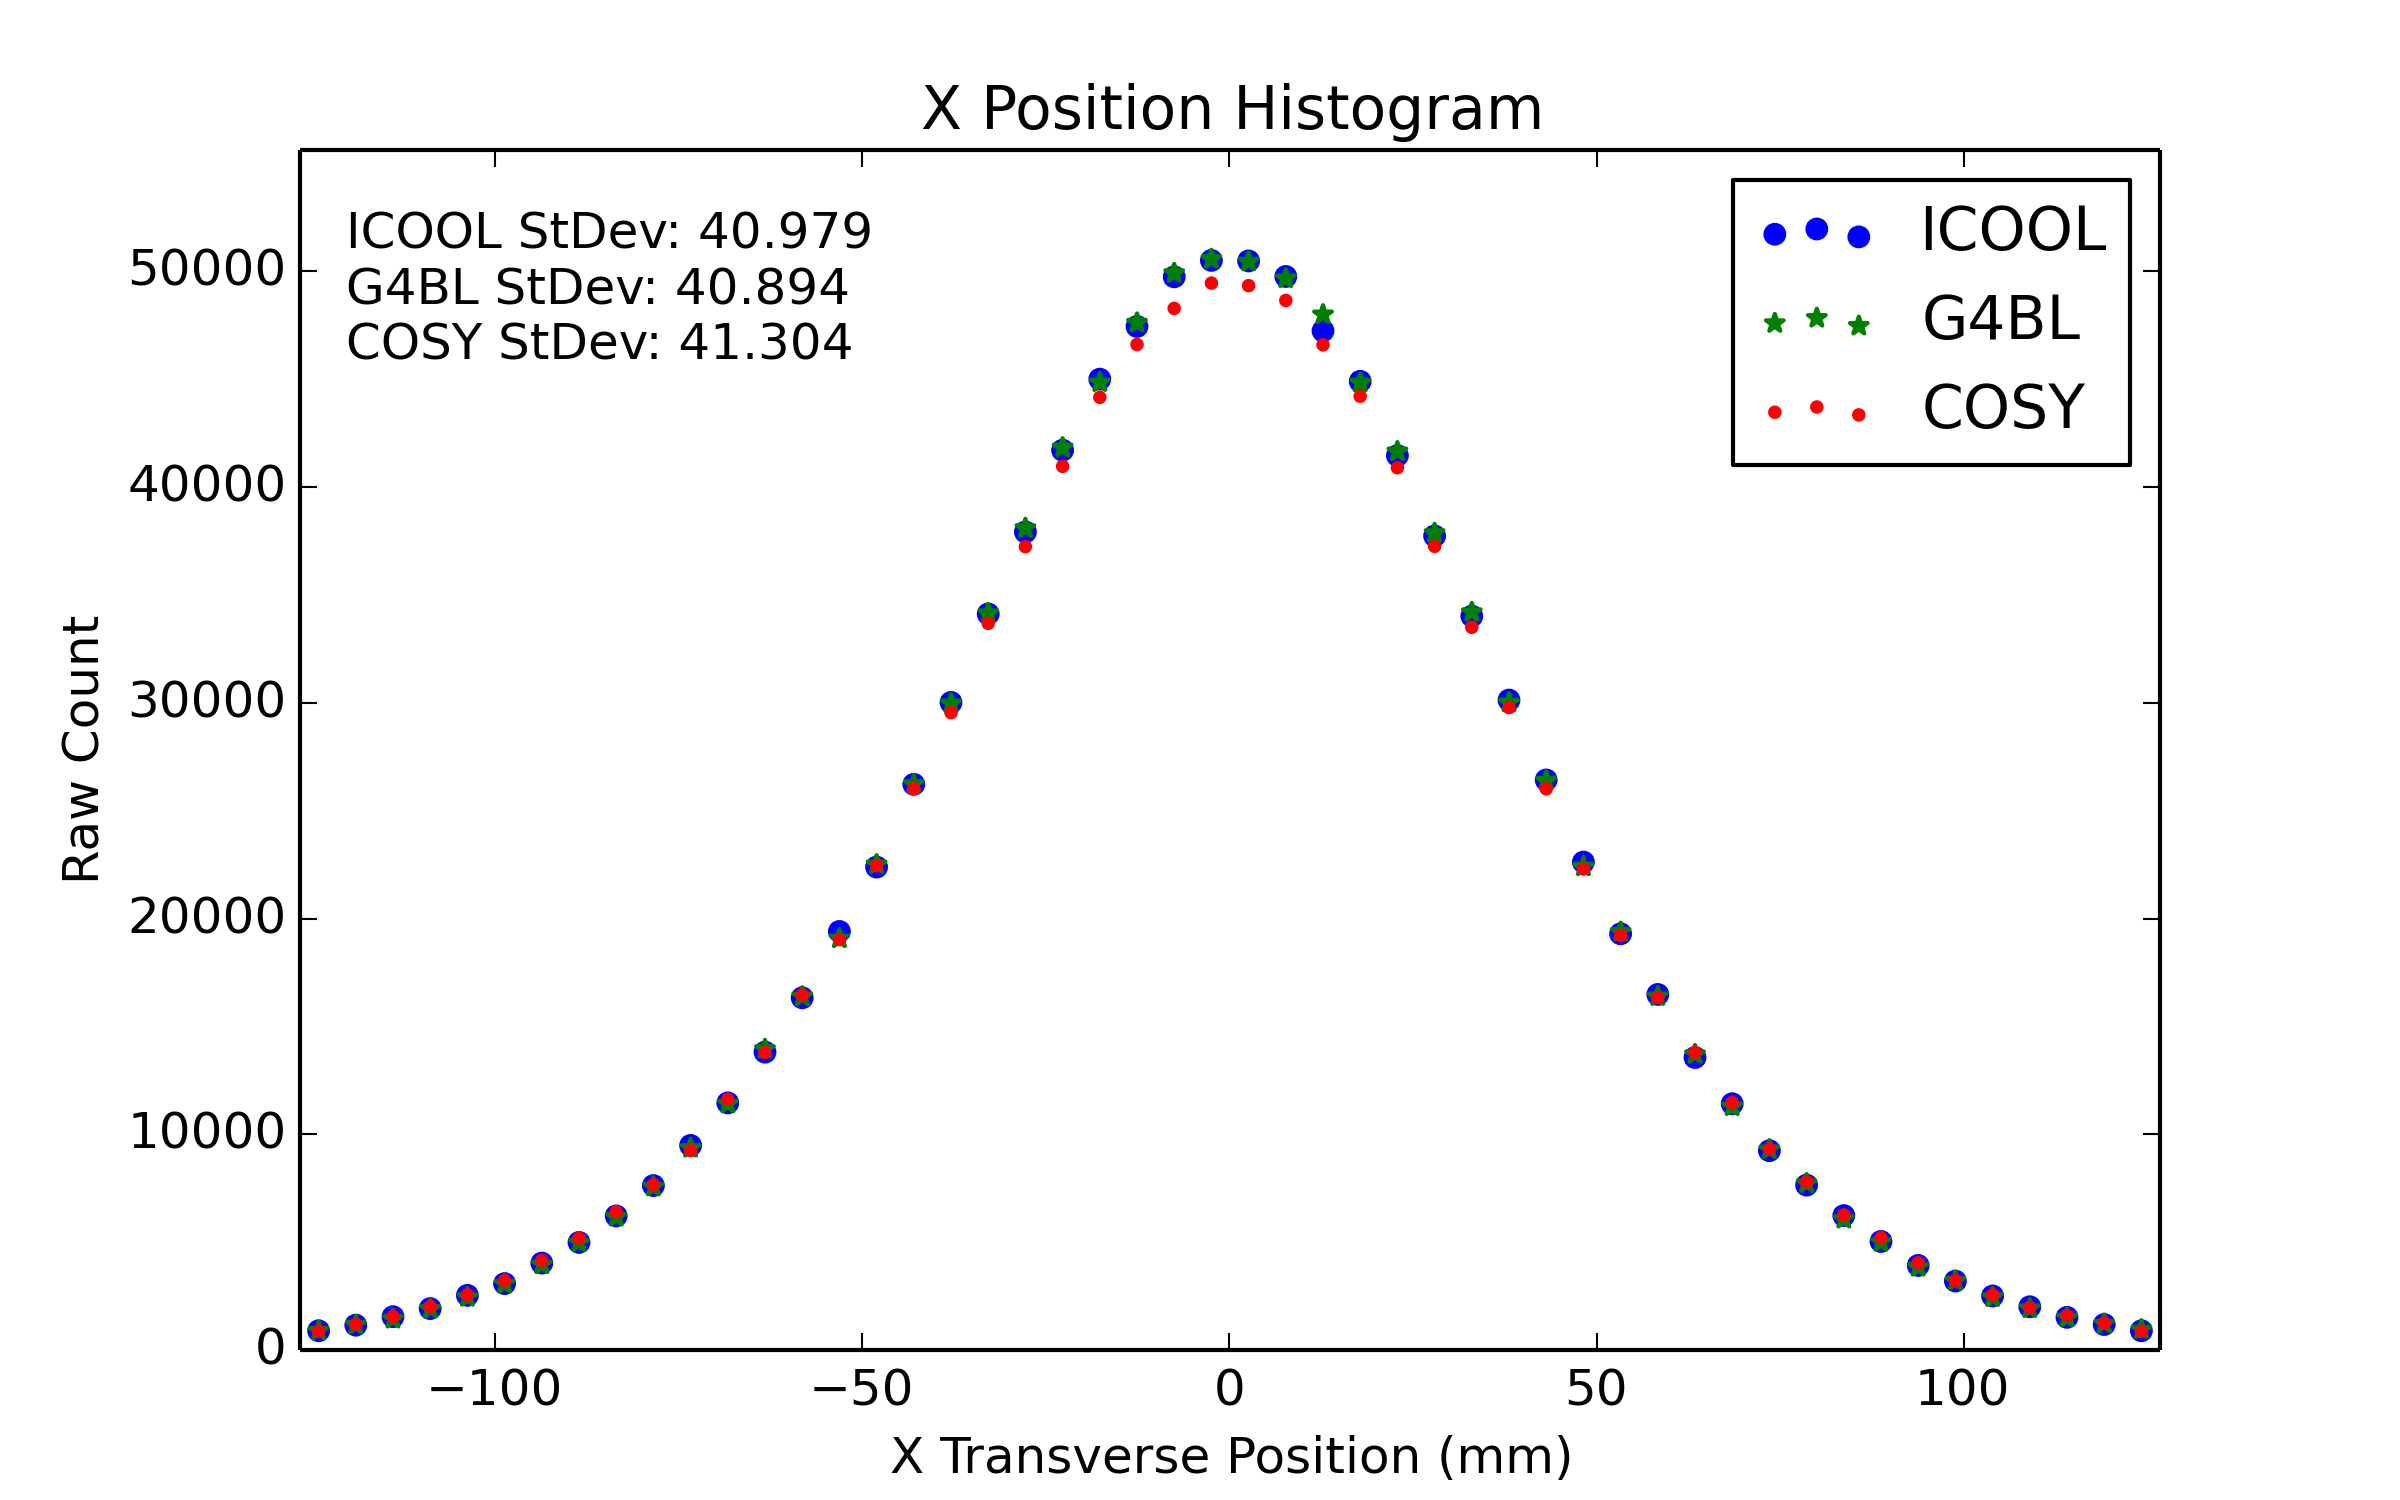
\includegraphics[width=\textwidth]{MICE data/LiH/x} 
  \caption{MICE Step IV $x$ position results for 65 mm of lithium hydride.}
  \label{fig:mice_lih_x}
\end{figure}

\begin{figure}[H]
  \centering
    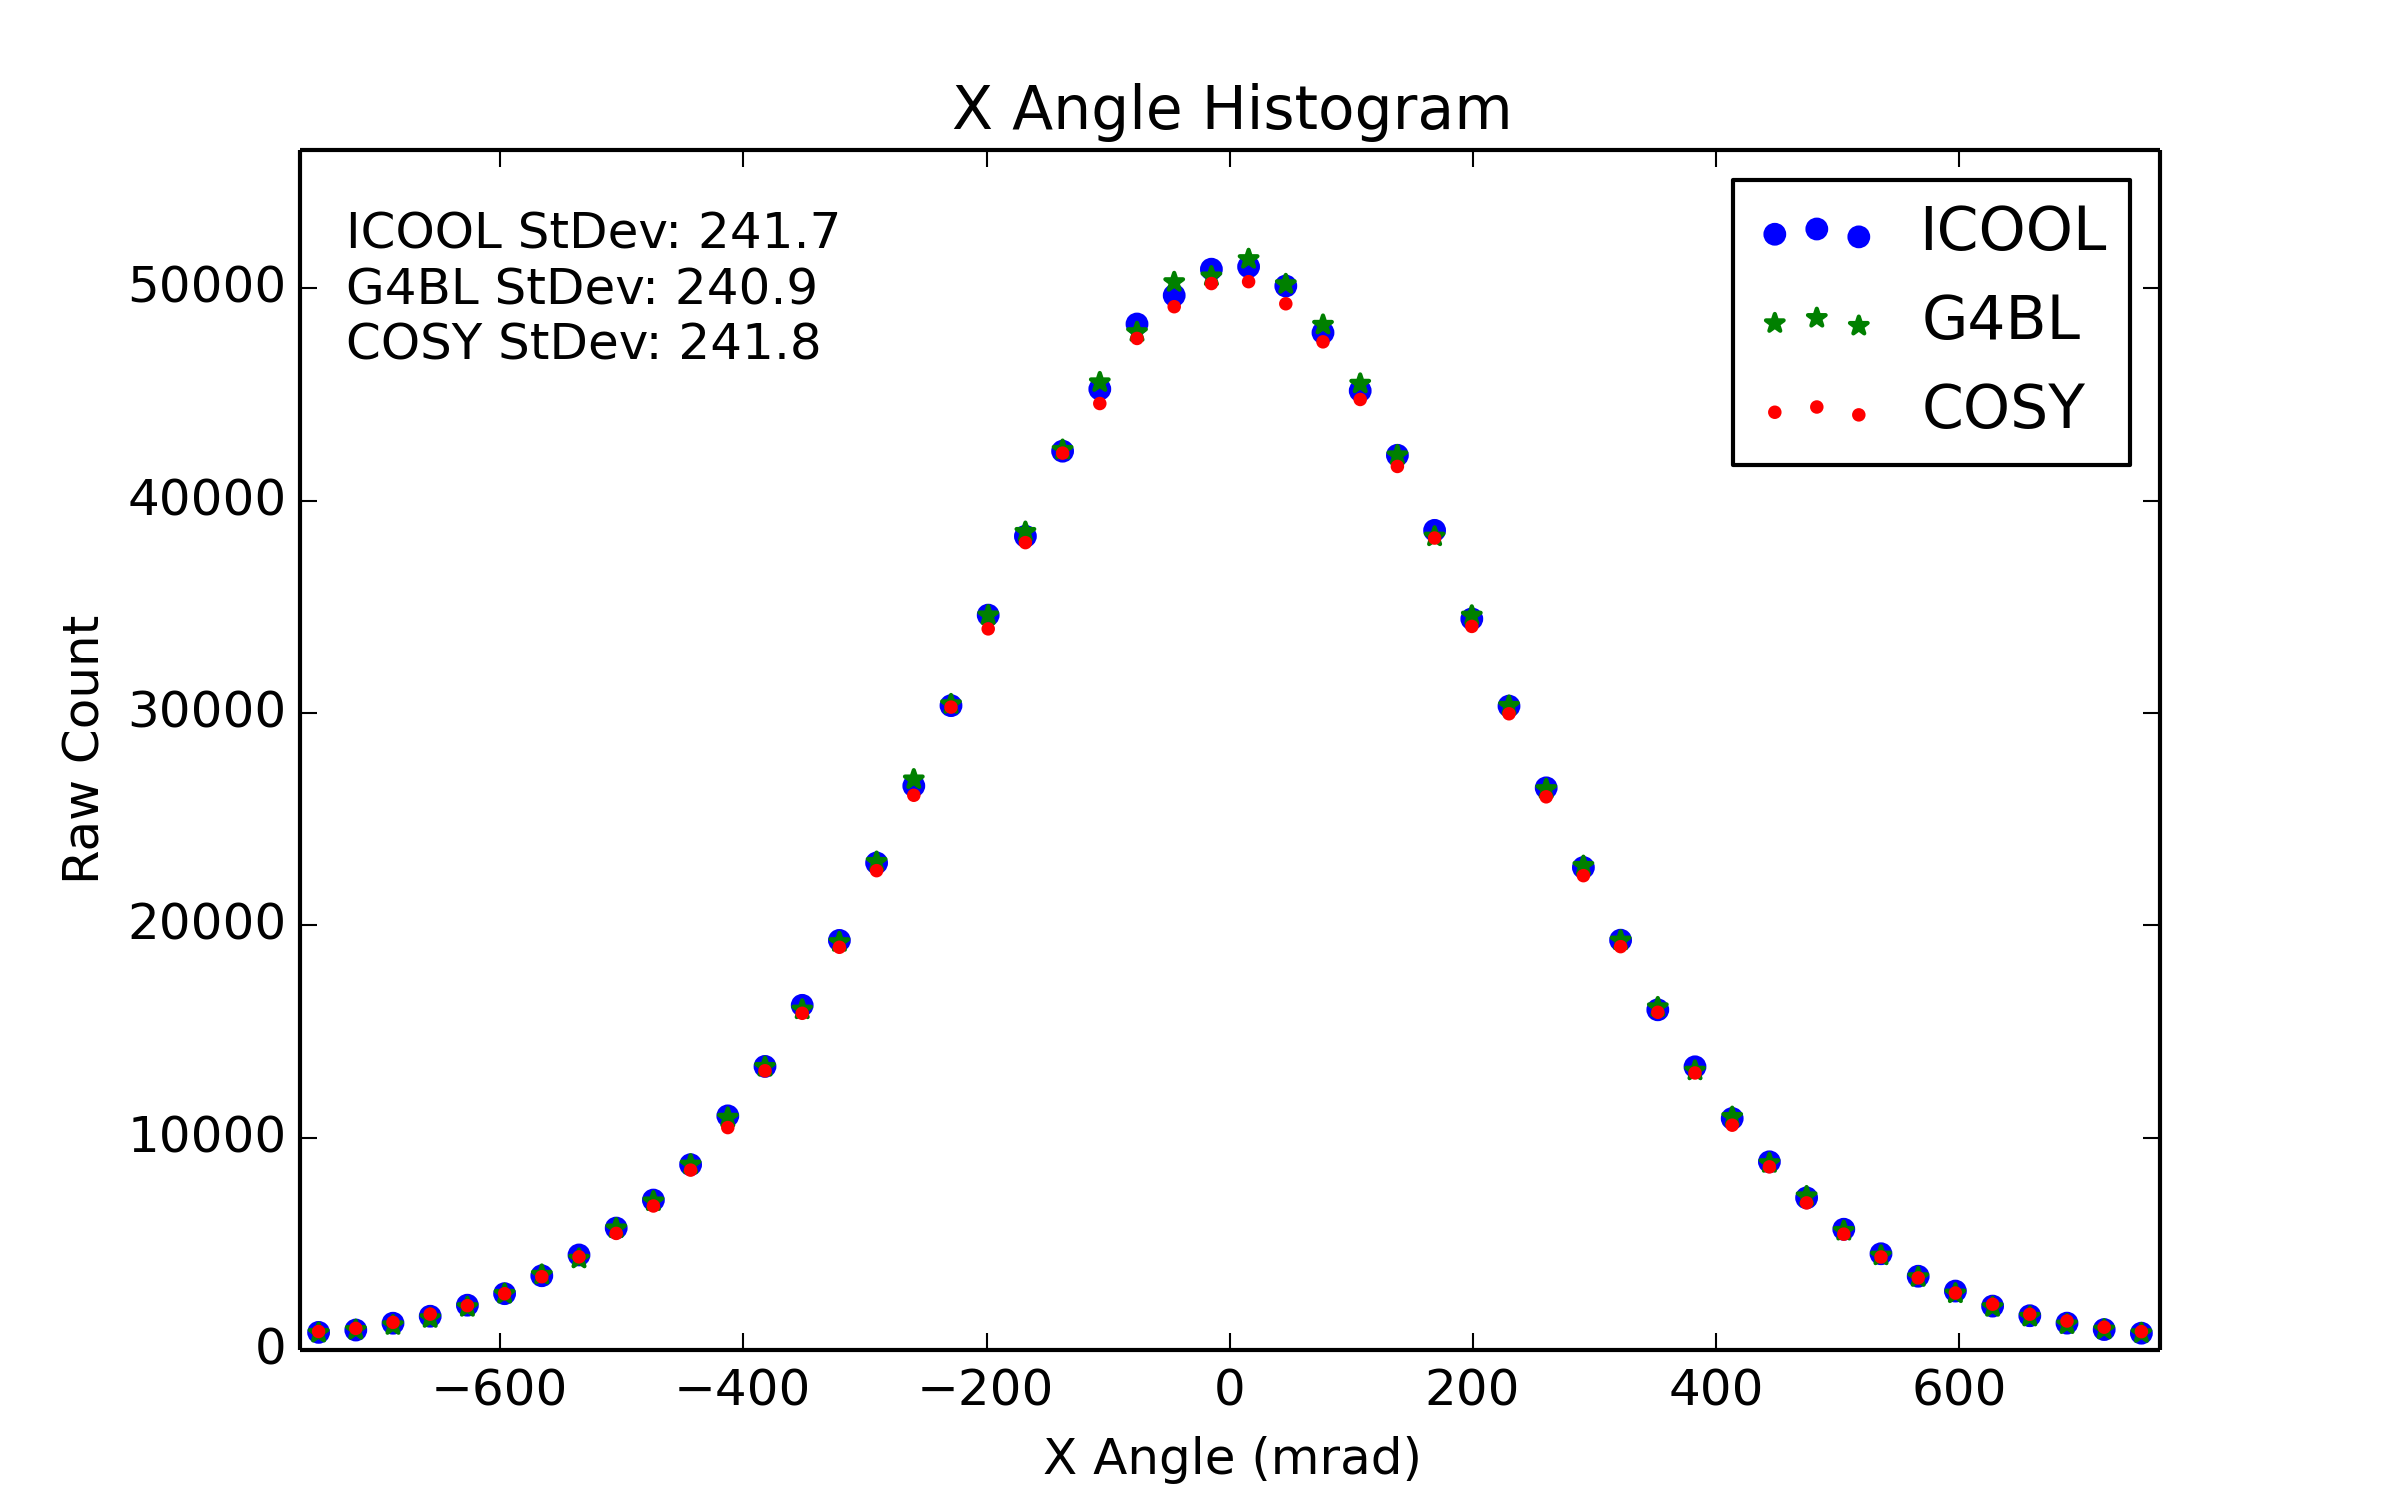
\includegraphics[width=\textwidth]{MICE data/LiH/px} 
  \caption{MICE Step IV $x$ angle results for 65 mm of lithium hydride.}
  \label{fig:mice_lih_xangle}
\end{figure}

\begin{figure}[H]
  \centering
    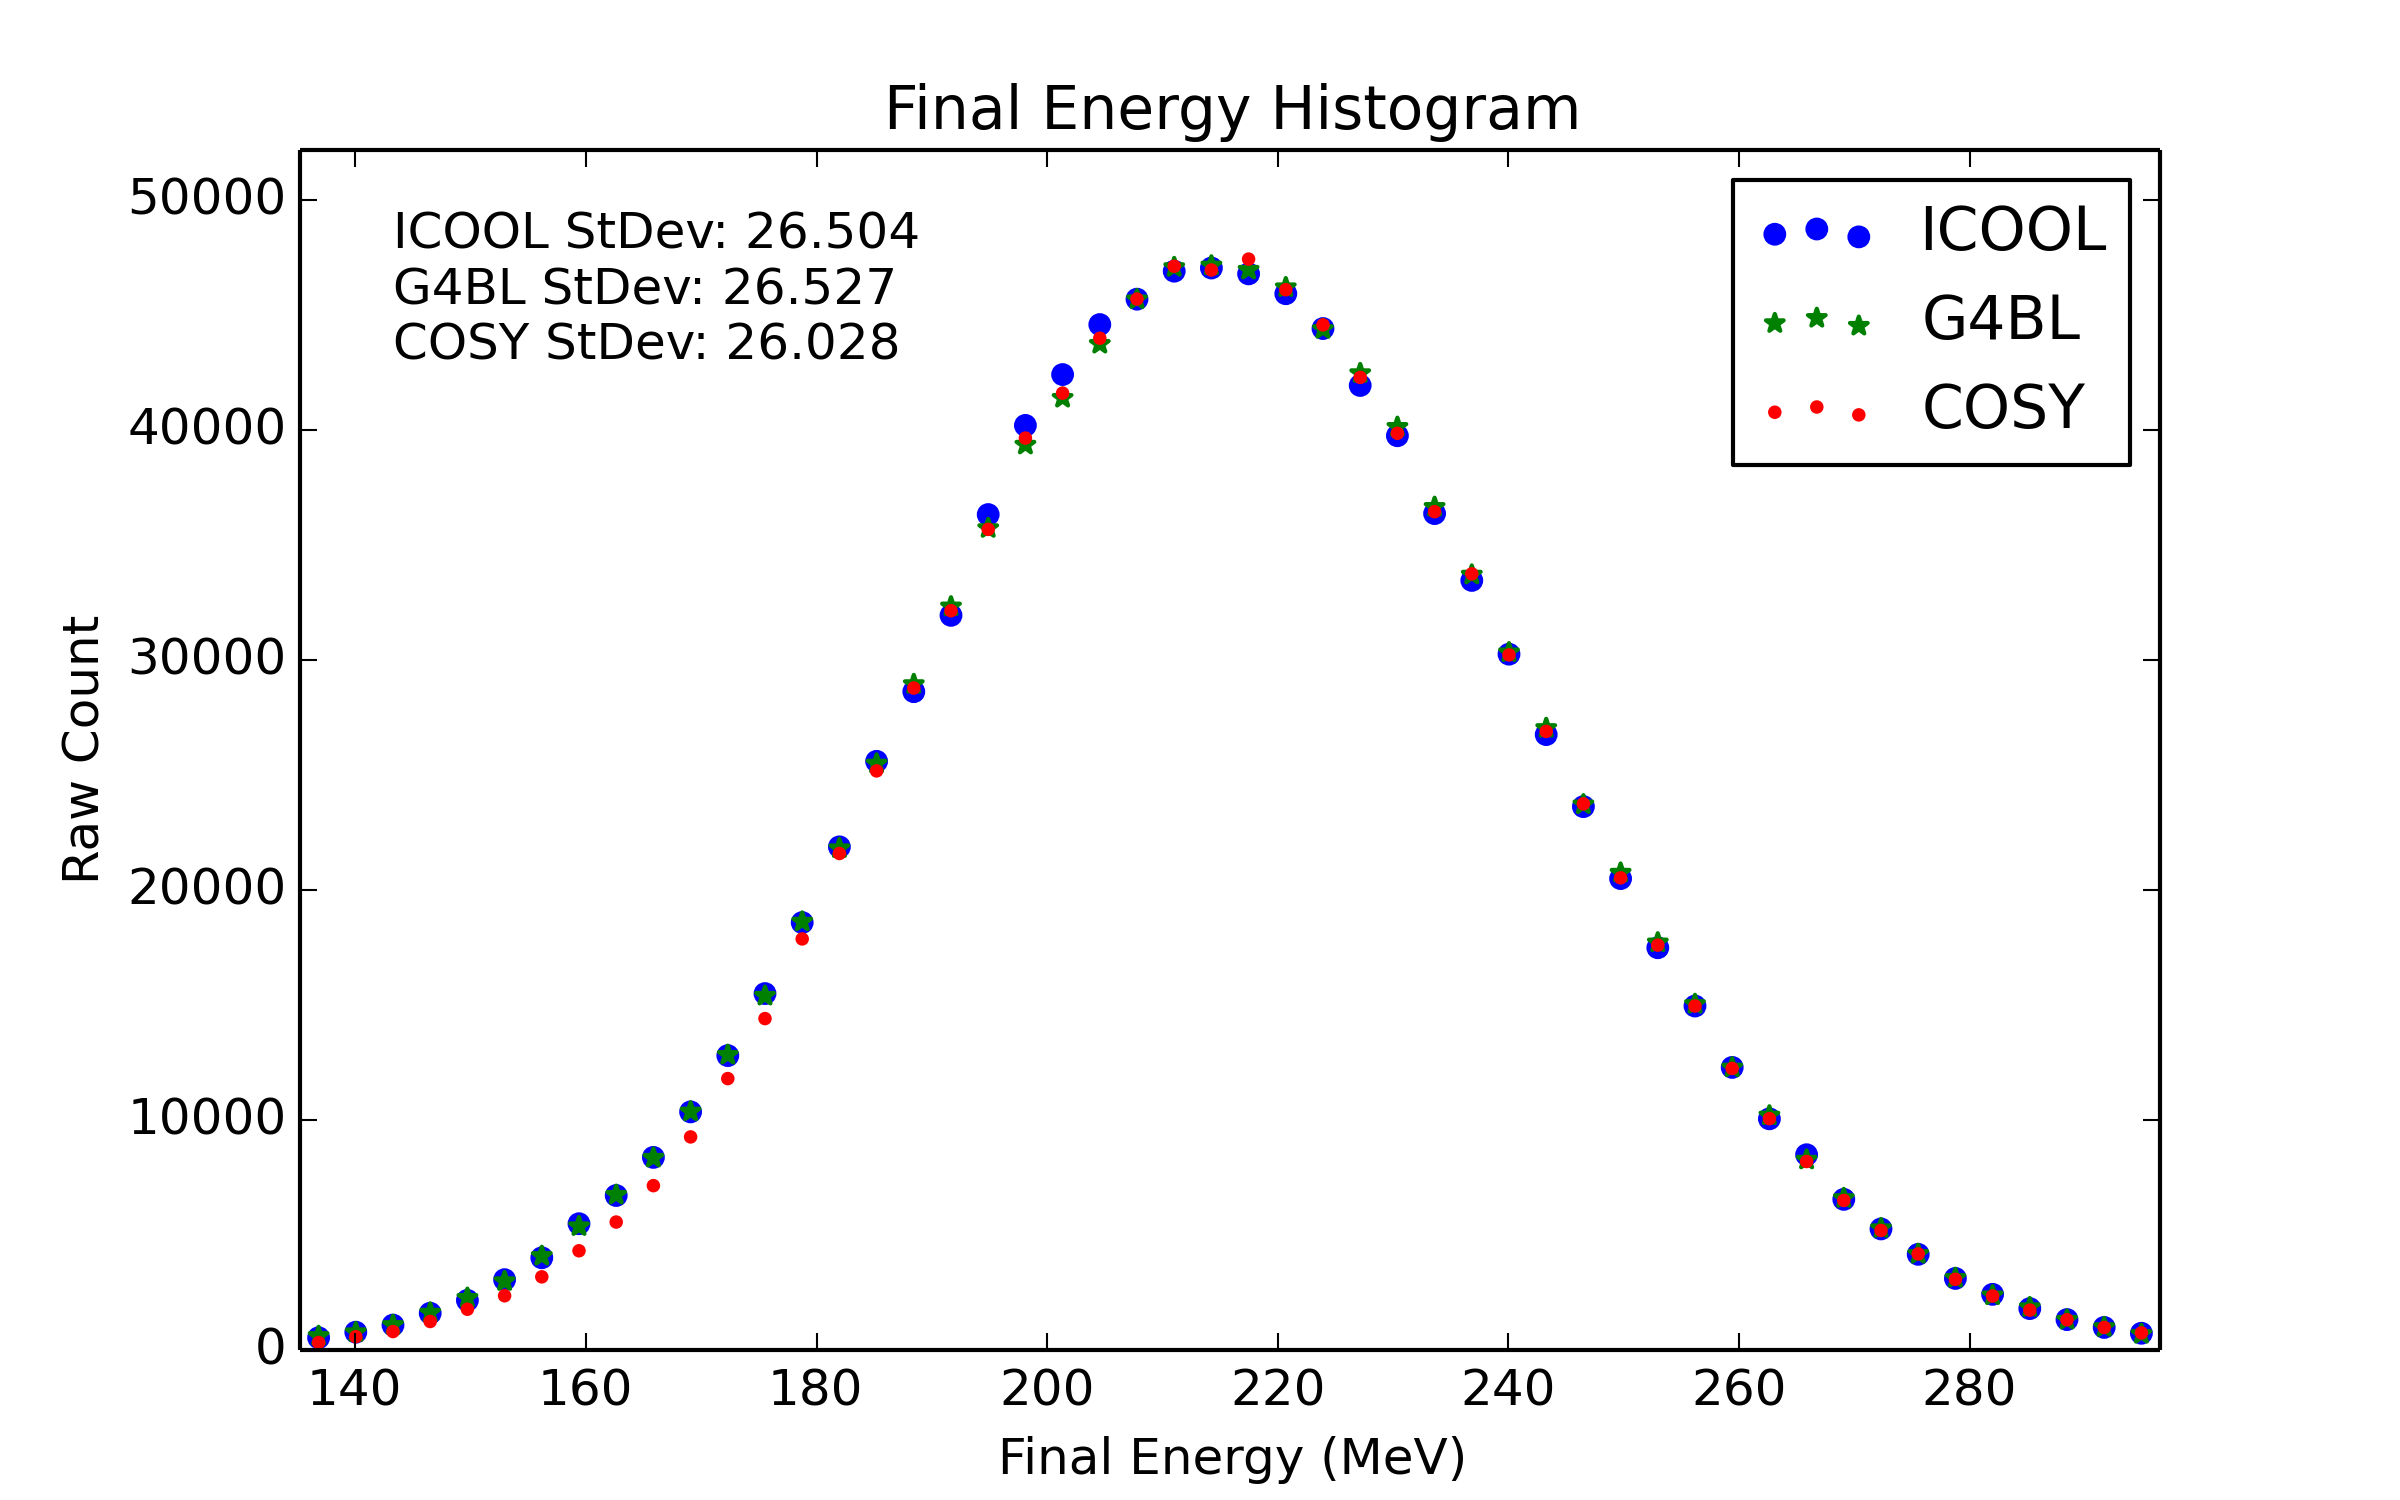
\includegraphics[width=\textwidth]{MICE data/LiH/e} 
  \caption{MICE Step IV final energy results for 65 mm of lithium hydride.}
  \label{fig:mice_lih_energy}
\end{figure}

\Subsection{Step Size Effects}\label{ssc:step_size_effects}
Several step sizes were tested in COSY to ensure optimal efficiency. The results are discussed here.

For the absorber-coil section of MICE liquid hydrogen lattice ($-$0.35/2 to 0.35/2), it was found that 5 steps were sufficient to approximate the superposition of the absorber and coils. To study this step size dependence, $10^5$ particles from the initial distribution found in Table~\ref{tbl:MICE_initial_distribution_parameters} were propagated through the 350 mm liquid hydrogen flat absorber. This simulation took the surrounding magnetic fields into account. Table~\ref{tbl:mice_step_size_ac} shows the effect of changing the step size for the absorber-coil section only.

\begin{table}
\caption*{\textbf{Step Size Dependence for Absorber-Coil Section (Liquid Hydrogen)}}
\begin{center}
\begin{tabularx}{\textwidth}{cccccc}
\hline \hline
& ICOOL & G4BL & \multicolumn{3}{c}{\sout{\hspace{1.5cm}} COSY \sout{\hspace{1.5cm}}}\\
& (field map) & (field map) & 1 step & 5 steps & 10 steps\\
\hline
$\sigma_x$ (mm): & 50.5 & 50.4 & 50.3 & 50.6 & 50.7\\
$\sigma_{\theta_x}$ (mrad): & 201.9 & 201.4 & 205.7 & 200.5 & 199.9\\
$\sigma_E$ (MeV): & 26.7 & 26.7 & 26.6 & 26.6 & 26.6\\
Computational time (s): & 19 & 25 & 4 & 5 & 8\\
\hline
\end{tabularx}
\end{center}
\caption[Step size dependence for the absorber-coil section of MICE Step IV lattice for liquid hydrogen.]{First order step size dependence for the absorber-coil section of MICE Step IV lattice for $10^5$ muons passing through 350 mm of liquid hydrogen. The transmission was very nearly 100\% for all three codes regardless of circumstances. The energy for COSY does not change much with respect to order since the energy loss algorithm does not use a transfer map approach.}
\label{tbl:mice_step_size_ac}
\end{table}

The discrepancy of COSY w.r.t. G4Beamline is $<$1\% for all components. Results of the absorber-coil simulation can be seen in Figures \ref{fig:acx}-\ref{fig:ace}. There is good agreement between ICOOL, G4Beamline, and COSY.

\begin{figure}[H]
  \centering
    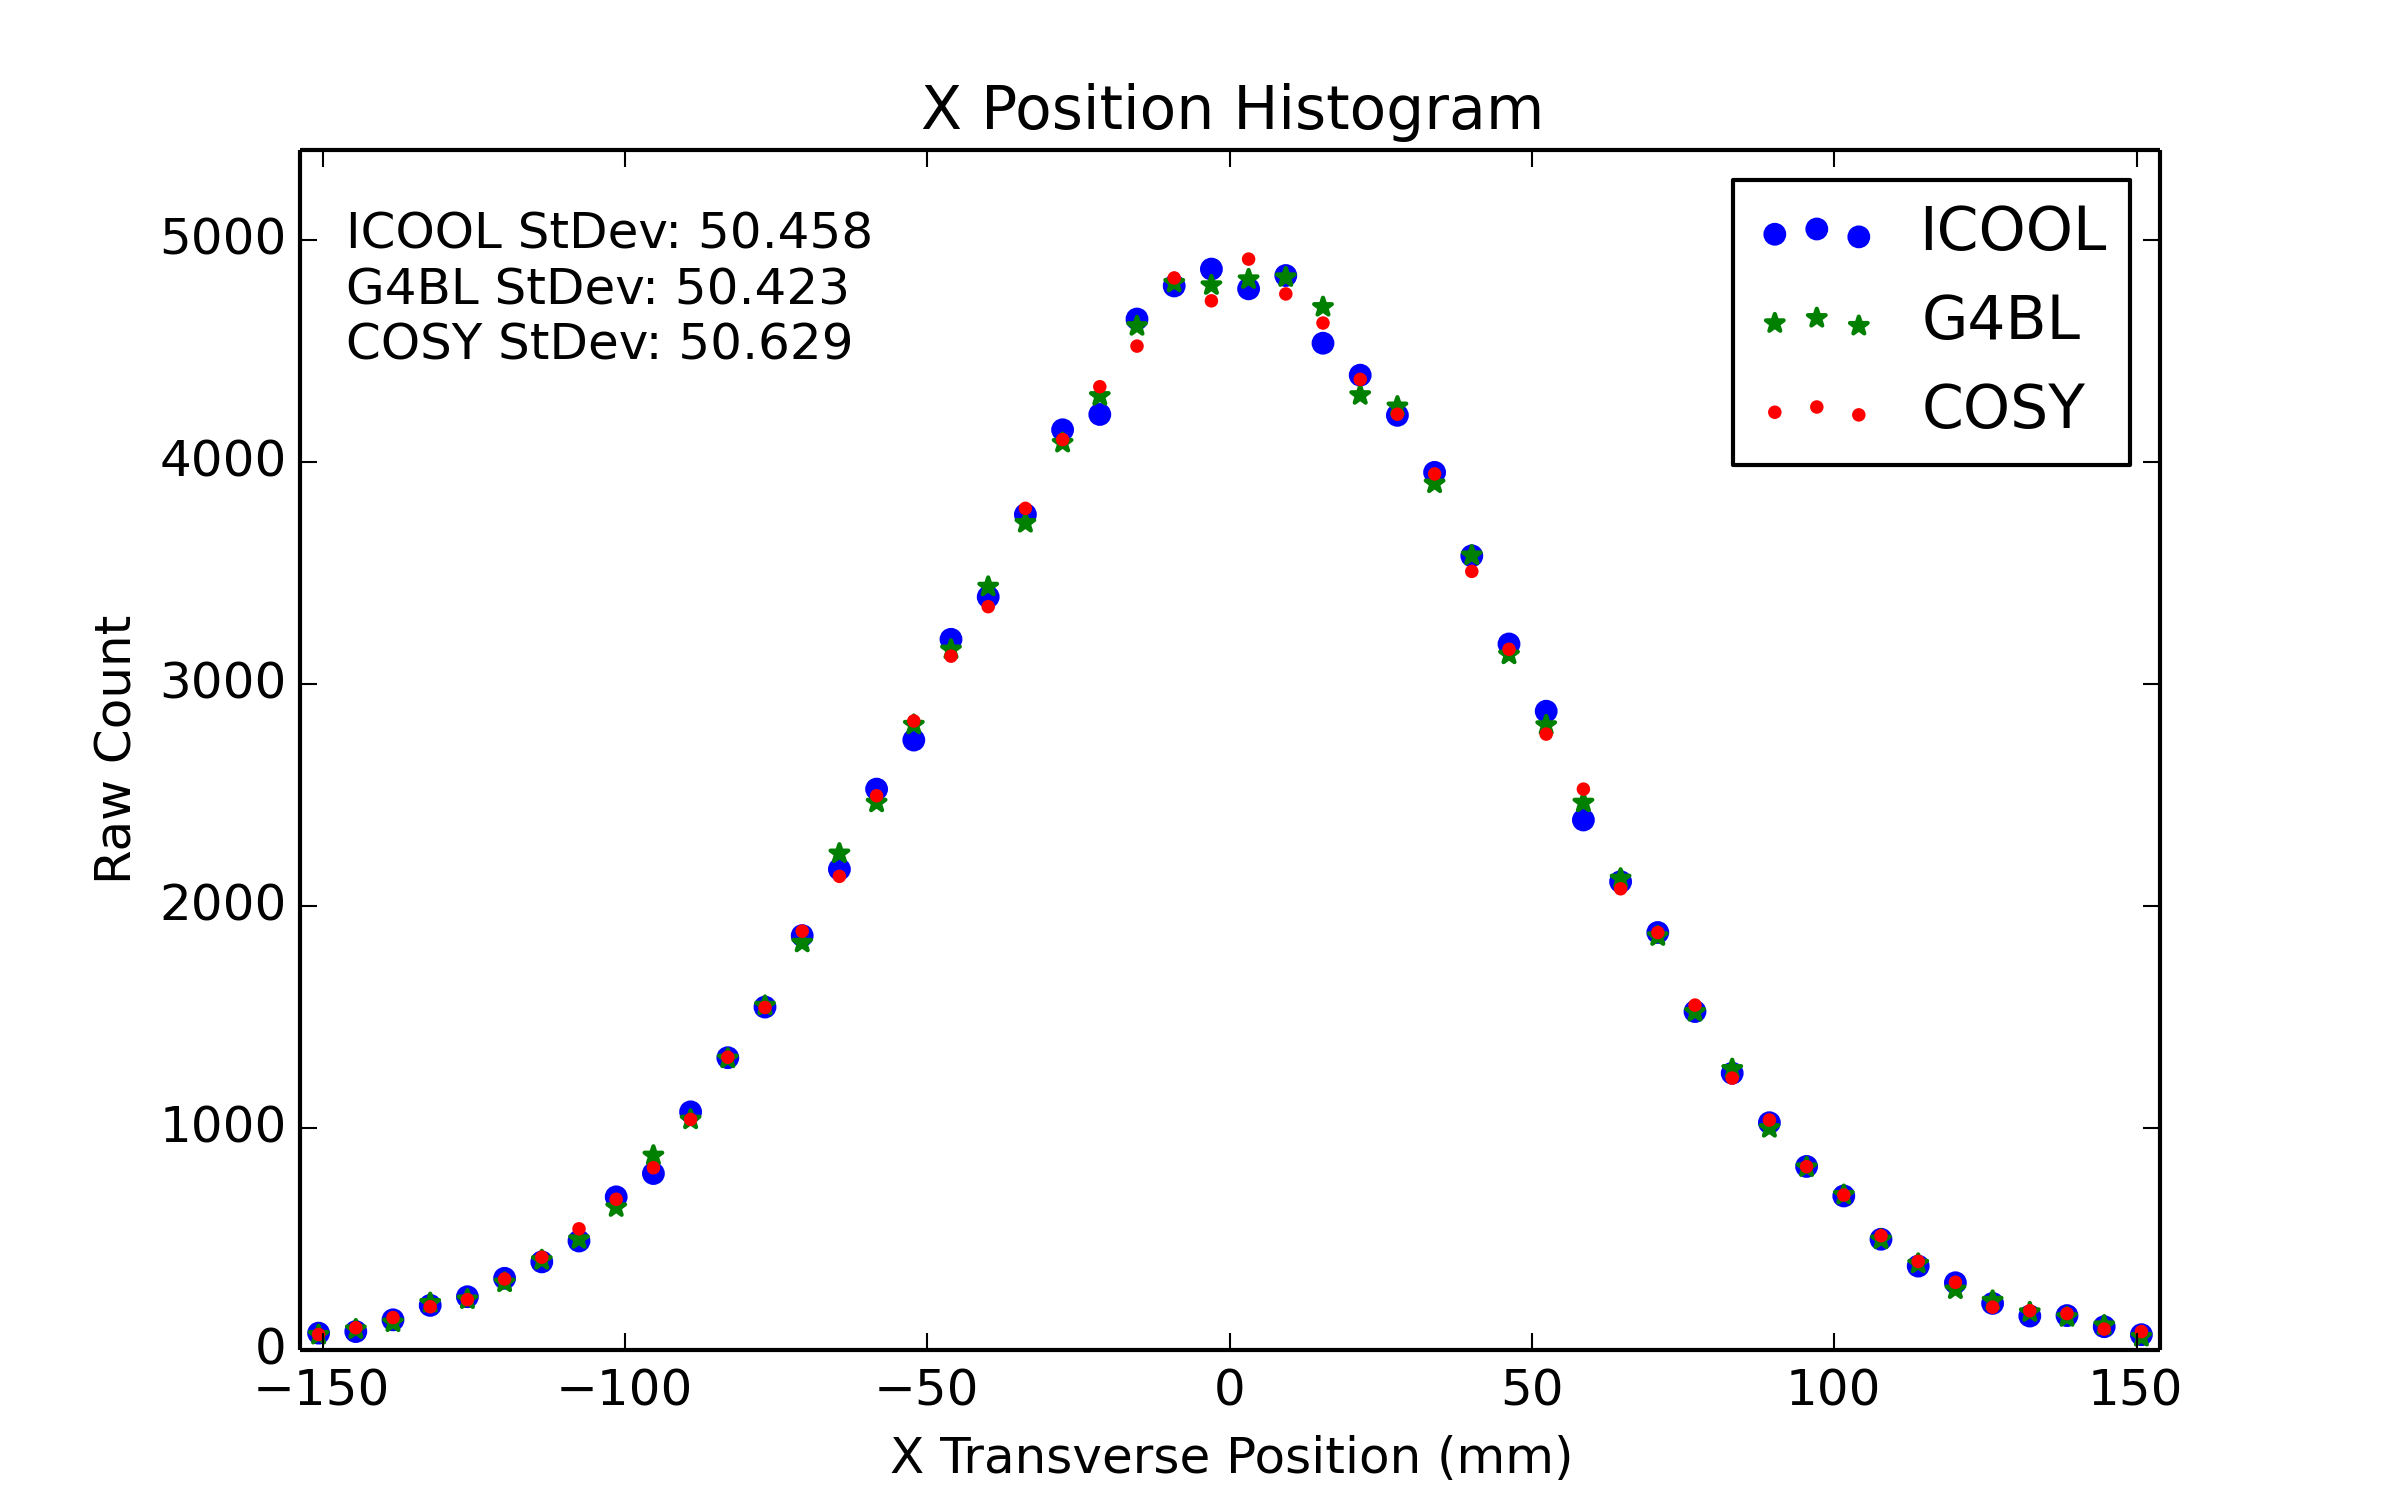
\includegraphics[width=0.7\textwidth]{MICE data/absorber coils/x} 
  \caption{Absorber-coil simulation results for $x$ with $10^5$ muons and a 5 step propagation.}
  \label{fig:acx}
\end{figure}

\begin{figure}[H]
  \centering
    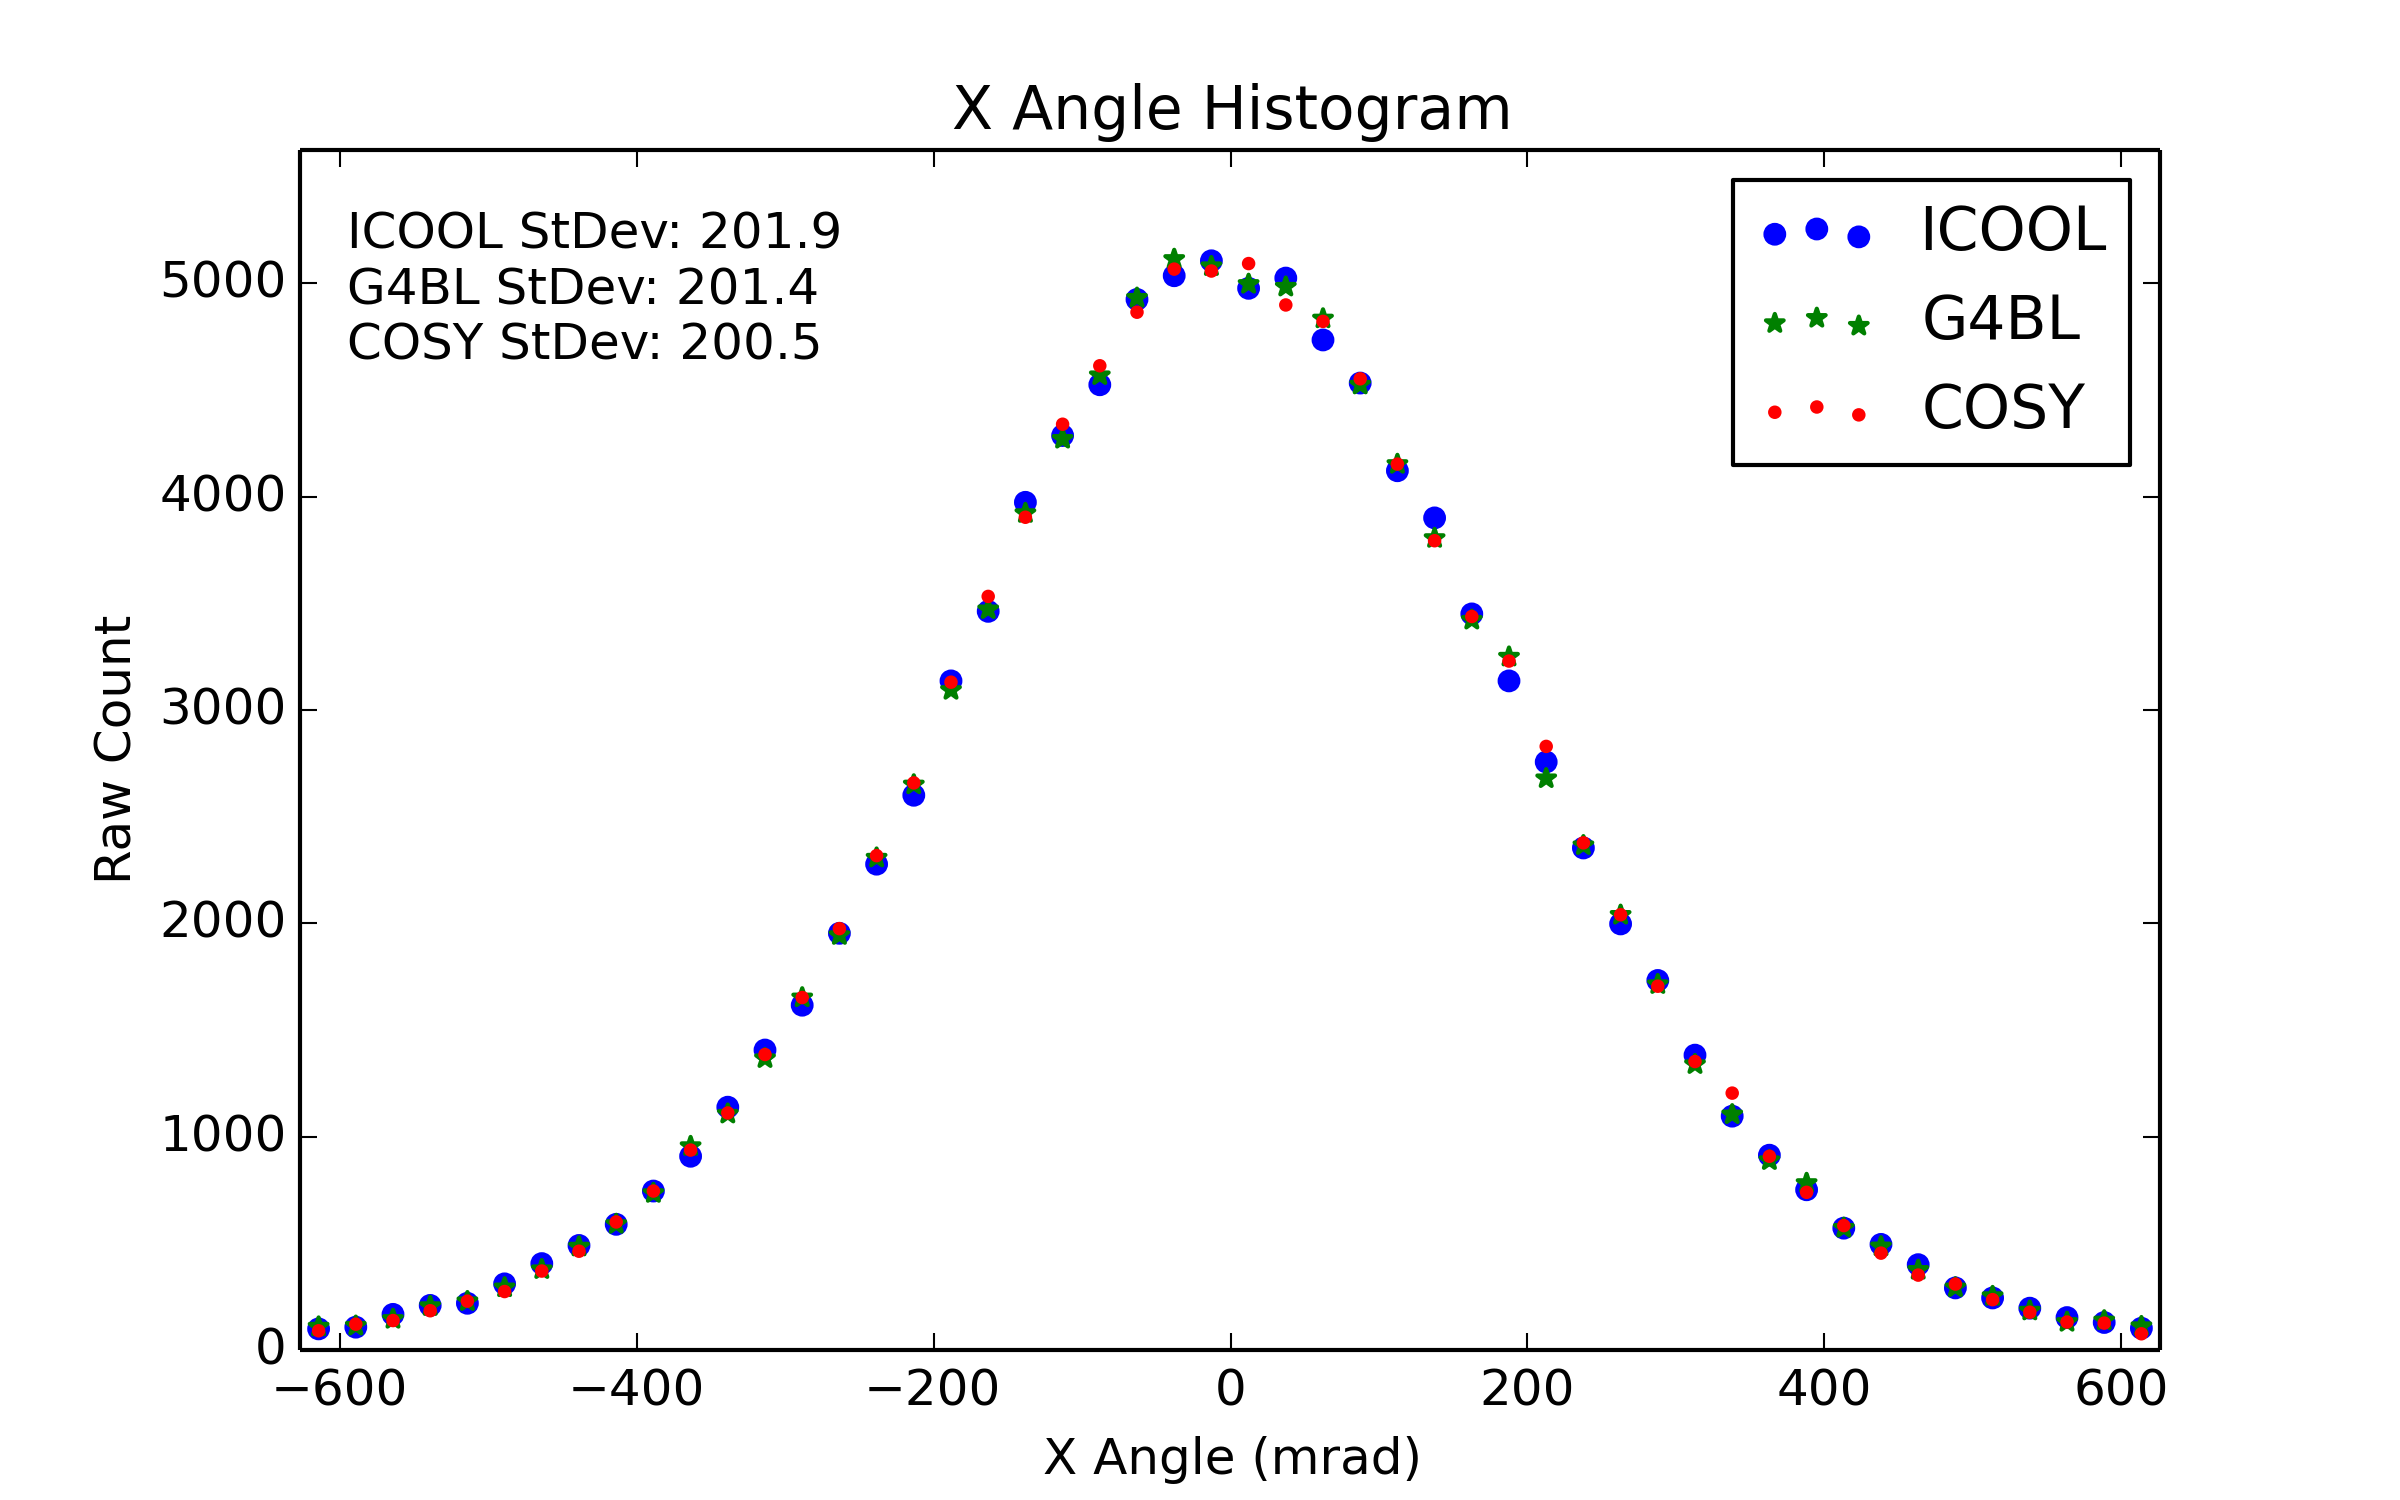
\includegraphics[width=0.7\textwidth]{MICE data/absorber coils/px} 
  \caption{Absorber-coil simulation results for $\theta_x$ with $10^5$ muons and a 5 step propagation.}
  \label{fig:acpx}
\end{figure}

\begin{figure}[H]
  \centering
    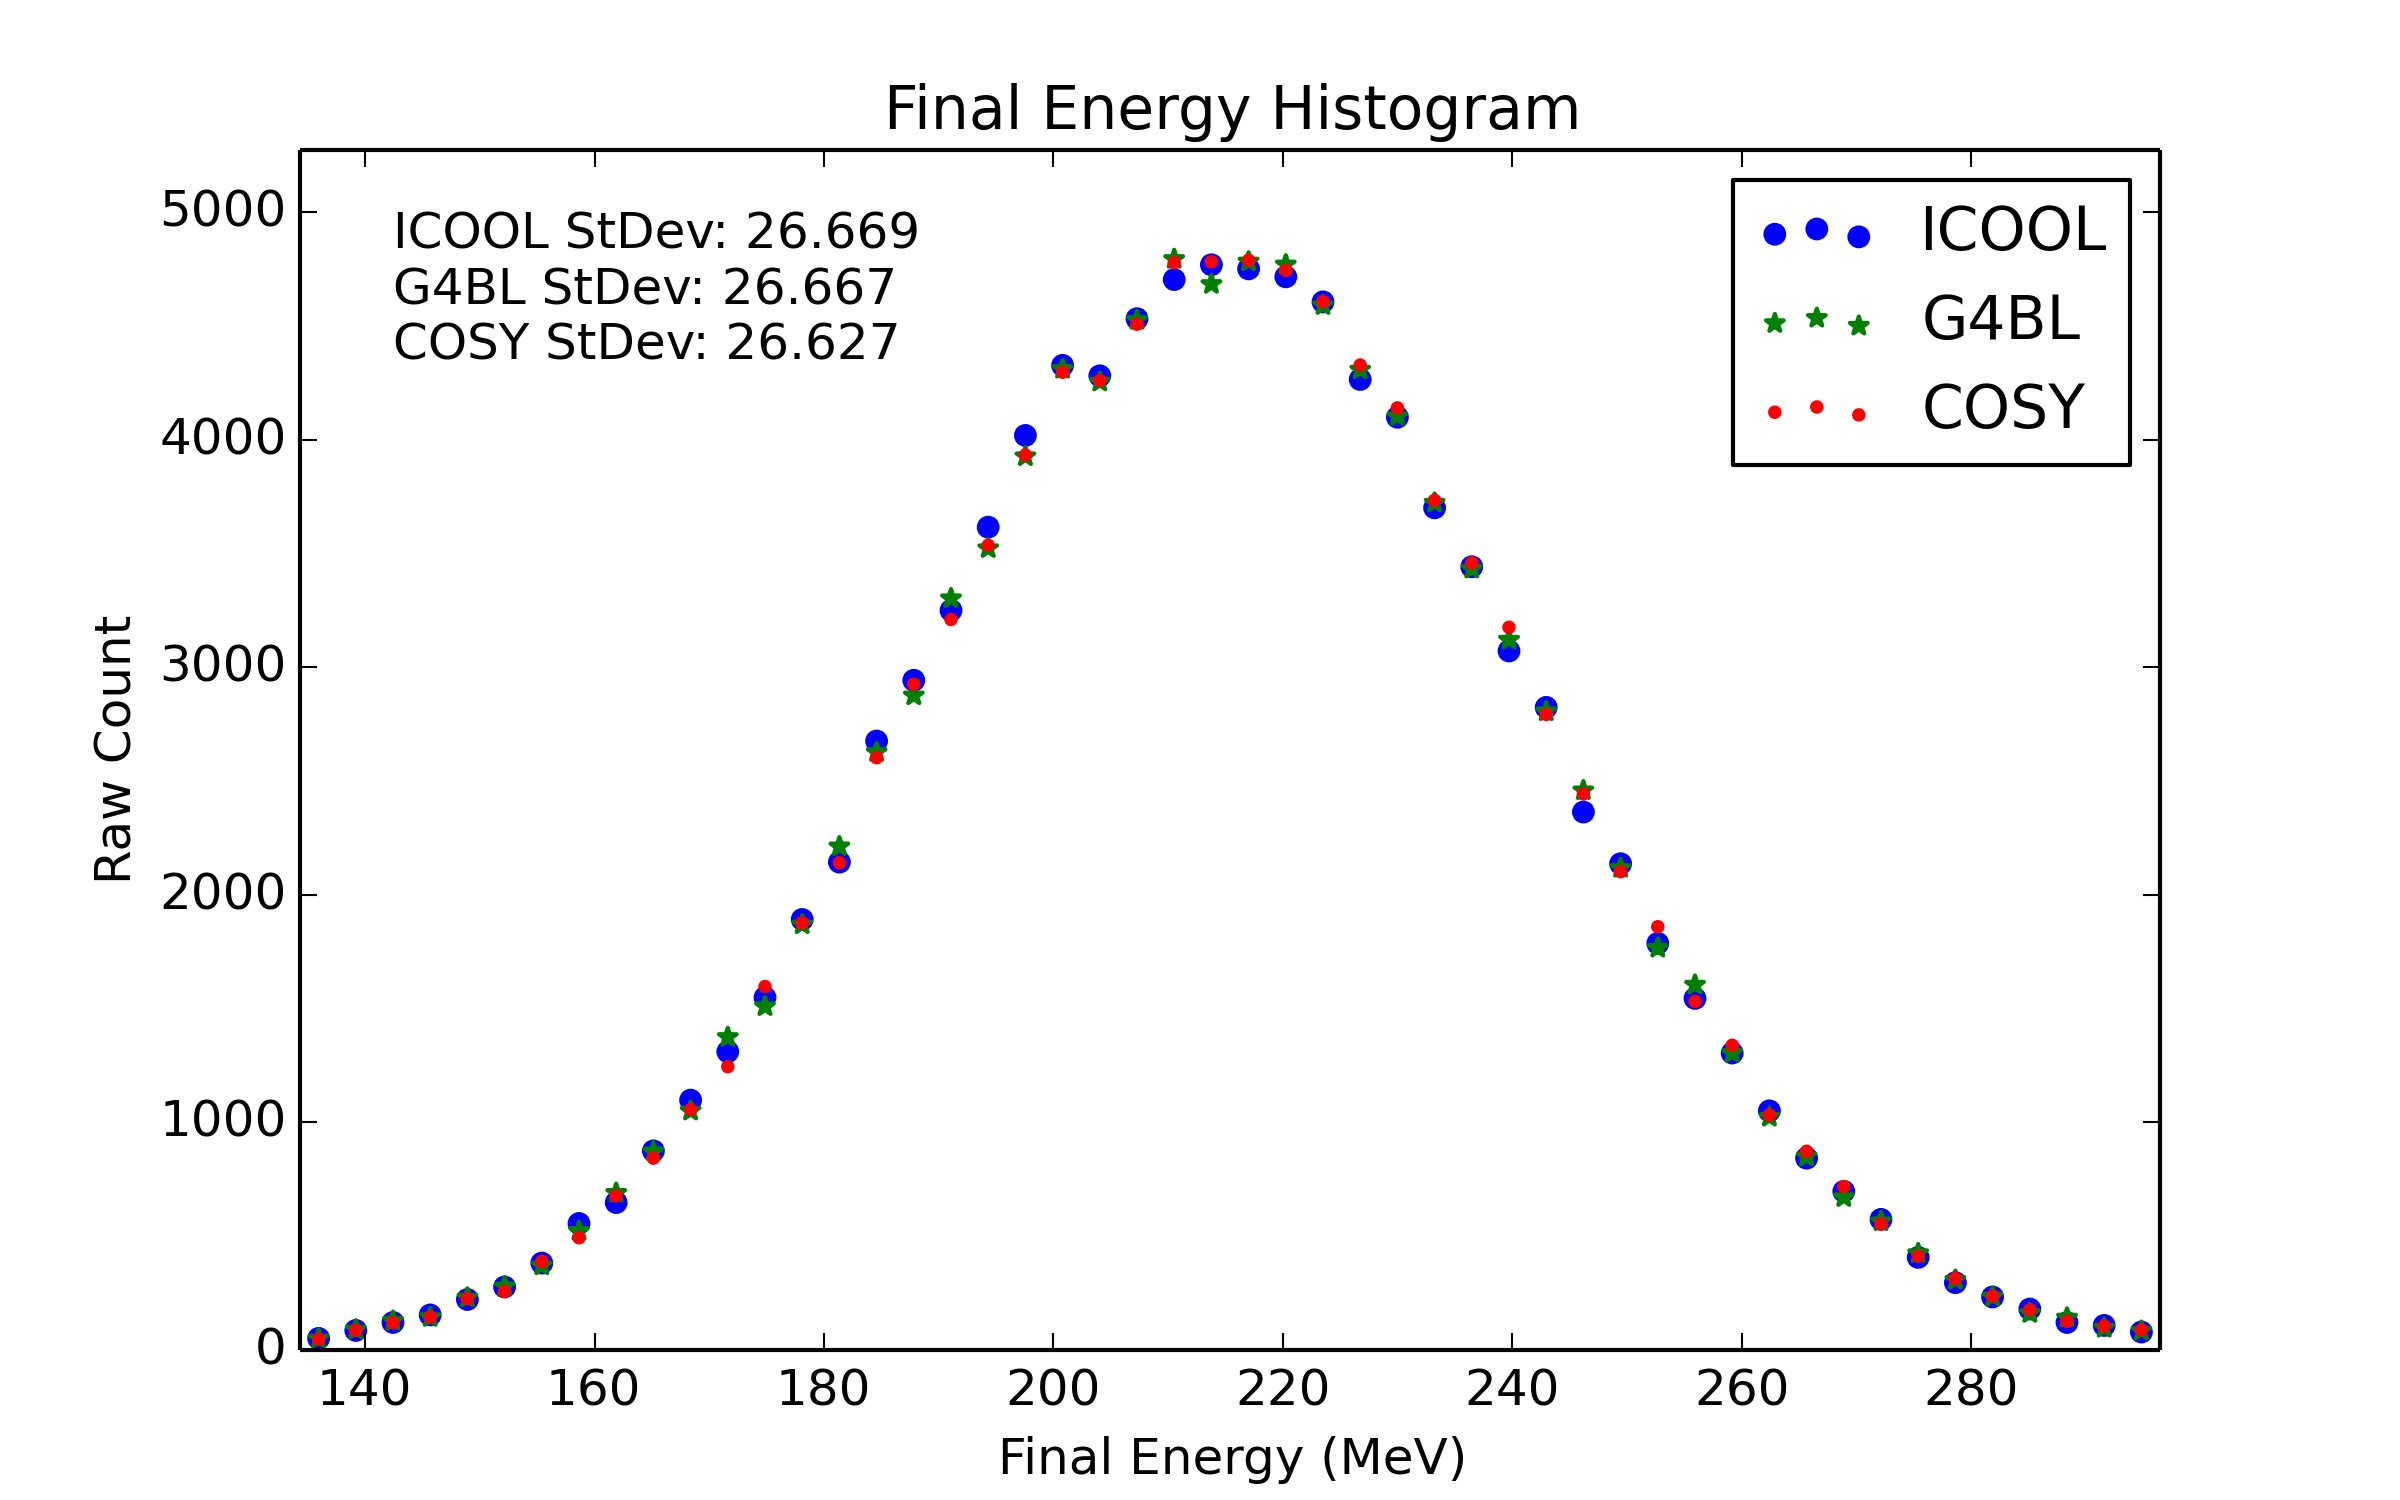
\includegraphics[width=0.7\textwidth]{MICE data/absorber coils/e} 
  \caption{Absorber-coil simulation results for the final energy with $10^5$ muons and a 5 step propagation.}
  \label{fig:ace}
\end{figure}

For both the upstream and downstream sections, the entire MICE cell was simulated ($-2.45105$ m to $2.450$ m). It was found that COSY operated sufficiently well at order 5 and with 50 steps in the simulation.

To study this step size dependence, $10^5$ particles from the initial distribution found in Table~\ref{tbl:MICE_initial_distribution_parameters} were propagated through MICE cell. Table~\ref{tbl:mice_step_size_upstream} shows the effect of changing the step size.

\begin{table}
\caption*{\textbf{Step Size Dependence for MICE Step IV}}
\begin{center}
\begin{tabularx}{\textwidth}{cccccccc}
\hline \hline
& ICOOL & G4BL & \multicolumn{5}{c}{COSY [order]@[number of steps]}\vspace{-12pt}\\
& (field map) & (field map) & 3@50 & 5@30 & 5@50 & 5@100 & 7@100\\
\hline
$\sigma_x$ (mm): & 40.7 & 40.7 & 42.5 & 41.2 & 41.4 & 41.4 & 41.0\\
$\sigma_{\theta_x}$ (mrad): & 240.2 & 240.2 & 248.3 & 239.8 & 242.1 & 243.8 & 241.8\\
\% transmission: & 98.5 & 98.5 & 99.6 & 96.8 & 97.7 & 98.6 & 97.9\\
Comp. time (s): & 114 & 82 & 12 & 21 & 25 & 43 & 132\\
\hline
\end{tabularx}
\end{center}
\caption[Step size dependence for MICE Step IV lattice.]{Step size dependence for MICE Step IV lattice for $10^5$ muons. The notation for COSY is [order]@[number of steps].}
\label{tbl:mice_step_size_upstream}
\end{table}

For most COSY cases, the discrepancy w.r.t. G4Beamline is on the order of 1\%. 5th order at 50 steps was selected as ``best'' because of the increased agreement with both ICOOL and G4Beamline when compared to both 3@50 and 5@30 (particularly for the transmission). Moreover, 5@50 gives similar results as 7@100 but with drastically decreased computational time. 

Results of the step size study for 5@50 can be seen in Figures \ref{fig:upx} and \ref{fig:uppx}. There is good agreement between ICOOL, G4Beamline, and COSY.

\begin{figure}[H]
  \centering
    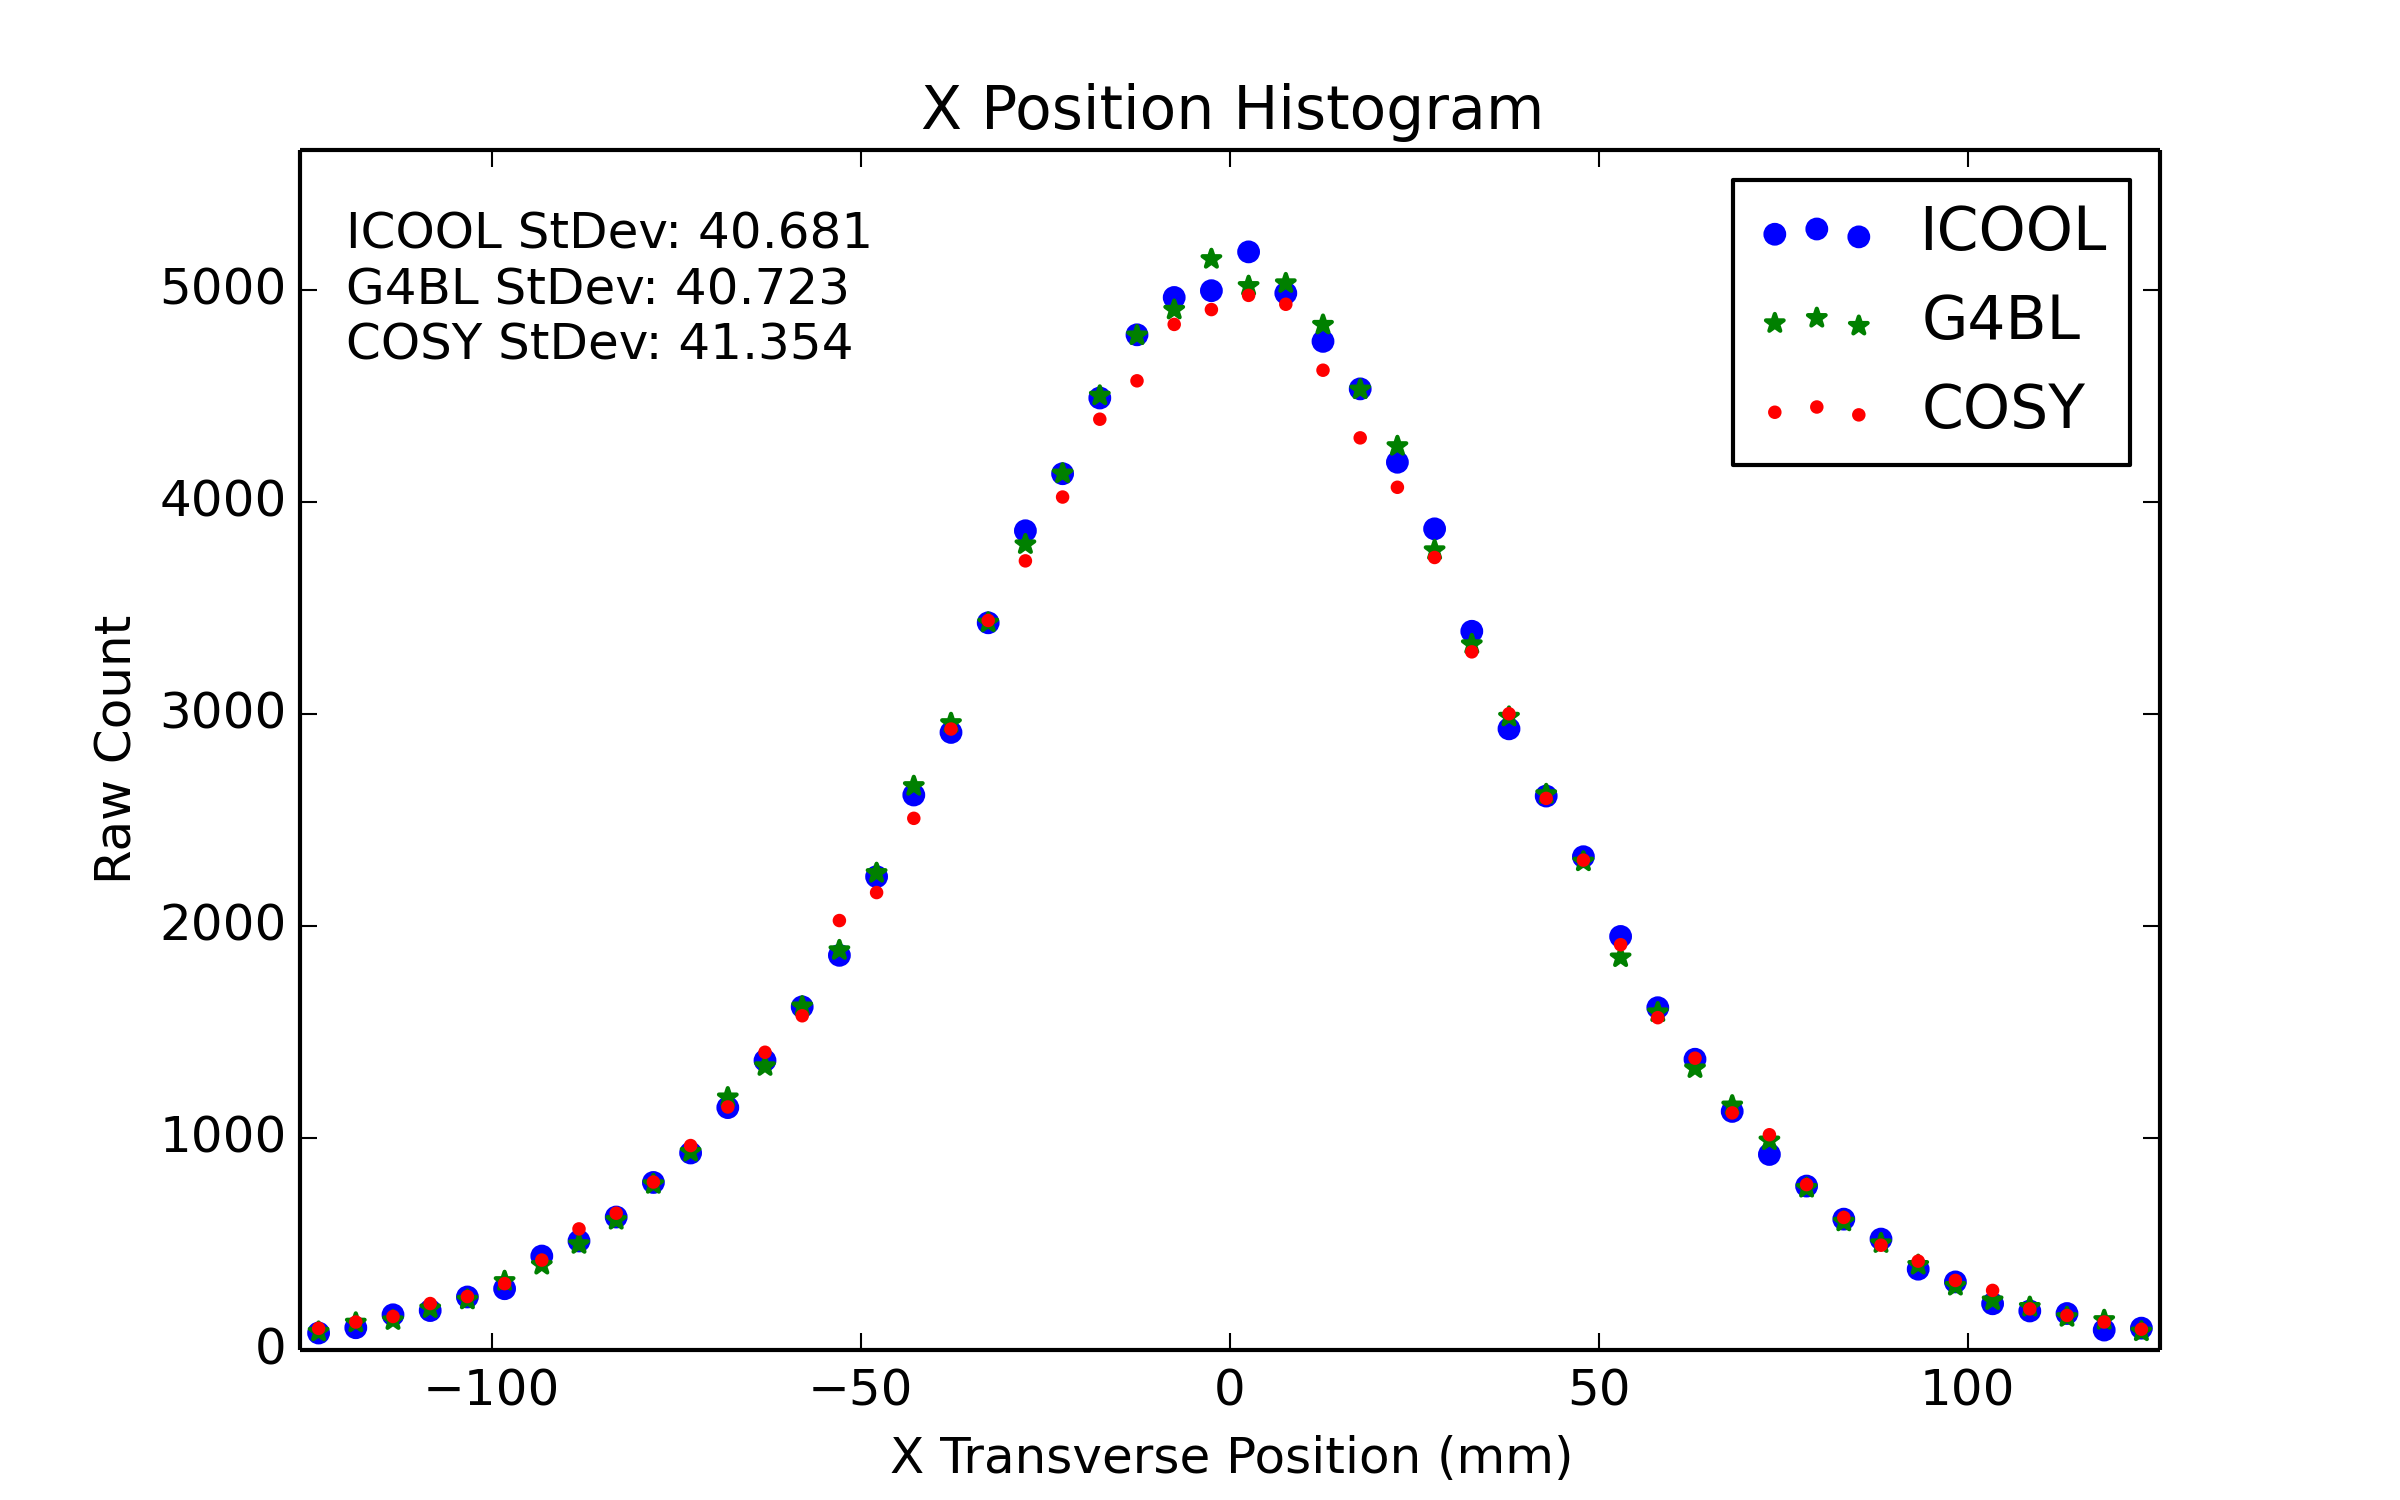
\includegraphics[width=0.7\textwidth]{MICE data/upstream/x} 
  \caption{MICE simulation results for $x$ with $10^5$ muons at 5th order and 50 steps.}
  \label{fig:upx}
\end{figure}

\begin{figure}[H]
  \centering
    \includegraphics[width=0.7\textwidth]{MICE data/upstream/px} 
  \caption{MICE simulation results for $\theta_x$ with $10^5$ muons at 5th order and 50 steps.}
  \label{fig:uppx}
\end{figure}

\Section{Summary}\label{sec:summary}

In summary, new simulation tools for muon ionization cooling have been added to COSY Infinity for particle-by-particle propagation. The energy straggling, multiple scattering, transverse position, and time-of-flight models were developed from first principles. The algorithms implemented have been modified via empirical fit to MuScat \cite{muscat} while keeping reasonable agreement with G4Beamline. Fitted with this new software, COSY has simulated one of the current muon ionization cooling efforts, MICE Step IV \cite{mice}, yielding agreement within 1\% of both ICOOL and G4Beamline. The code developed in this work is accurate, fast, and user-friendly.